\documentclass[a4paper]{article}


\linespread{1.3}

\usepackage[top=1.8cm,bottom=1.8cm,left=3cm,right=3cm,marginparwidth=1.75cm]{geometry}
\usepackage{listings}
\usepackage{courier}
\usepackage{graphicx}
\usepackage{float}
\usepackage{xcolor}
\usepackage[utf8]{inputenc}
\usepackage[T1]{fontenc}
\usepackage[polish]{babel}
\usepackage[linesnumbered,ruled,vlined]{algorithm2e}
\usepackage{url}
\usepackage{xurl}
\usepackage{amsmath}
\usepackage{microtype}
\usepackage[hidelinks]{hyperref}
\usepackage{booktabs}
\usepackage{array}

\SetAlgorithmName{Algorytm}{Algorytm}{Spis algorytmów}


\sloppy

\title{UMA - las, turniej\\
Dokumentacja końcowa}
\author{Michał Suski 331439, Kamil Marszałek 331401}
\date{}

\begin{document}

\maketitle

\section{Treść zadania}
Zmodyfikowany las losowy w zadaniu klasyfikacji. Podczas budowy każdego z drzew testy (z pełnego zbioru testów) wybieramy za pomocą turnieju: \url{https://staff.elka.pw.edu.pl/~rbiedrzy/UMA/turniejRuletka.pdf}, czyli wybieramy losowo 2 testy, liczymy ich jakość, stosujemy ten z wyższą jakością. Do wstępnych testów polecam zbiór danych z zadaniem klasyfikacji grzybów: \url{https://archive.ics.uci.edu/dataset/73/mushroom}, na którym powinno dać się uzyskać wyniki w okolicy 100\%. Do dalszych testów należy znaleźć i pobrać inne zbiory danych (na wskazanej stronie lub w Kaggle). Przed rozpoczęciem realizacji projektu proszę zapoznać się z zawartością: \url{https://staff.elka.pw.edu.pl/~rbiedrzy/UMA/index.html}.

\section{Interpretacja i opis algorytmu}

Projekt ma na celu sprawdzenie, czy wybór testów (podziałów węzłów) za pomocą prostego turnieju dwuelementowego poprawi własności klasycznego lasu losowego, w szczególności:
\begin{itemize}
    \item zmniejszy skłonność pojedynczych drzew do przeuczenia,
    \item zwiększy \emph{różnorodność} drzew w lesie (mniejsza korelacja pomiędzy drzewami),
    \item nie pogorszy istotnie jakości klasyfikacji w porównaniu z klasycznym wyborem najlepszego testu.
\end{itemize}



Funkcja wyboru testu (zachłannie lub turniejowo) oraz sposób oceny jego jakości będą parametrami modelu budującego las. Ułatwi to porównanie ich wpływu na skuteczność algorytmu.

\begin{itemize}
    \item Zaimplementowane zostaną dwa typy drzew: podstawowe \textbf{ID3} oraz \textbf{CART}, dla lepszej obsługi atrybutów ciągłych.
    \item Dla drzew \textbf{CART} zostanie zaimplementowana osobna funkcja oceny jakości podziału (indeks Giniego) oraz sposób kodowania atrybutów kategorycznych \textbf{one-hot encoding}.
\end{itemize}




\subsection{Miary jakości testu}

Test (podział) węzła $S$ dzieli zgromadzone w nim przykłady na dwa (dla CART) lub więcej (dla ID3) podzbiorów. Jakość testu określamy na podstawie \emph{nieczystości} węzła przed i po podziale.
Dla węzła z podzbiorem $S$ definiujemy udział klasy $k$:
\[
p_k(S) = \frac{1}{|S|} \bigl|\{(x_i, y_i) \in S : y_i = k\}\bigr|
\]
Przykładowe miary nieczystości:
\begin{itemize}
    \item \textbf{Entropia:}
    \[
        H(S) = - \sum_{k=1}^K p_k(S)\,\log_2 p_k(S)
    \]
    \item \textbf{Indeks Giniego:}
    \[
        G(S) = 1 - \sum_{k=1}^K p_k(S)^2
    \]
\end{itemize}
Niech test $t$ dzieli bazowy węzeł $S$ na podzbiory $S_1, \dots, S_m$. Wtedy:
\begin{itemize}
    \item \textbf{Information Gain}:
    \[
        IG(t, S) = H(S) - \sum_{j=1}^{m} \frac{|S_j|}{|S|} H(S_j)
    \]
    \item \textbf{Gini Gain}:
    \[
        GG(t, S) = G(S) - \sum_{j=1}^{m} \frac{|S_j|}{|S|} G(S_j)
    \]
\end{itemize}
W dalszej części projektu planujemy użyć:
\begin{itemize}
    \item dla drzew ID3: domyślnie \textbf{Information Gain} oraz opcjonalnie \textbf{Gain Ratio} lub \textbf{Gini Gain},
    \item dla drzew CART: \textbf{Gini Gain}.
\end{itemize}




\section{Zbiory danych}

\begin{enumerate}
    \item \textbf{Klasyfikacja grzybów} \\
    Źródło: \url{https://archive.ics.uci.edu/dataset/73/mushroom}

    \begin{description}
        \item[Typ zadania:] klasyfikacja binarna (grzyb jadalny / trujący)
        \item[Liczba przykładów:] 8124
        \item[Jadalne:] 4208
        \item[Trujące:] 3916
        \item[Liczba atrybutów:] 22
        \item[Typ atrybutów:] wszystkie dyskretne
        \item[Uwagi:] zbiór prosty, klasy zbalansowane, przewidywana dokładność bliska 100\%
    \end{description}

    \item \textbf{Zaległości płatnicze klientów kart kredytowych} \\
    Źródło: \url{https://archive.ics.uci.edu/dataset/350/default+of+credit+card+clients}

    \begin{description}
        \item[Typ zadania:] klasyfikacja binarna (czy klient będzie zalegał z płatnością w przyszłym miesiącu?)
        \item[Liczba przykładów:] 30000
        \item[Brak zaległości:] 23364
        \item[Zaległość:] 6636
        \item[Liczba atrybutów:] 23
        \item[Typ atrybutów:] ciągłe i dyskretne (liczbowe)
        \item[Uwagi:] Klasy są niezbalansowane. Występuje duża liczba atrybutów ciągłych, co czyni go idealnym do testowania wydajności progów w algorytmie CART. Nie spodziewamy się dokładności 100\%.
    \end{description}

     \item \textbf{Skuteczność marketingu banku} \\
    Źródło: \url{https://archive.ics.uci.edu/dataset/222/bank+marketing}

    \begin{description}
        \item[Typ zadania:] klasyfikacja binarna (czy klient założy lokatę?)
        \item[Liczba przykładów:] 45211
        \item[Nie założy lokaty:] 39922
        \item[Założy lokatę:] 5289
        \item[Liczba atrybutów:] 16
        \item[Typ atrybutów:] dyskretne i ciągłe
        \item[Uwagi:] Klasy są niezbalansowane -- trzeba zadbać, aby nie wpłynęło to na algorytm. Atrybuty ciągłe obsłużone progiem (CART). Zbiór powinien dobrze pokazywać różnice przy testowaniu różnych funkcji oceny jakości testu. Nie spodziewamy się dokładności 100\%.
    \end{description}

    \item \textbf{Nawrót raka piersi (Breast Cancer)} \\
    Źródło: \url{https://archive.ics.uci.edu/dataset/14/breast+cancer}

    \begin{description}
        \item[Typ zadania:] klasyfikacja binarna (czy nastąpi nawrót choroby?)
        \item[Liczba przykładów:] 286
        \item[Brak nawrotu:] 201
        \item[Nawrót:] 85
        \item[Liczba atrybutów:] 9
        \item[Typ atrybutów:] dyskretne
        \item[Uwagi:] Zbiór posiada niewiele przykładów, co pozwoli sprawdzić tendencje do przeuczania. Występują nieliczne braki danych, które wymagają obsłużenia przed procesem uczenia. Przykłady nie są trywialne, przez co spodziewamy się dokładności poniżej 100\%.
    \end{description}
\end{enumerate}



    Aby zastosować zbiory \textbf{2} oraz \textbf{3} do drzew ID3 konieczne byłoby zdyskretyzowanie atrybutów ciągłych. Wprowadzałoby to jednak problemy z reprezentatywnością danych (na przykład mogłoby wprowadzić dodatkowe, pierwotnie nieistniejące zależności), dlatego zbiory te zostaną \textbf{pominięte} w procesie badania algorytmu ID3.



\subsection{Metody podziału danych na zbiory trenujący i testowy}

Bazową proporcją dla zbiorów trenującego / testowego będzie 70\% / 30\% -- ten podział będzie \textbf{stratyfikowany} względem klas, aby zachować ich oryginalne proporcje. Do budowy pojedynczego drzewa wylosowana zostanie próbka danych ze zbioru trenującego.

\section{Wybór technologii}

Projekt został zaimplementowany w języku \textbf{Python} z wykorzystaniem bibliotek \textbf{NumPy} oraz \textbf{pandas}, które posłużą odpowiednio do obliczeń numerycznych i przetwarzania danych. W celu oceny jakości proponowanego rozwiązania oraz porównania jego skuteczności, jako punkt odniesienia zostanie wykorzystany klasyczny las losowy z pakietu \textbf{scikit-learn}.

\section{Metodyka eksperymentalna}

Przebieg pojedynczego uruchomienia badania:
\begin{itemize}
    \item Podział zbioru danych na trenujący (70\%) i testowy (30\%) w sposób stratyfikowany.
    \item Budowa lasu na zbiorze trenującym zgodnie z ustalonymi parametrami.
    \item Użycie lasu do predykcji na zbiorze testowym oraz zebranie wyników.
\end{itemize}

Z uwagi na użycie w badanych modelach generatorów liczb pseudolosowych, przedstawiane w tym dokumencie wyniki będą zagregowane z \textbf{25 niezależnych uruchomień} takiego samego eksperymentu.
\begin{itemize}
    \item Aby wyniki badań były powtarzalne, w skład parametrów eksperymentu wchodzi ziarno generatora liczb pseudolosowych.
    \item Przy każdej iteracji badania według tego ziarna dokonywany jest podział zbioru danych na zbiory trenujący i testowy oraz w sposób deterministyczny generowane są ziarna cząstkowe służące do budowy pojedynczych drzew.
\end{itemize}

W celu usprawnienia wykonywania badań zdefiniowany został system, który pobiera parametry eksperymentu z plików \textit{.csv}, wykonuje zlecone badania i zapisuje wyniki do późniejszej analizy.
Jako parametr podawane jest bazowe ziarno, które następnie w każdej iteracji jest inkrementowane, co zapewnia powtarzalność pomiarów.


Drzewa ID3 zostaną przetestowane na zbiorach \textbf{1} i \textbf{4}, natomiast drzewa CART na \textbf{wszystkich czterech} zbiorach. Drzewo z biblioteki \textit{scikit-learn} jest typu CART, dlatego w porównaniu zostanie uwzględnione również na \textbf{wszystkich czterech} zbiorach.


\section{Miary jakości eksperymentów}
\label{sec:miary-jakosci}

Dla każdego eksperymentu będziemy raportować:


\subsection{Miary podstawowe}

\begin{itemize}
    \item Średnia arytmetyczna (uzyskanej dokładności)
    \item Najlepszy wynik
    \item Najgorszy wynik
    \item Średni czas budowy lasu
    \item Odchylenie standardowe:

        Dla serii $n$ powtórzeń tego samego eksperymentu, odchylenie standardowe z próby definiujemy jako:

    \[
    s = \sqrt{\frac{1}{n-1} \sum_{i=1}^{n} (x_i - \bar{x})^2}
    \]

    \noindent gdzie:
    \begin{itemize}
        \item $n$ -- liczba powtórzeń eksperymentu,
        \item $x_i$ -- wynik (dokładność) uzyskany w $i$-tym powtórzeniu,
        \item $\bar{x}$ -- średnia arytmetyczna wyników ze wszystkich powtórzeń: $\bar{x} = \frac{1}{n} \sum_{i=1}^{n} x_i$.
    \end{itemize}
\end{itemize}

Te miary przedstawią ogólny obraz wyników modelu.

\subsection{Macierz pomyłek i dokładność}

Dla binarnej klasyfikacji definiujemy macierz pomyłek:

\begin{center}
\begin{tabular}{c|cc}
 & Predykcja: pozytywna & Predykcja: negatywna \\
\hline
Rzeczywista: pozytywna & TP & FN \\
Rzeczywista: negatywna & FP & TN \\
\end{tabular}
\end{center}

\noindent gdzie:
\begin{itemize}
    \item TP -- (ang. true positives) poprawnie rozpoznane przykłady pozytywne,
    \item TN -- (true negatives) poprawnie rozpoznane przykłady negatywne,
    \item FP -- (false positives) negatywne zaklasyfikowane jako pozytywne,
    \item FN -- (false negatives) pozytywne zaklasyfikowane jako negatywne.
\end{itemize}
\textbf{Dokładność (accuracy)} zdefiniowana jest jako:
\[
\text{Dokładność} = \frac{TP + TN}{TP + TN + FP + FN}
\]

\subsection{Precyzja, czułość i F1-score}

Dla klasy pozytywnej definiujemy:
\[
\text{Precyzja} = \frac{TP}{TP + FP}, \quad
\text{Czułość} = \frac{TP}{TP + FN}
\]

\[
F1 = \frac{2 \cdot \text{Precyzja} \cdot \text{Czułość}}{\text{Precyzja} + \text{Czułość}}
\]

Miary te są szczególnie istotne przy niezbalansowanych zbiorach (np. Adult, Bank Marketing), gdzie sama dokładność może być myląca.

\section{Wpływ hiperparametrów na jakość modelu}

Jako domyślne hiperparametry zostały przyjęte:
\begin{table}[h!]
\centering
\caption{Domyślne hiperparametry dla modeli leśnych}
\label{tab:parametry-domyslne}
\begin{tabular}{|l|c|c|}
\hline
\textbf{Parametr} & \textbf{Las ID3} & \textbf{Las CART} \\ \hline
Liczba drzew & \multicolumn{2}{c|}{100} \\ \hline
Współczynnik próbkowania (sample ratio) & \multicolumn{2}{c|}{100\%} \\ \hline
Maksymalna głębokość drzewa & \multicolumn{2}{c|}{Bez limitu} \\ \hline
Rozmiar turnieju wyboru cech & \multicolumn{2}{c|}{2} \\ \hline
Minimalna liczba próbek do podziału & nie dotyczy & 2 \\ \hline
Funkcja oceny jakości testu (Gain) & Information Gain & Gini Gain \\ \hline
\end{tabular}
\end{table}



W jednym badaniu zmieniał się dokładnie \textbf{jeden} sprawdzany hiperparametr.

Dla każdego badania przeanalizowane zostały dokładność, czułość, precyzja, wynik F1 oraz czas trenowania lasu.
W celu utrzymania przejrzystości dokumentu wyniki zostaną zaprezentowane w postaci zaagregowanych wykresów.
Wykresy nie są w stanie przedstawić małych różnic w wynikach, jednak ze względu na stochastyczny charakter badanych algorytmów,
różnice te mogą być uznane za szum statystyczny -- z tego powodu dodatkowe tabele nie zostały zawarte w dokumencie.

\subsection{Liczba drzew w lesie}

\subsubsection{ID3}
\begin{itemize}
    \item Zbiór 73 - Grzyby

    Algorytm osiąga stabilne 100\% dokładności już przy 5 drzewach i utrzymuje ten wynik wraz ze zwiększaniem ich liczby.

    \begin{figure}[H]
        \centering
        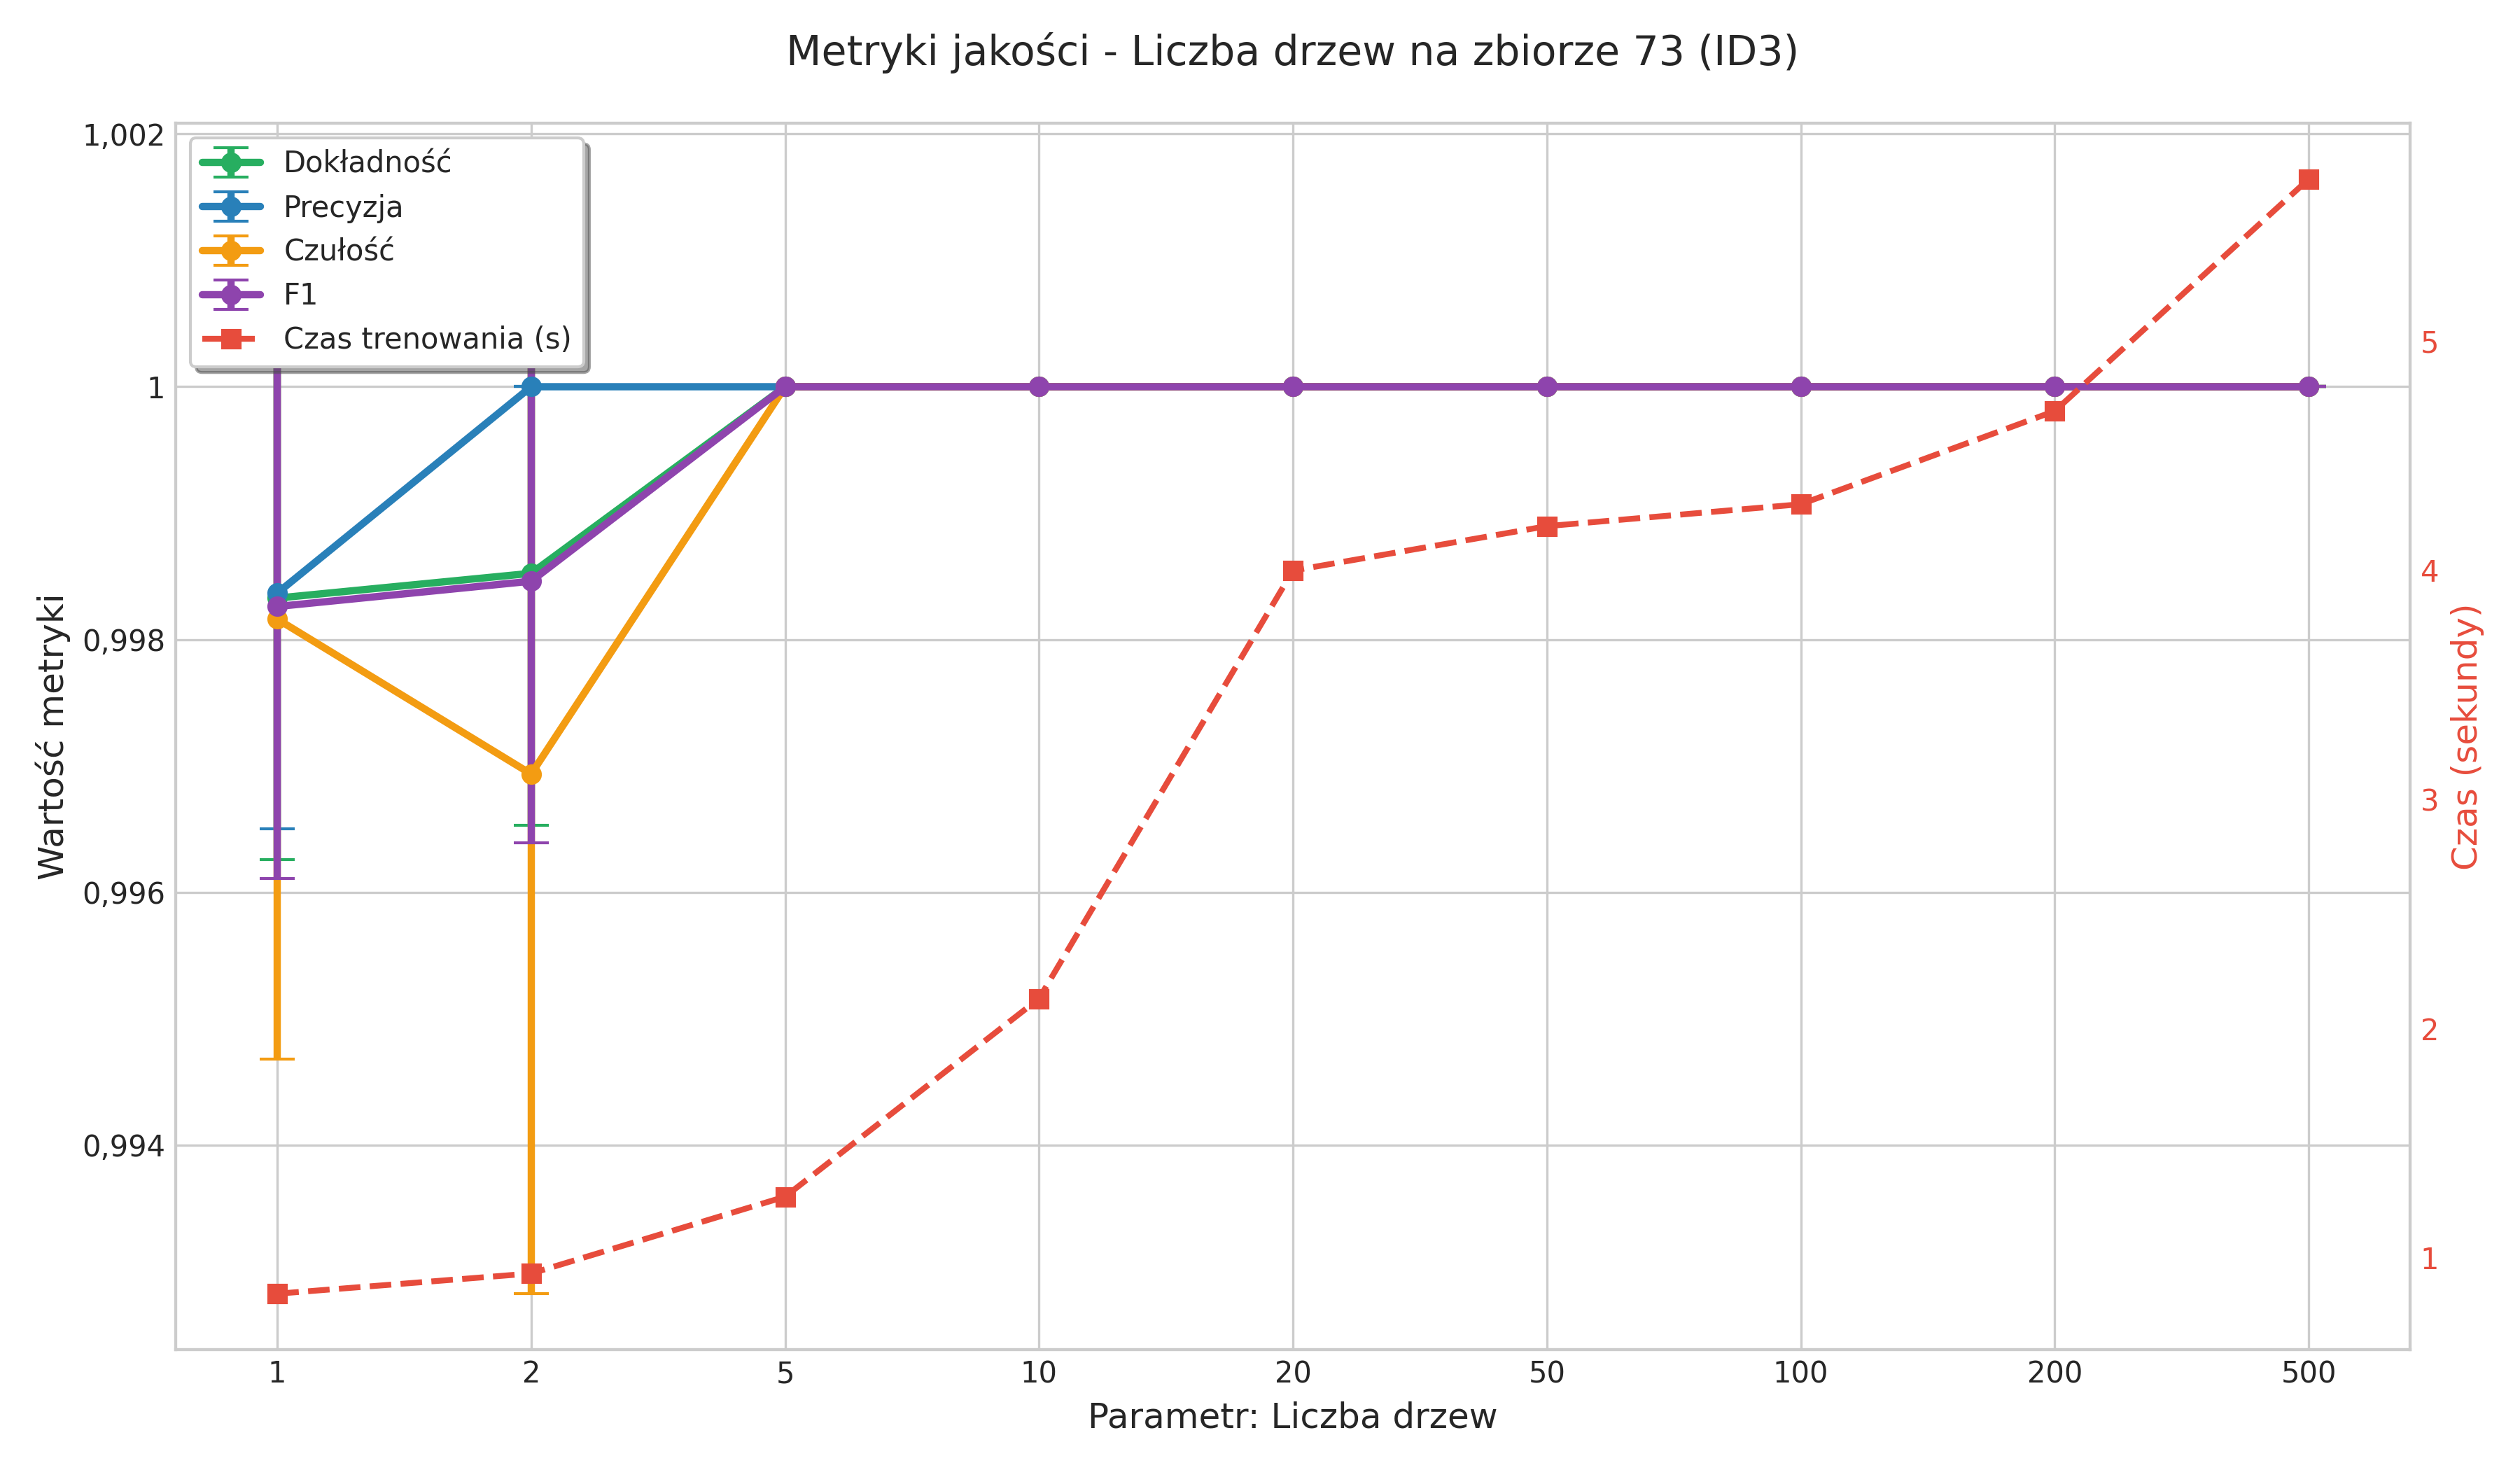
\includegraphics[width=0.9\textwidth]{plots/ID3_tree_count_73_metrics.png}
        \caption{Wpływ liczby drzew na dokładność modelu ID3 dla zbioru 73 - Grzyby.}
        \label{fig:id3_tree_count_73}
    \end{figure}

    \item Zbiór 14 - Nawrót raka piersi

    Przy trudniejszym zbiorze danych optymalne wyniki osiągane są przy liczbie drzew równej 100. Powyżej tej wartości poprawa
    jest na tyle nieznaczna, że można ją uznać za statystyczny szum.

    \begin{figure}[H]
        \centering
        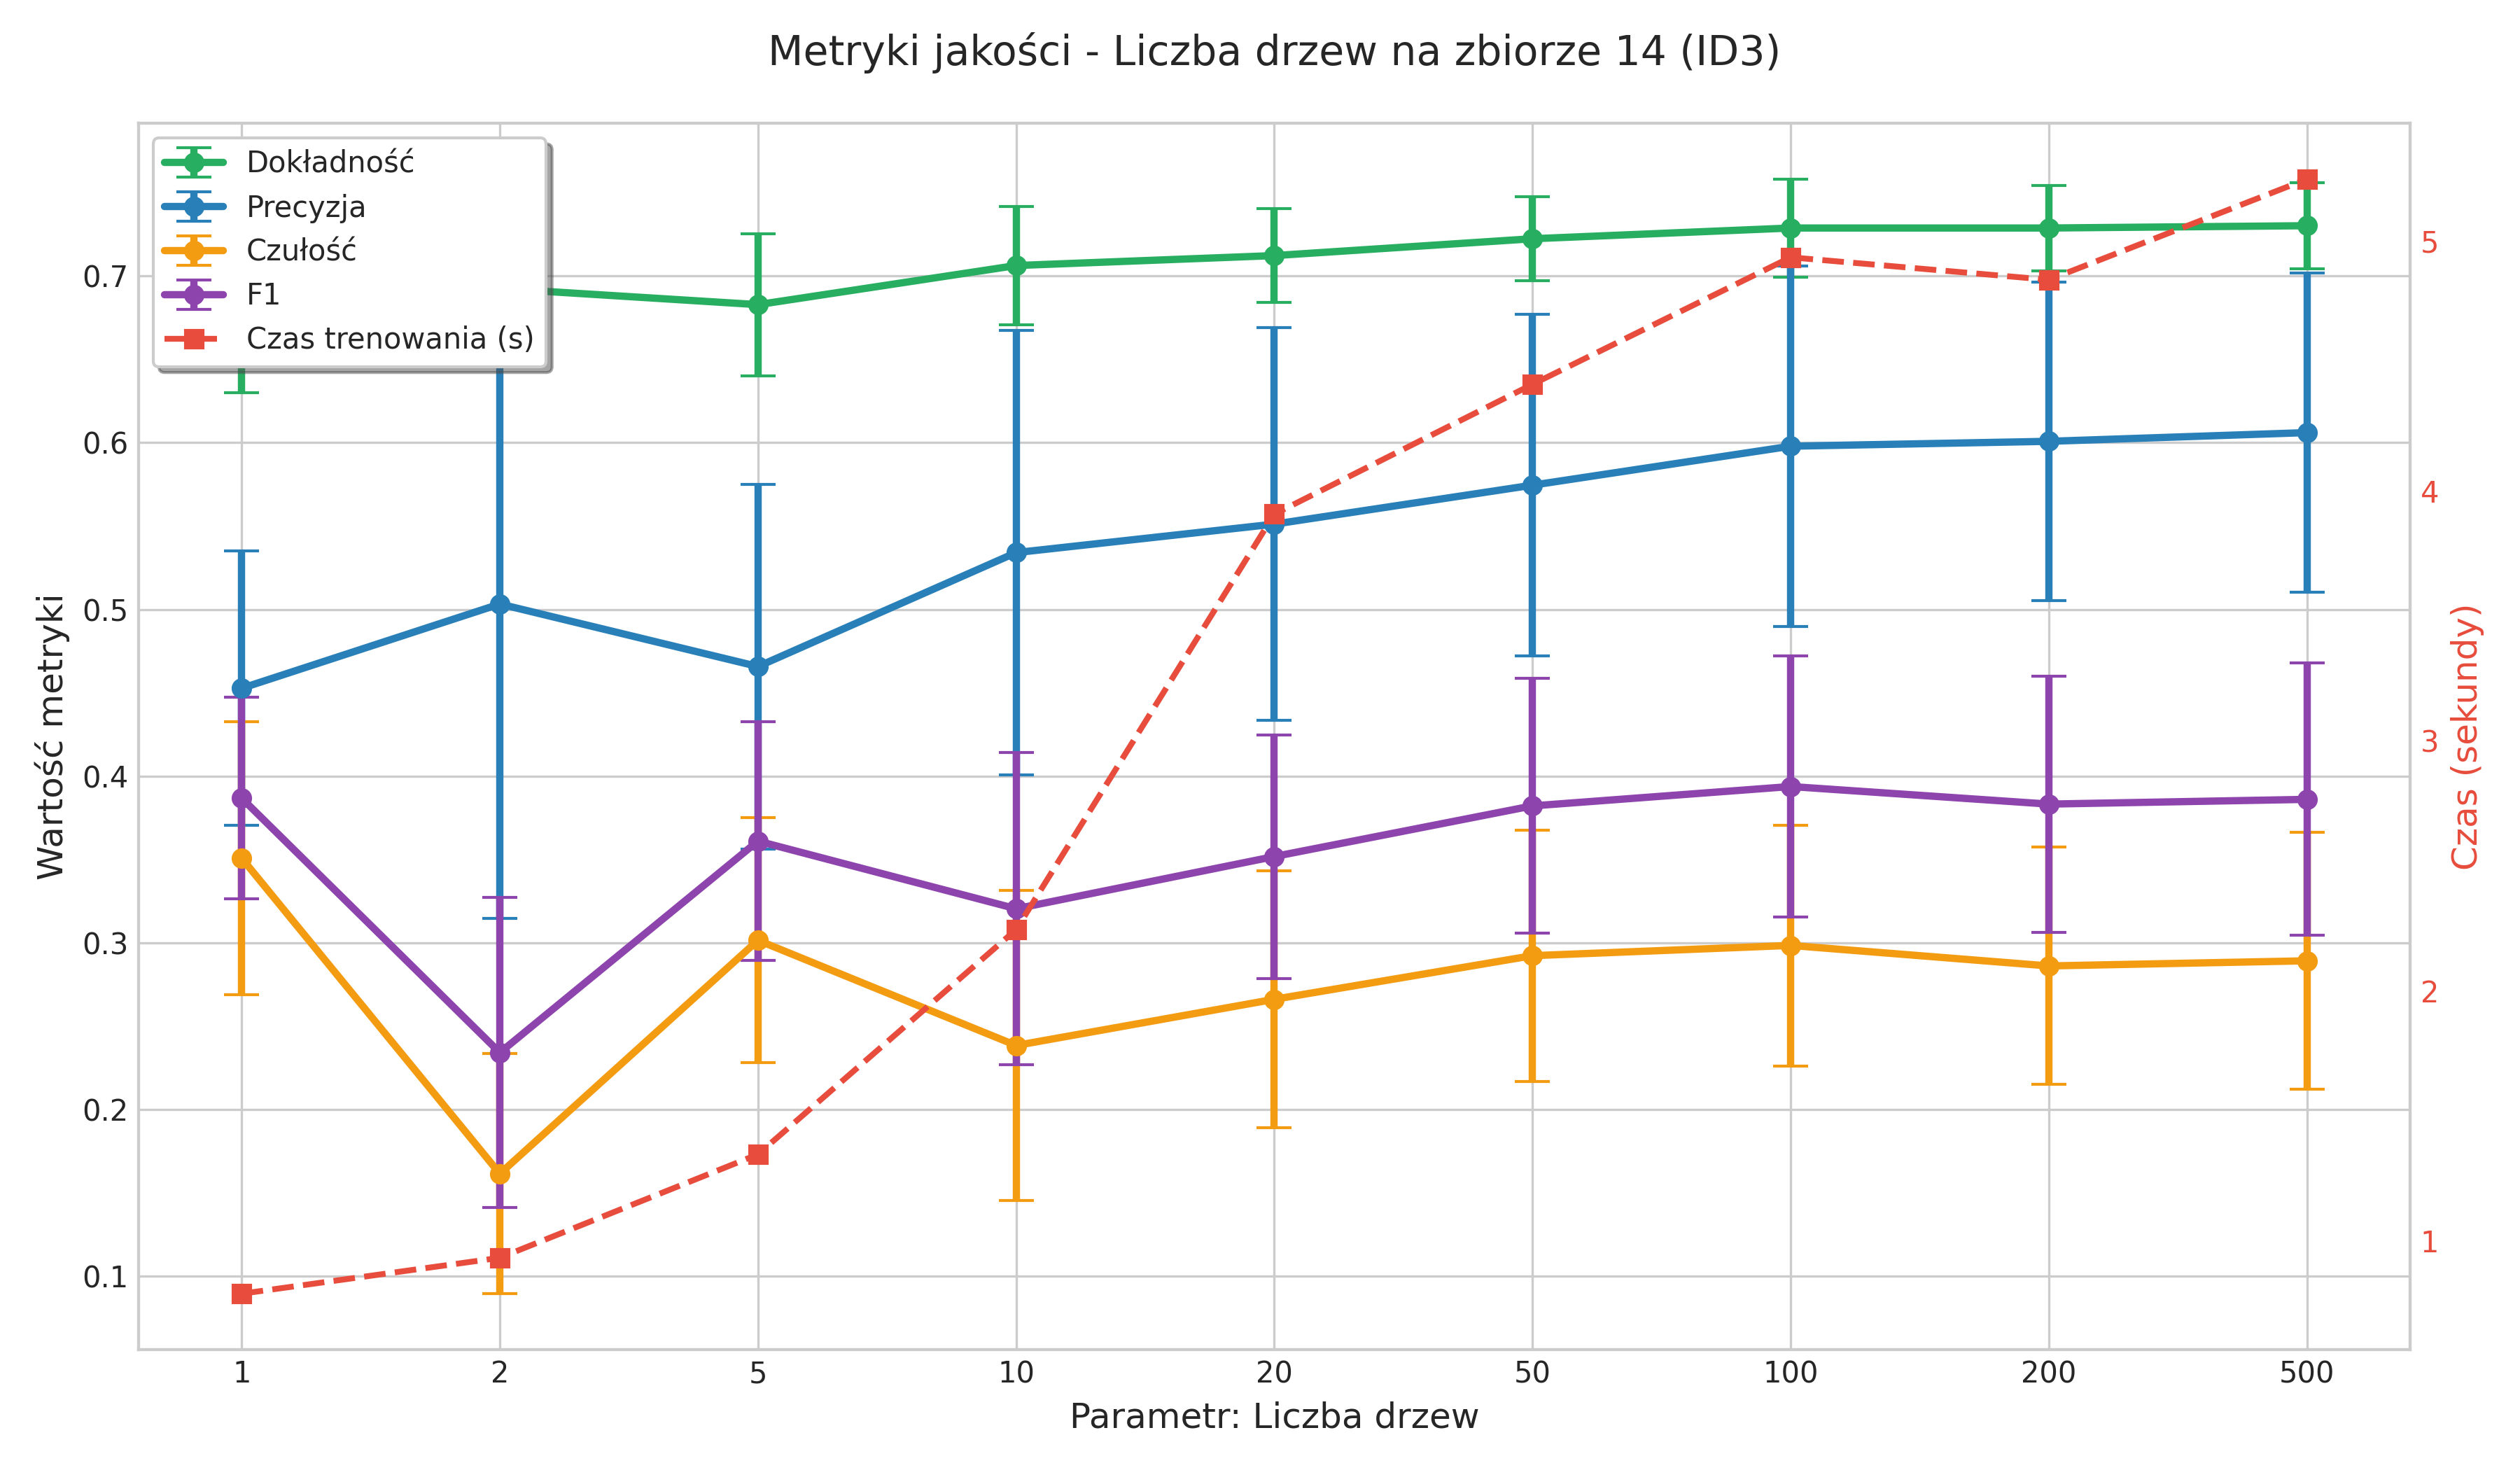
\includegraphics[width=0.9\textwidth]{plots/ID3_tree_count_14_metrics.png}
        \caption{Wpływ liczby drzew na dokładność modelu ID3 dla zbioru 14 - Nawrót raka piersi.}
        \label{fig:id3_tree_count_14}
    \end{figure}


\end{itemize}
\subsubsection{CART}

Sprawdzane wartości zostały ograniczone do maksymalnie 200 drzew ze względu na długi czas wykonywania badania.

\begin{itemize}
    \item Zbiór 73 - Grzyby

    Drzewa CART radzą sobie gorzej od ID3 - 100\% dokładności osiągają dopiero przy 50 drzewach. Wynika to z odmiennego sposobu
    kodowania atrybutów kategorycznych (one-hot encoding), które prowadzi do zwiększenia wymiarowości danych i wpływa na efektywność modelu.
    Powyżej 50 drzew miary czułości, precyzji i F1-score ulegają nieznacznej poprawie wraz ze wzrostem liczby drzew -- model jest w stanie lepiej
    radzić sobie z trudniejszymi przykładami.

    \begin{figure}[H]
        \centering
        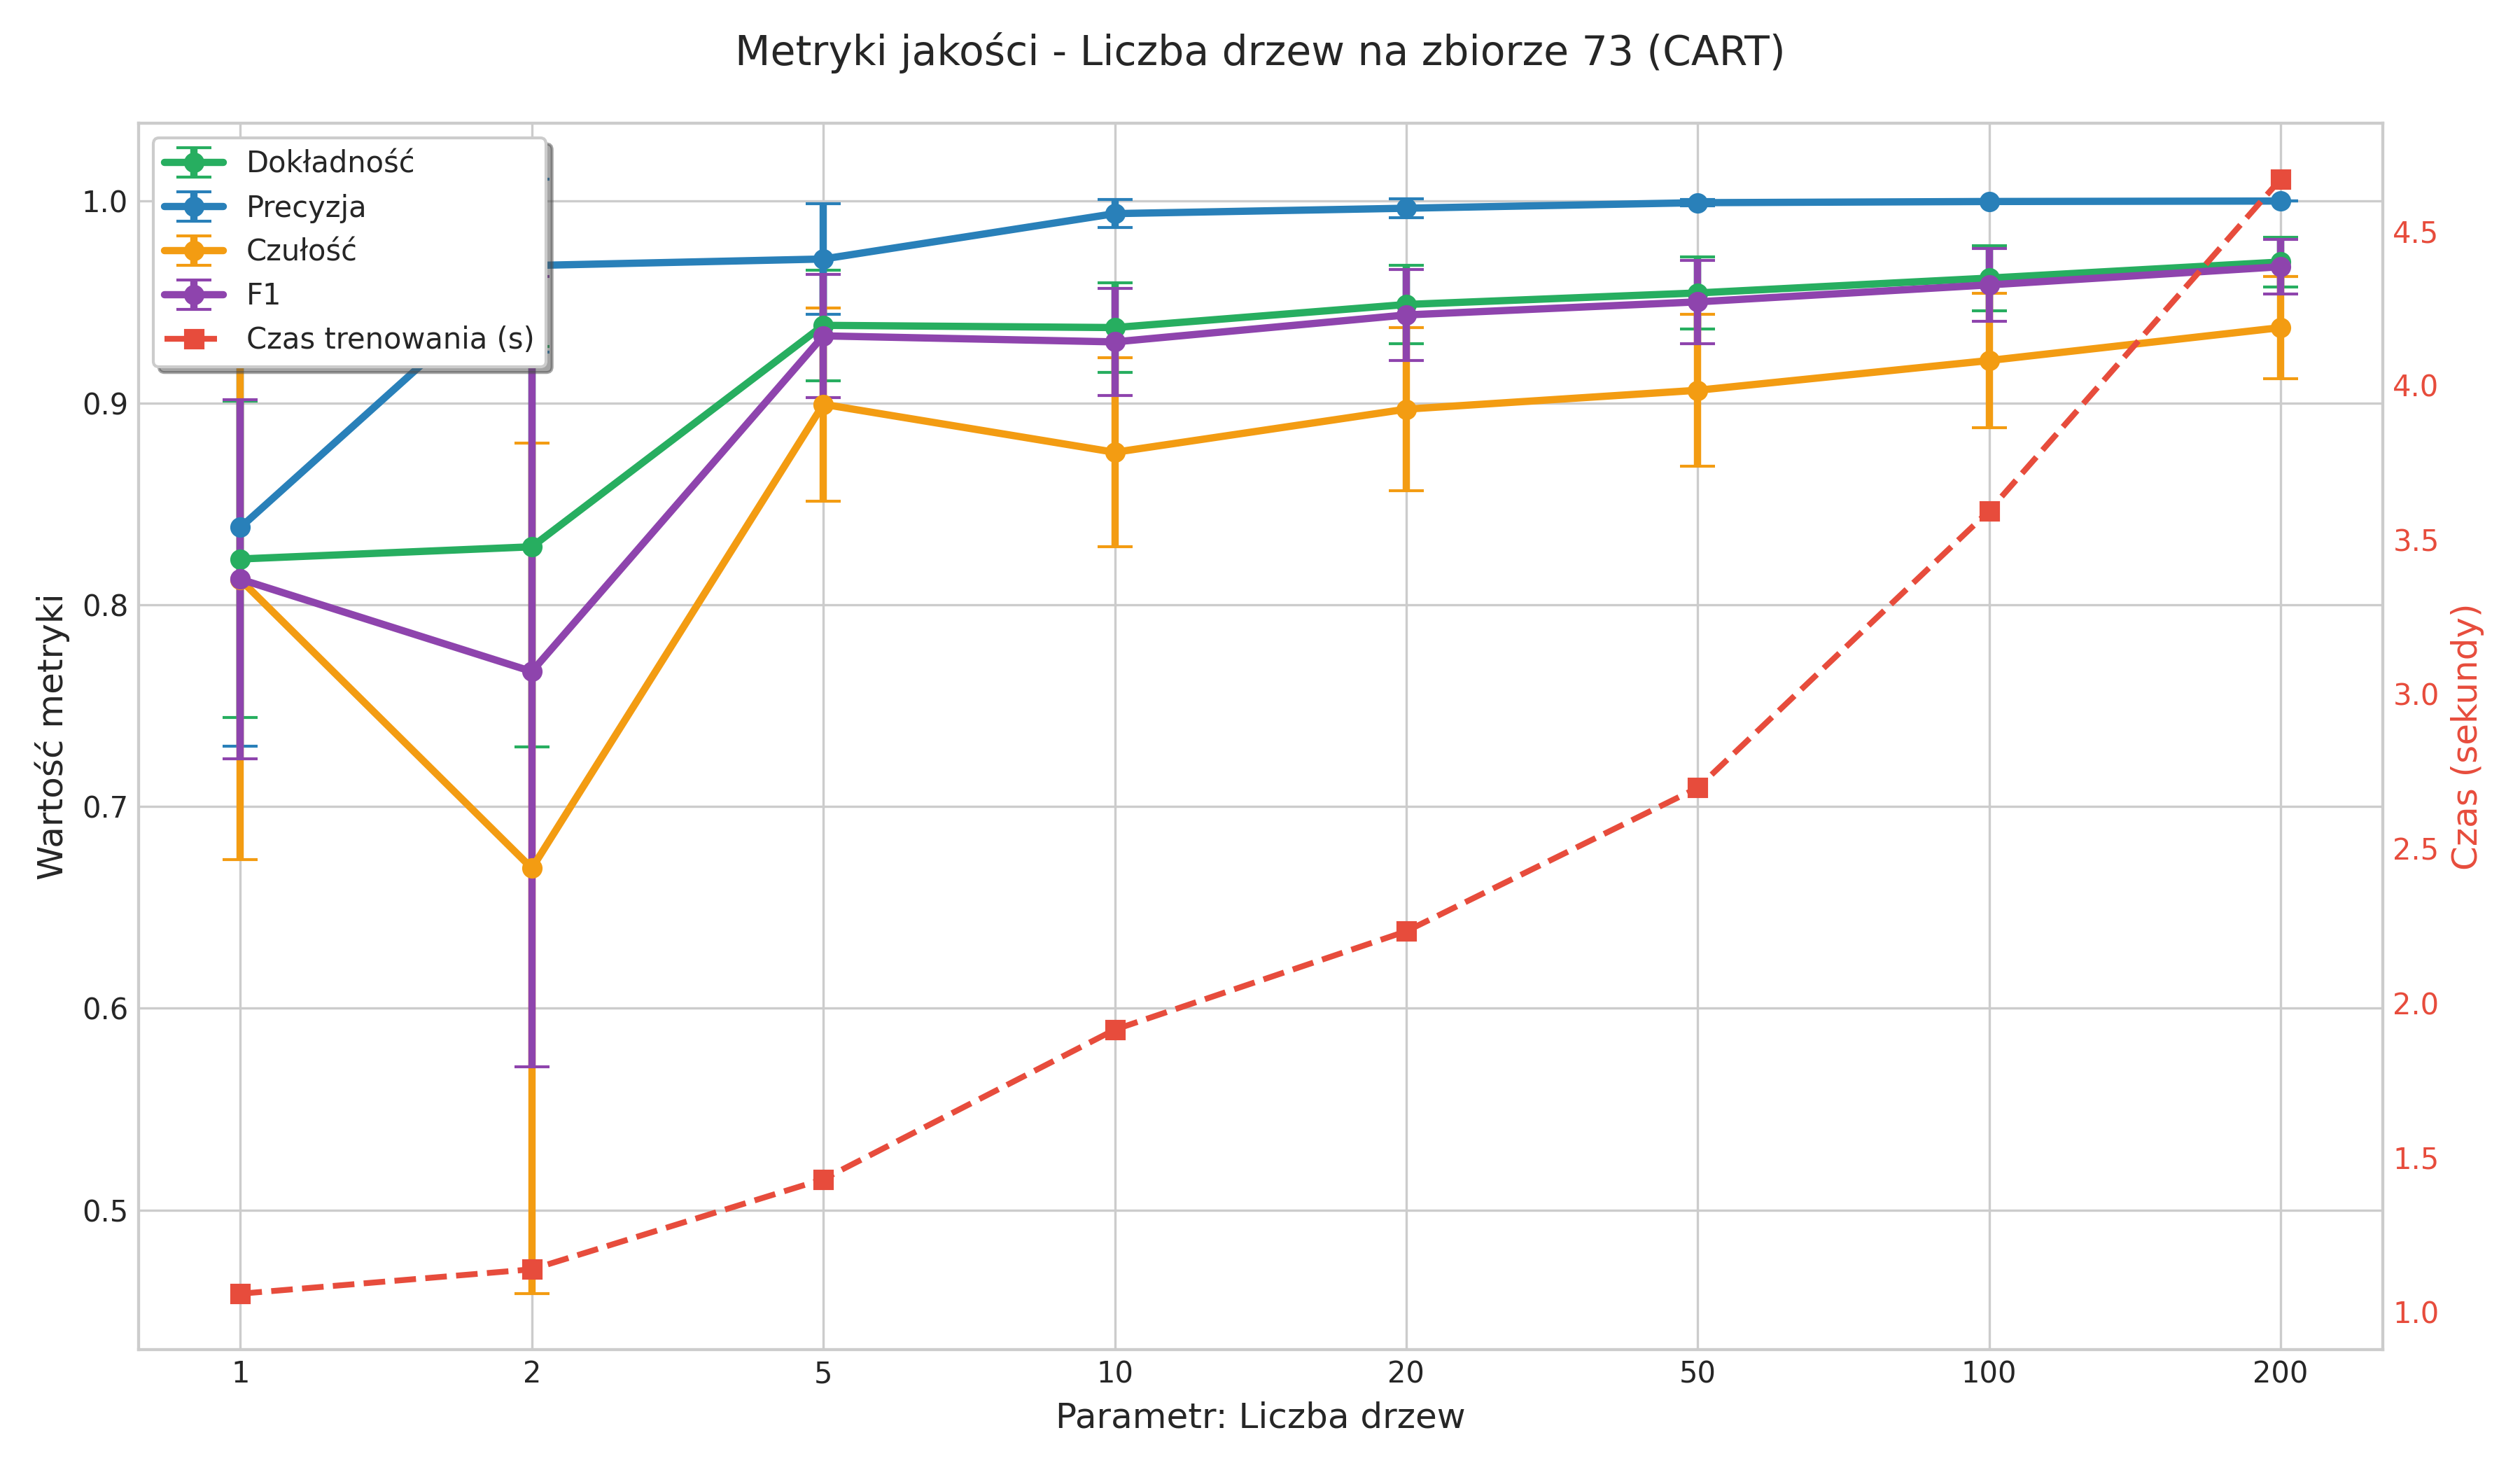
\includegraphics[width=0.9\textwidth]{plots/CART_tree_count_73_metrics.png}
        \caption{Wpływ liczby drzew na dokładność modelu CART dla zbioru 73 - Grzyby.}
        \label{fig:cart_tree_count_73}
    \end{figure}

    \item Zbiór 14 - Nawrót raka piersi

    Liczba drzew nie wpływa znacząco na dokładność, jednak do liczby 50 drzew obserwujemy wyraźną poprawę miary precyzji. Wskazuje to na
    redukcję wariancji modelu i skuteczniejszą eliminację błędów fałszywie pozytywnych (False Positives) poprzez mechanizm głosowania większościowego.

    \begin{figure}[H]
        \centering
        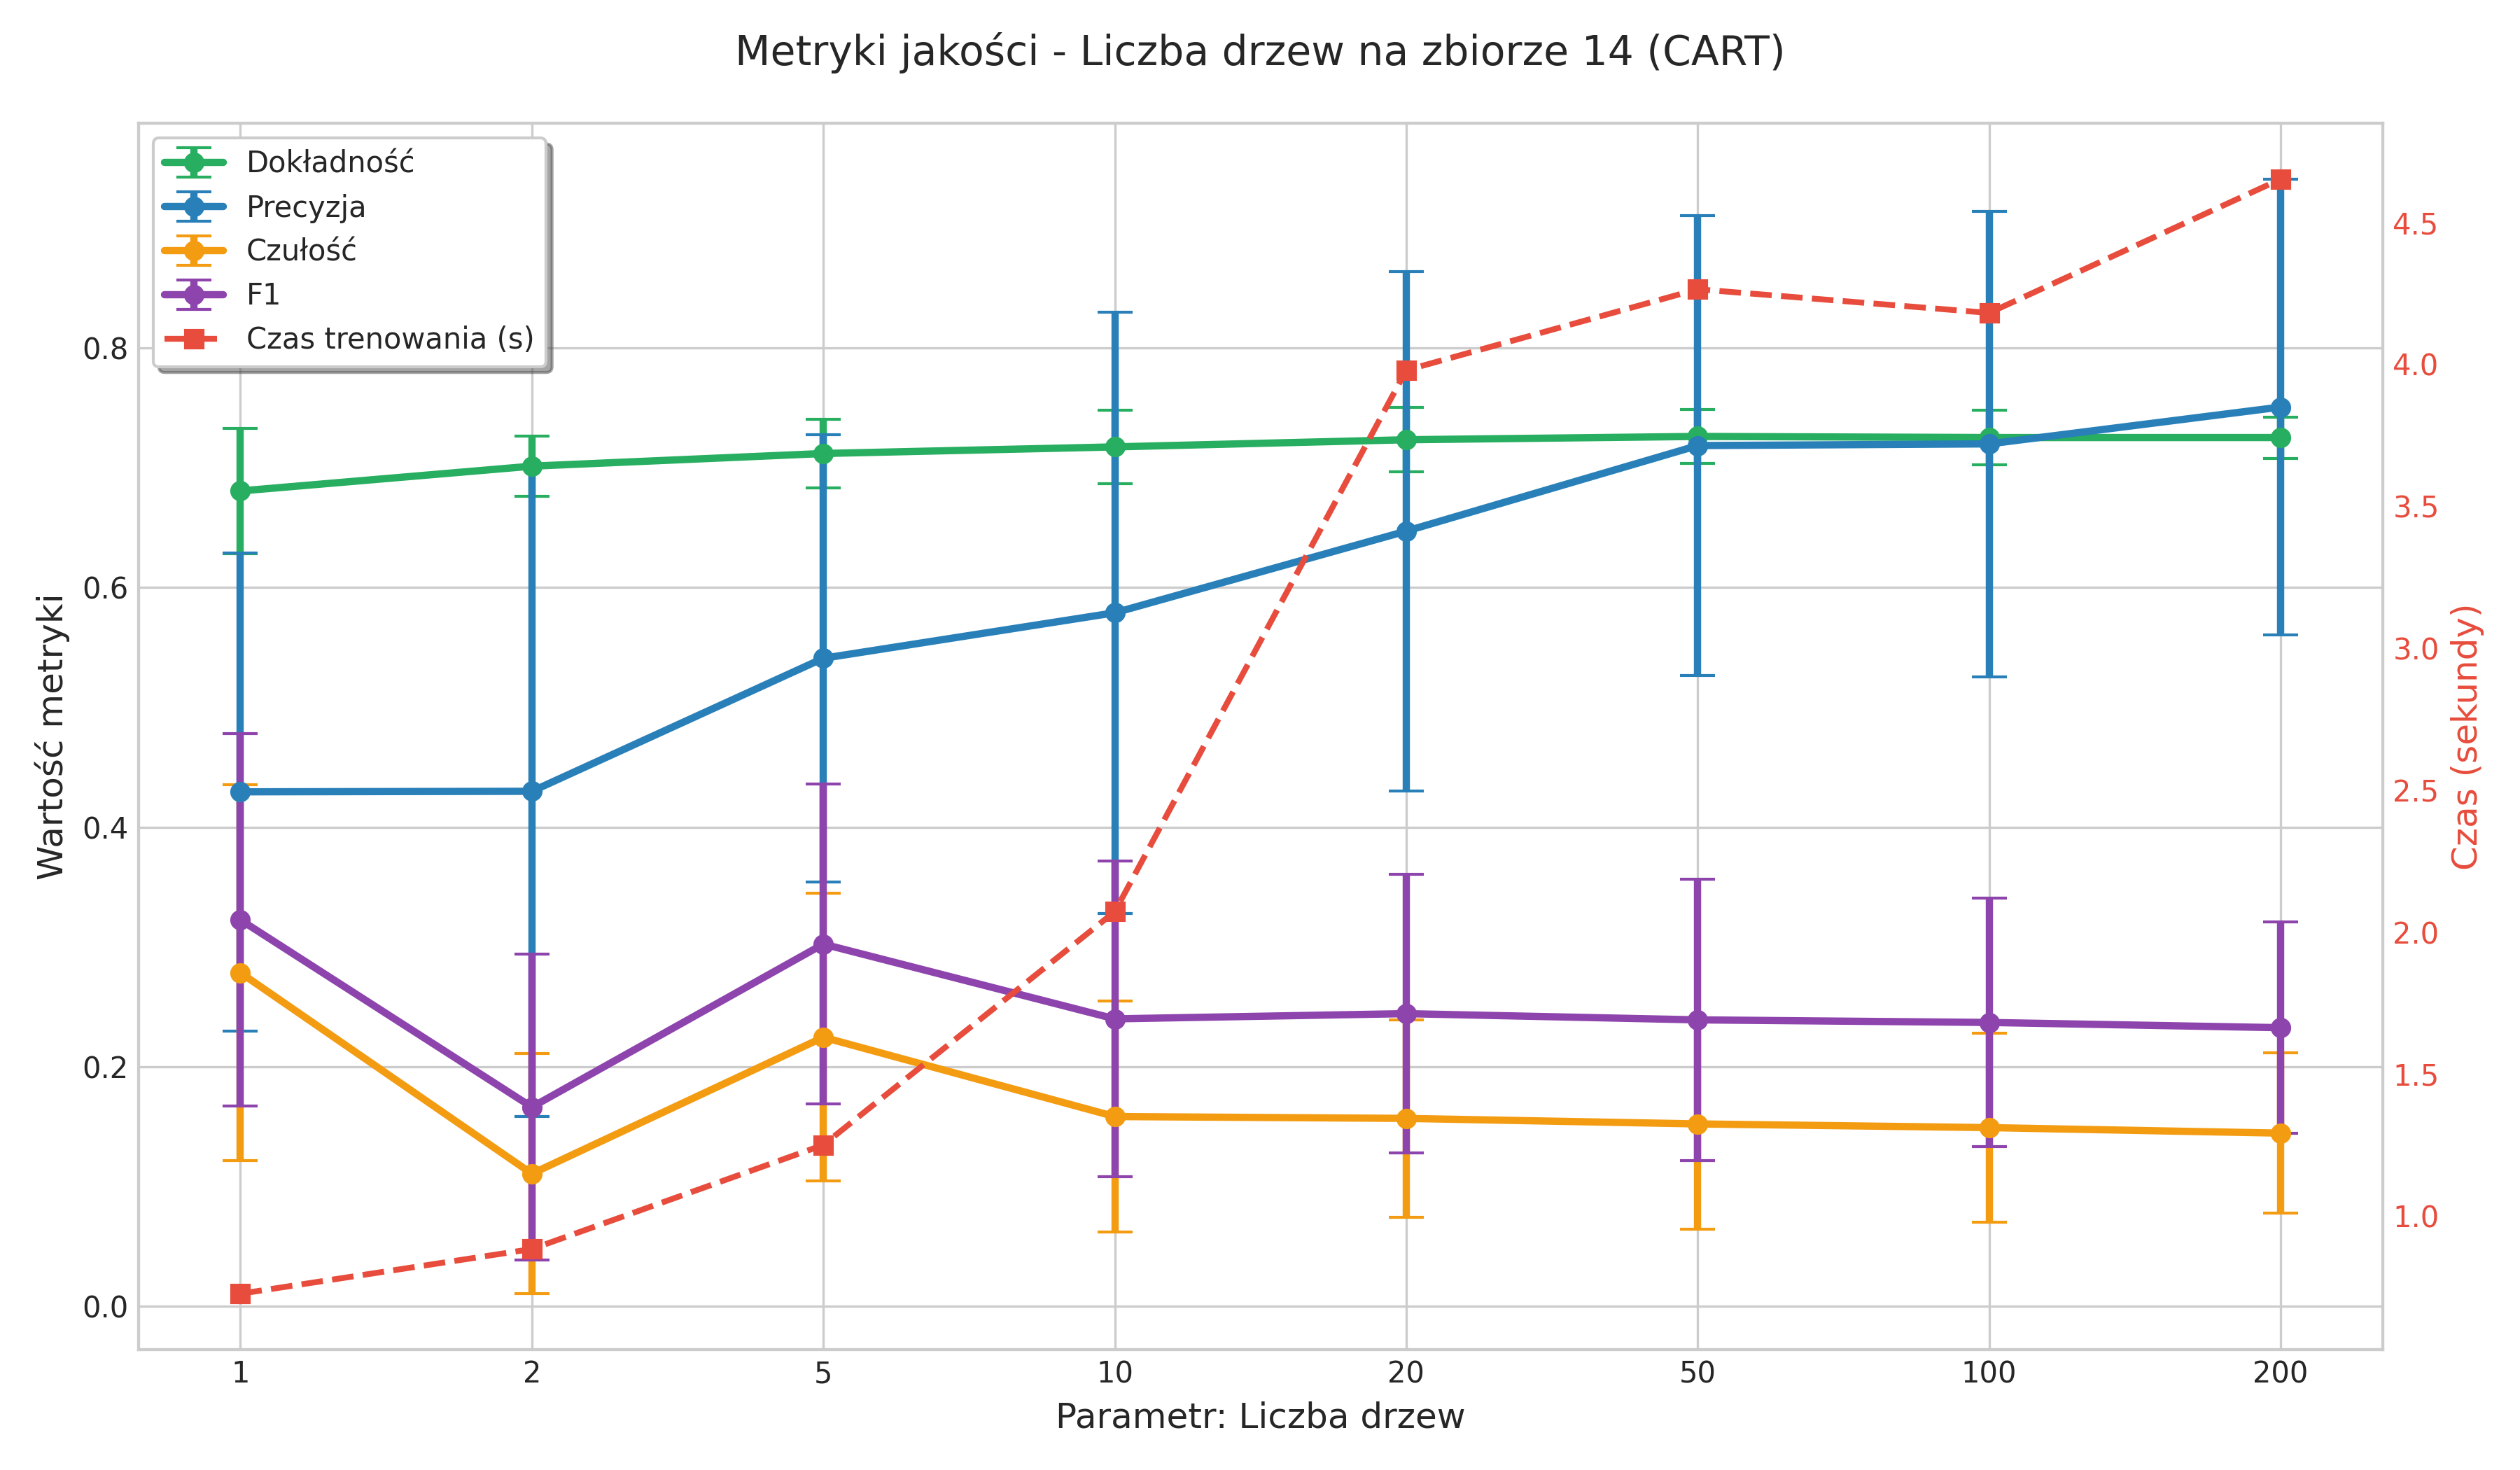
\includegraphics[width=0.9\textwidth]{plots/CART_tree_count_14_metrics.png}
        \caption{Wpływ liczby drzew na dokładność modelu CART dla zbioru 14 - Nawrót raka piersi.}
        \label{fig:cart_tree_count_14}
    \end{figure}

    \item Zbiór 222 - Skuteczność marketingu bankowego

    Obserwacje oraz wnioski są podobne jak dla zbioru 14. Liczba drzew powyżej 50 nie wpływa znacząco na dokładność, jednak
    do tej wartości widoczna jest poprawa precyzji modelu. Warto zauważyć również bardzo niskie poziomy czułości oraz F1-score, które
    wskazują na trudność zbioru danych. Algorytm ma problem z wykryciem klasy pozytywnej i w znacznej liczbie przypadków działa podobnie
    jak klasyfikator naiwny zawsze przewidujący klasę negatywną.

    \begin{figure}[H]
        \centering
        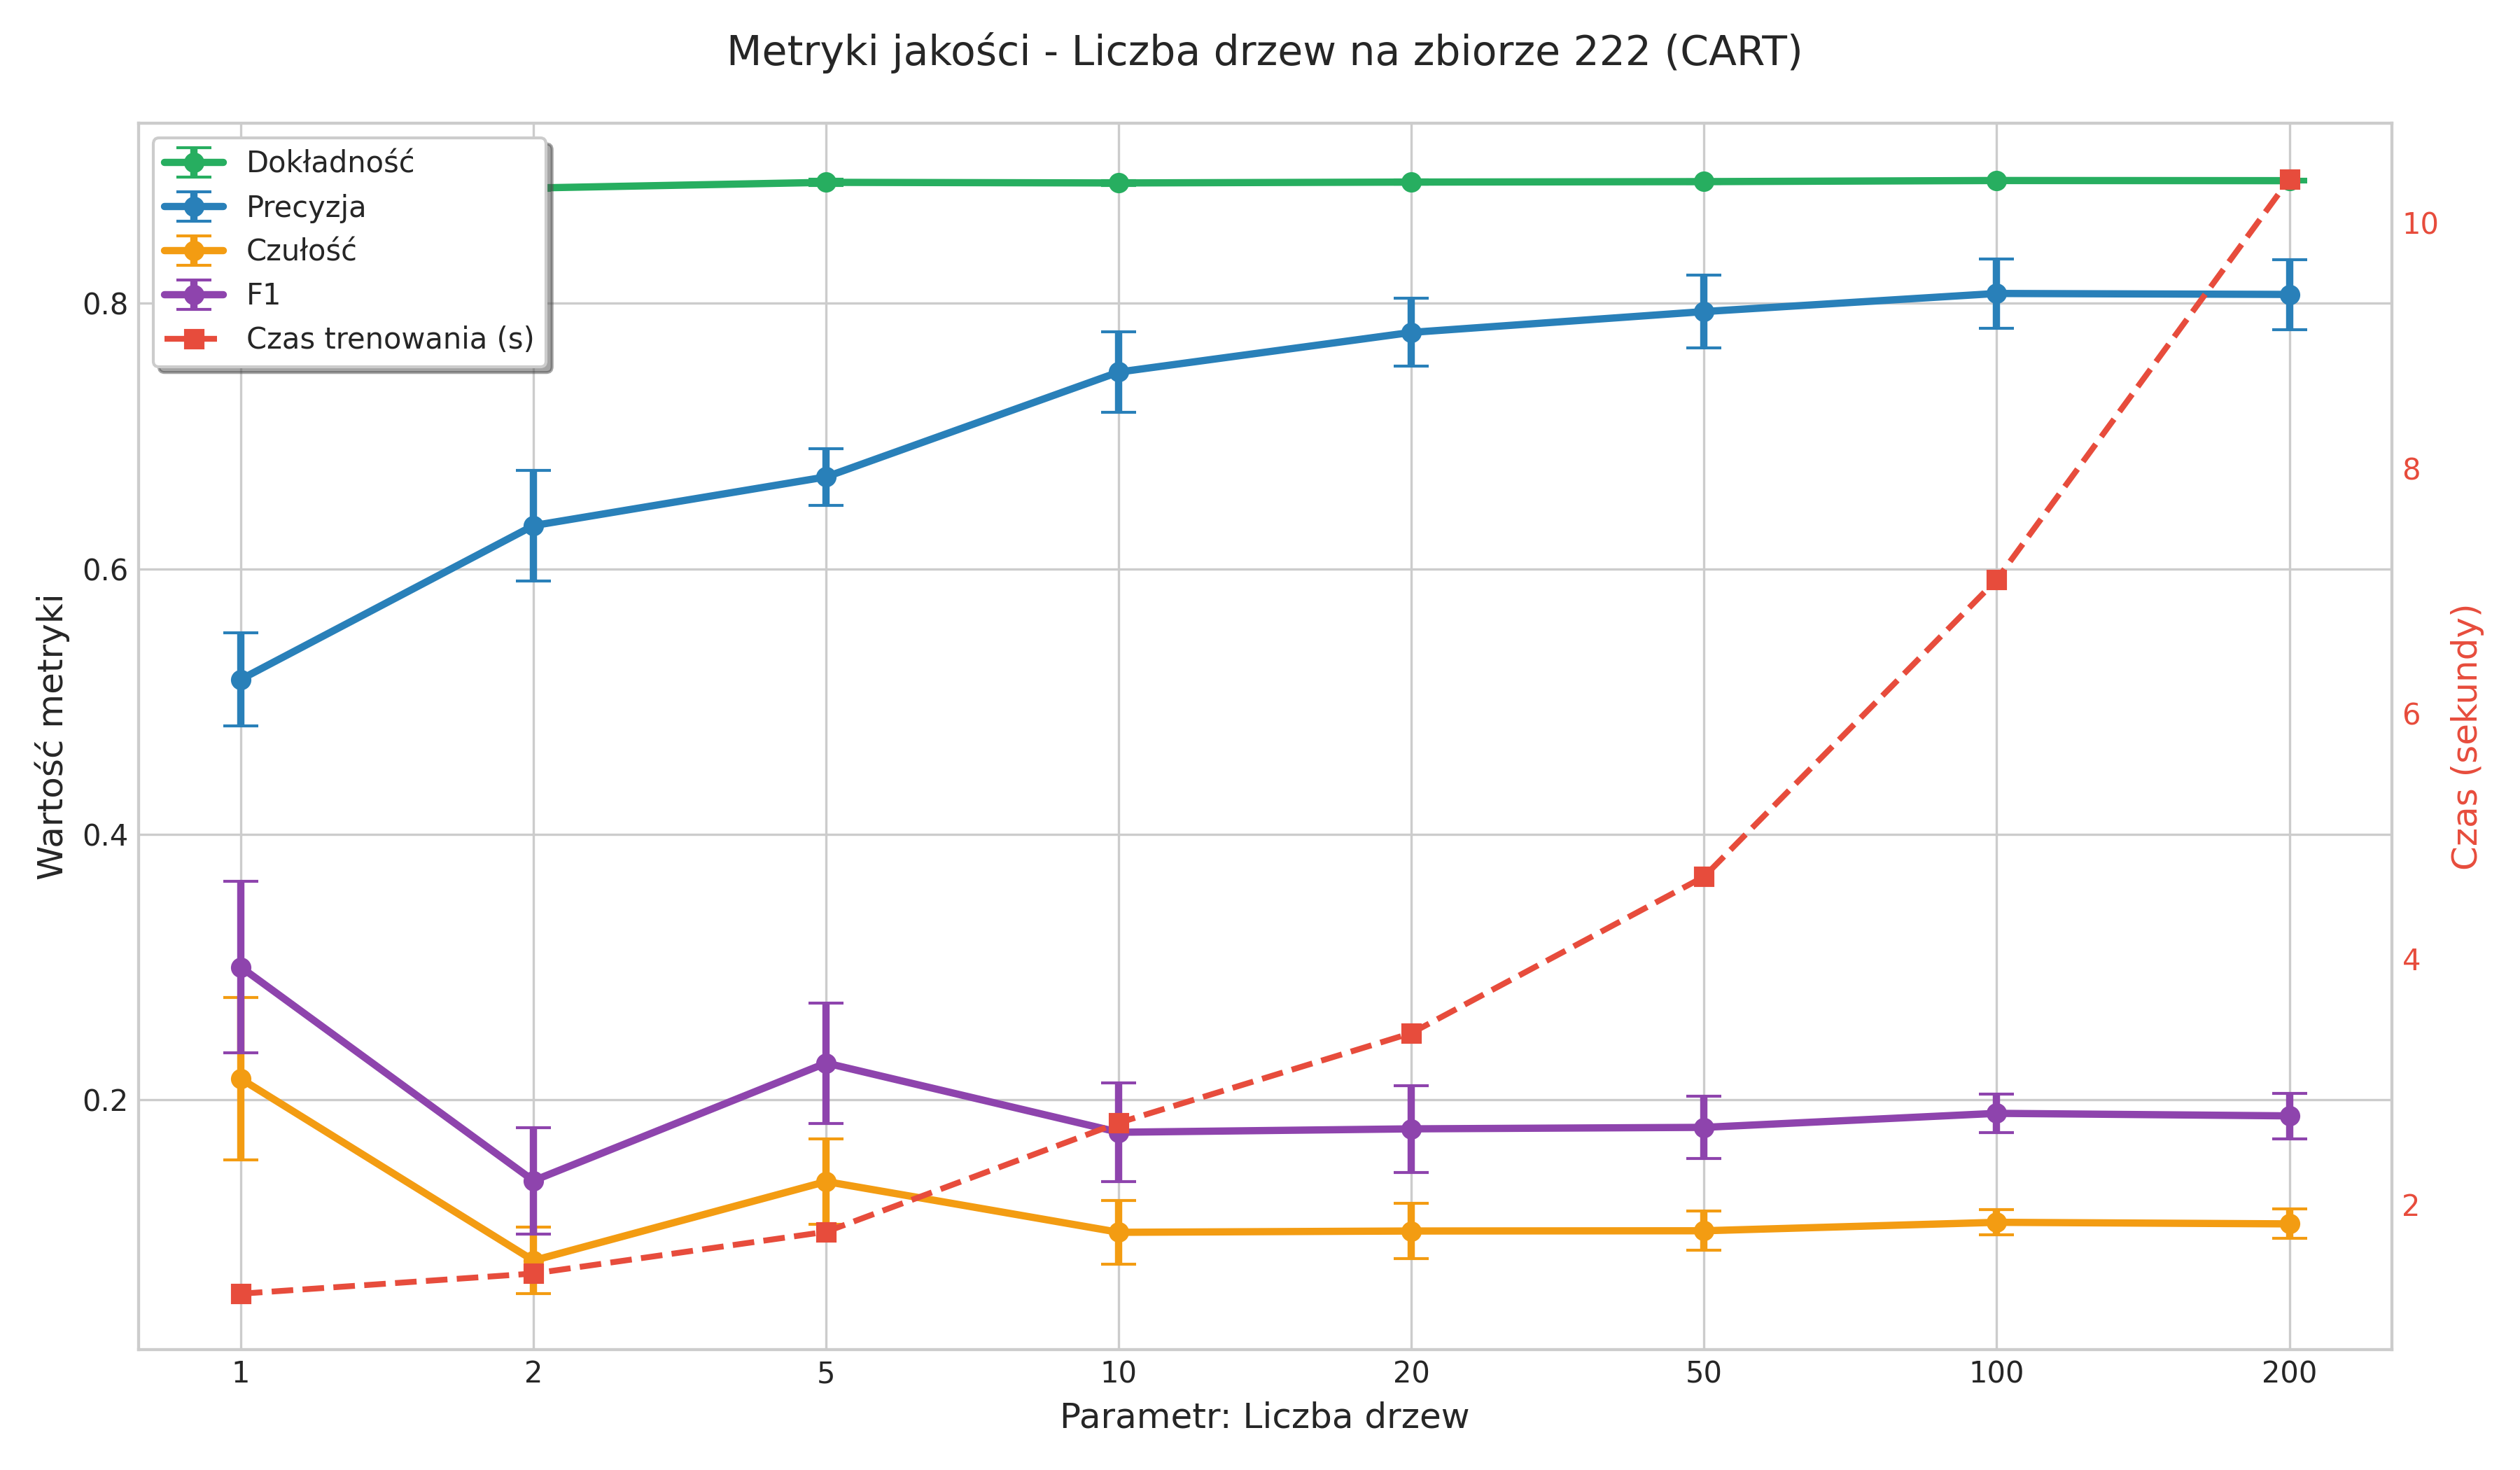
\includegraphics[width=0.9\textwidth]{plots/CART_tree_count_222_metrics.png}
        \caption{Wpływ liczby drzew na dokładność modelu CART dla zbioru 222 - Skuteczność marketingu bankowego.}
        \label{fig:cart_tree_count_222}
    \end{figure}

    \item Zbiór 350 - Zaległości płatnicze klientów kart kredytowych

    Na tym zbiorze wzrost liczby drzew wpływa nie tylko na poprawę precyzji modelu, ale też czułość oraz F1-score. Oznacza to, że
    zwiększenie liczby drzew pozwala na redukcję zarówno błędów fałszywie pozytywnych (False Positives), jak i fałszywie negatywnych (False Negatives).
    Wpływ na dokładność jest jednak niewielki.

    \begin{figure}[H]
        \centering
        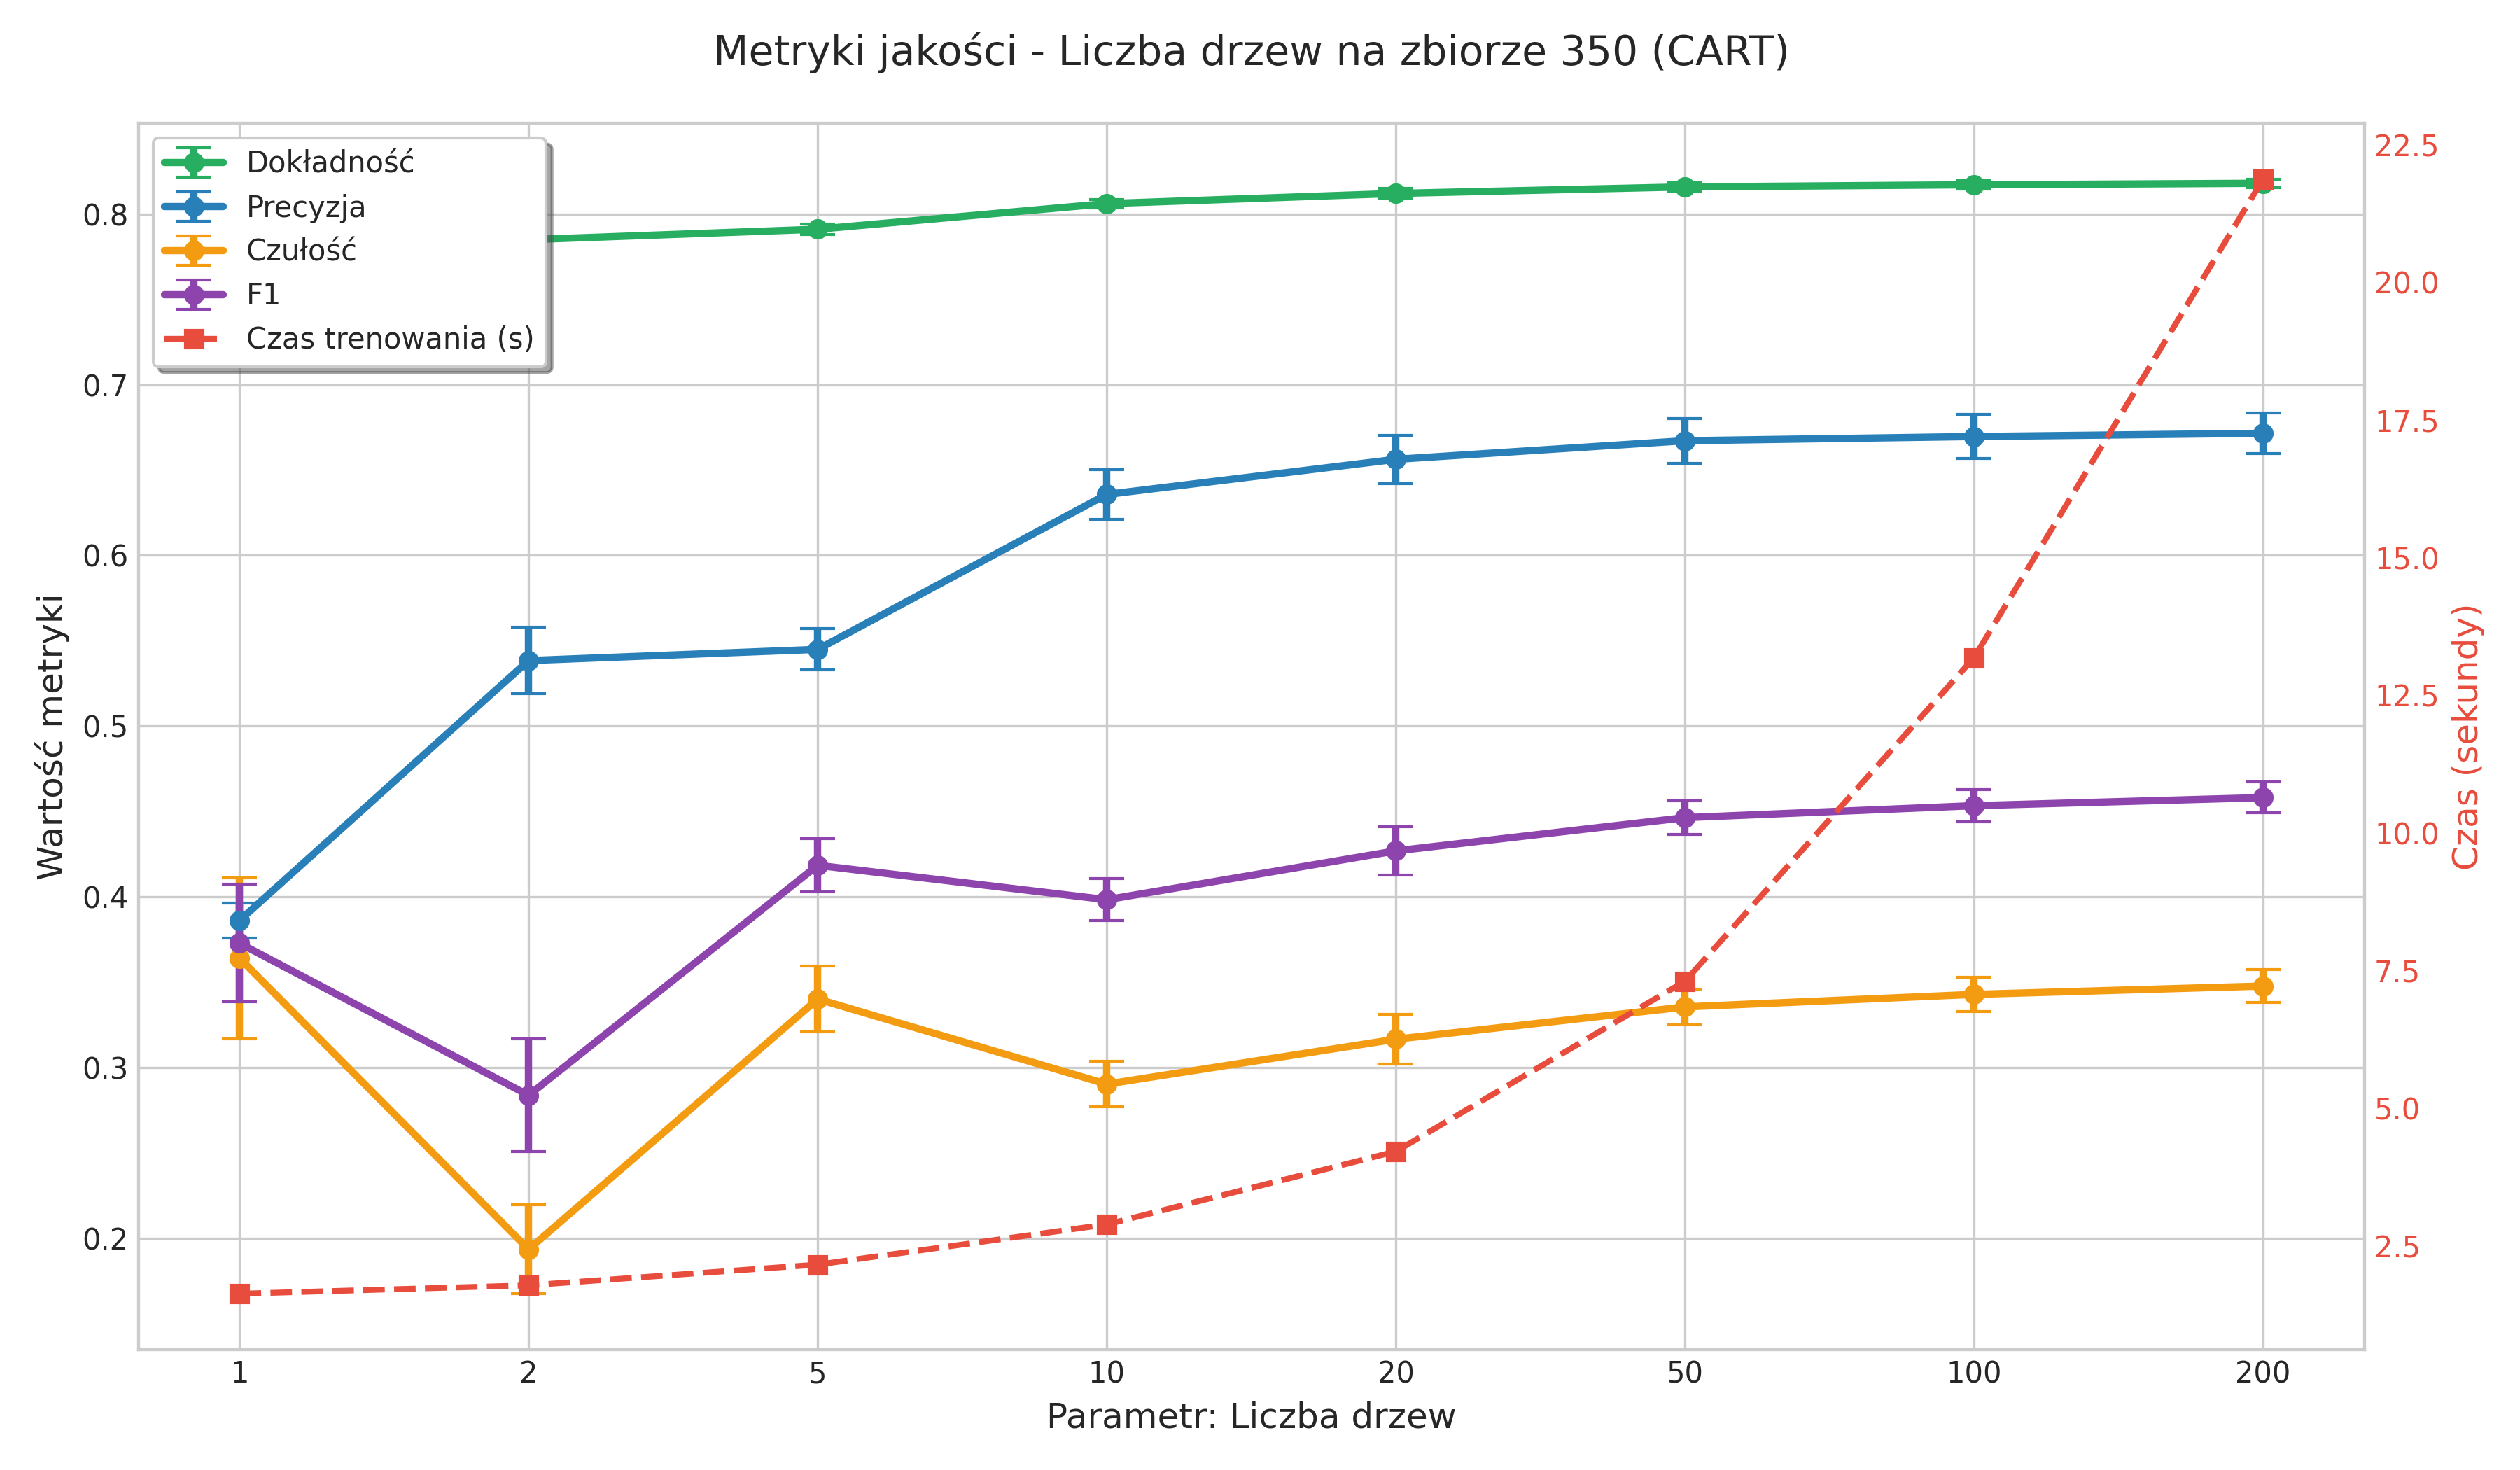
\includegraphics[width=0.9\textwidth]{plots/CART_tree_count_350_metrics.png}
        \caption{Wpływ liczby drzew na dokładność modelu CART dla zbioru 350 - Zaległości płatnicze klientów kart kredytowych.}
        \label{fig:cart_tree_count_350}
    \end{figure}
\end{itemize}

\subsubsection{Wnioski ogólne}

\begin{itemize}
    \item Uzasadnionym jest stosowanie lasu losowego o liczbie drzew równej co najmniej 50, gdyż pozwala to na stabilizację wyników i redukcję wariancji modelu.
    \item W porównywaniu modeli zostanie utrzymana liczba drzew w lesie równa 100.
\end{itemize}


\subsection{Współczynnik próbkowania zbioru trenującego}

Współczynnik próbkowania określa, jak dużą część zbioru trenującego wykorzystujemy do budowy pojedynczego drzewa w lesie.
Jego mniejsze wartości zwiększają różnorodność drzew, co może prowadzić do redukcji zjawiska przeuczania.
Z drugiej strony przy małych zbiorach danych może prowadzić do niedouczenia poszczególnych drzew.

\subsubsection{ID3}
\begin{itemize}
    \item Zbiór 73 - Grzyby

    Wyniki są stabilne i osiągają 100\% dokładności od współczynnika równego 40\%. Odchylenia dla wartości 20\% wynikają z faktu, iż
    przy tak małej próbce rozkład klas w zbiorze trenującym może nie być reprezentatywny.

    \begin{figure}[H]
        \centering
        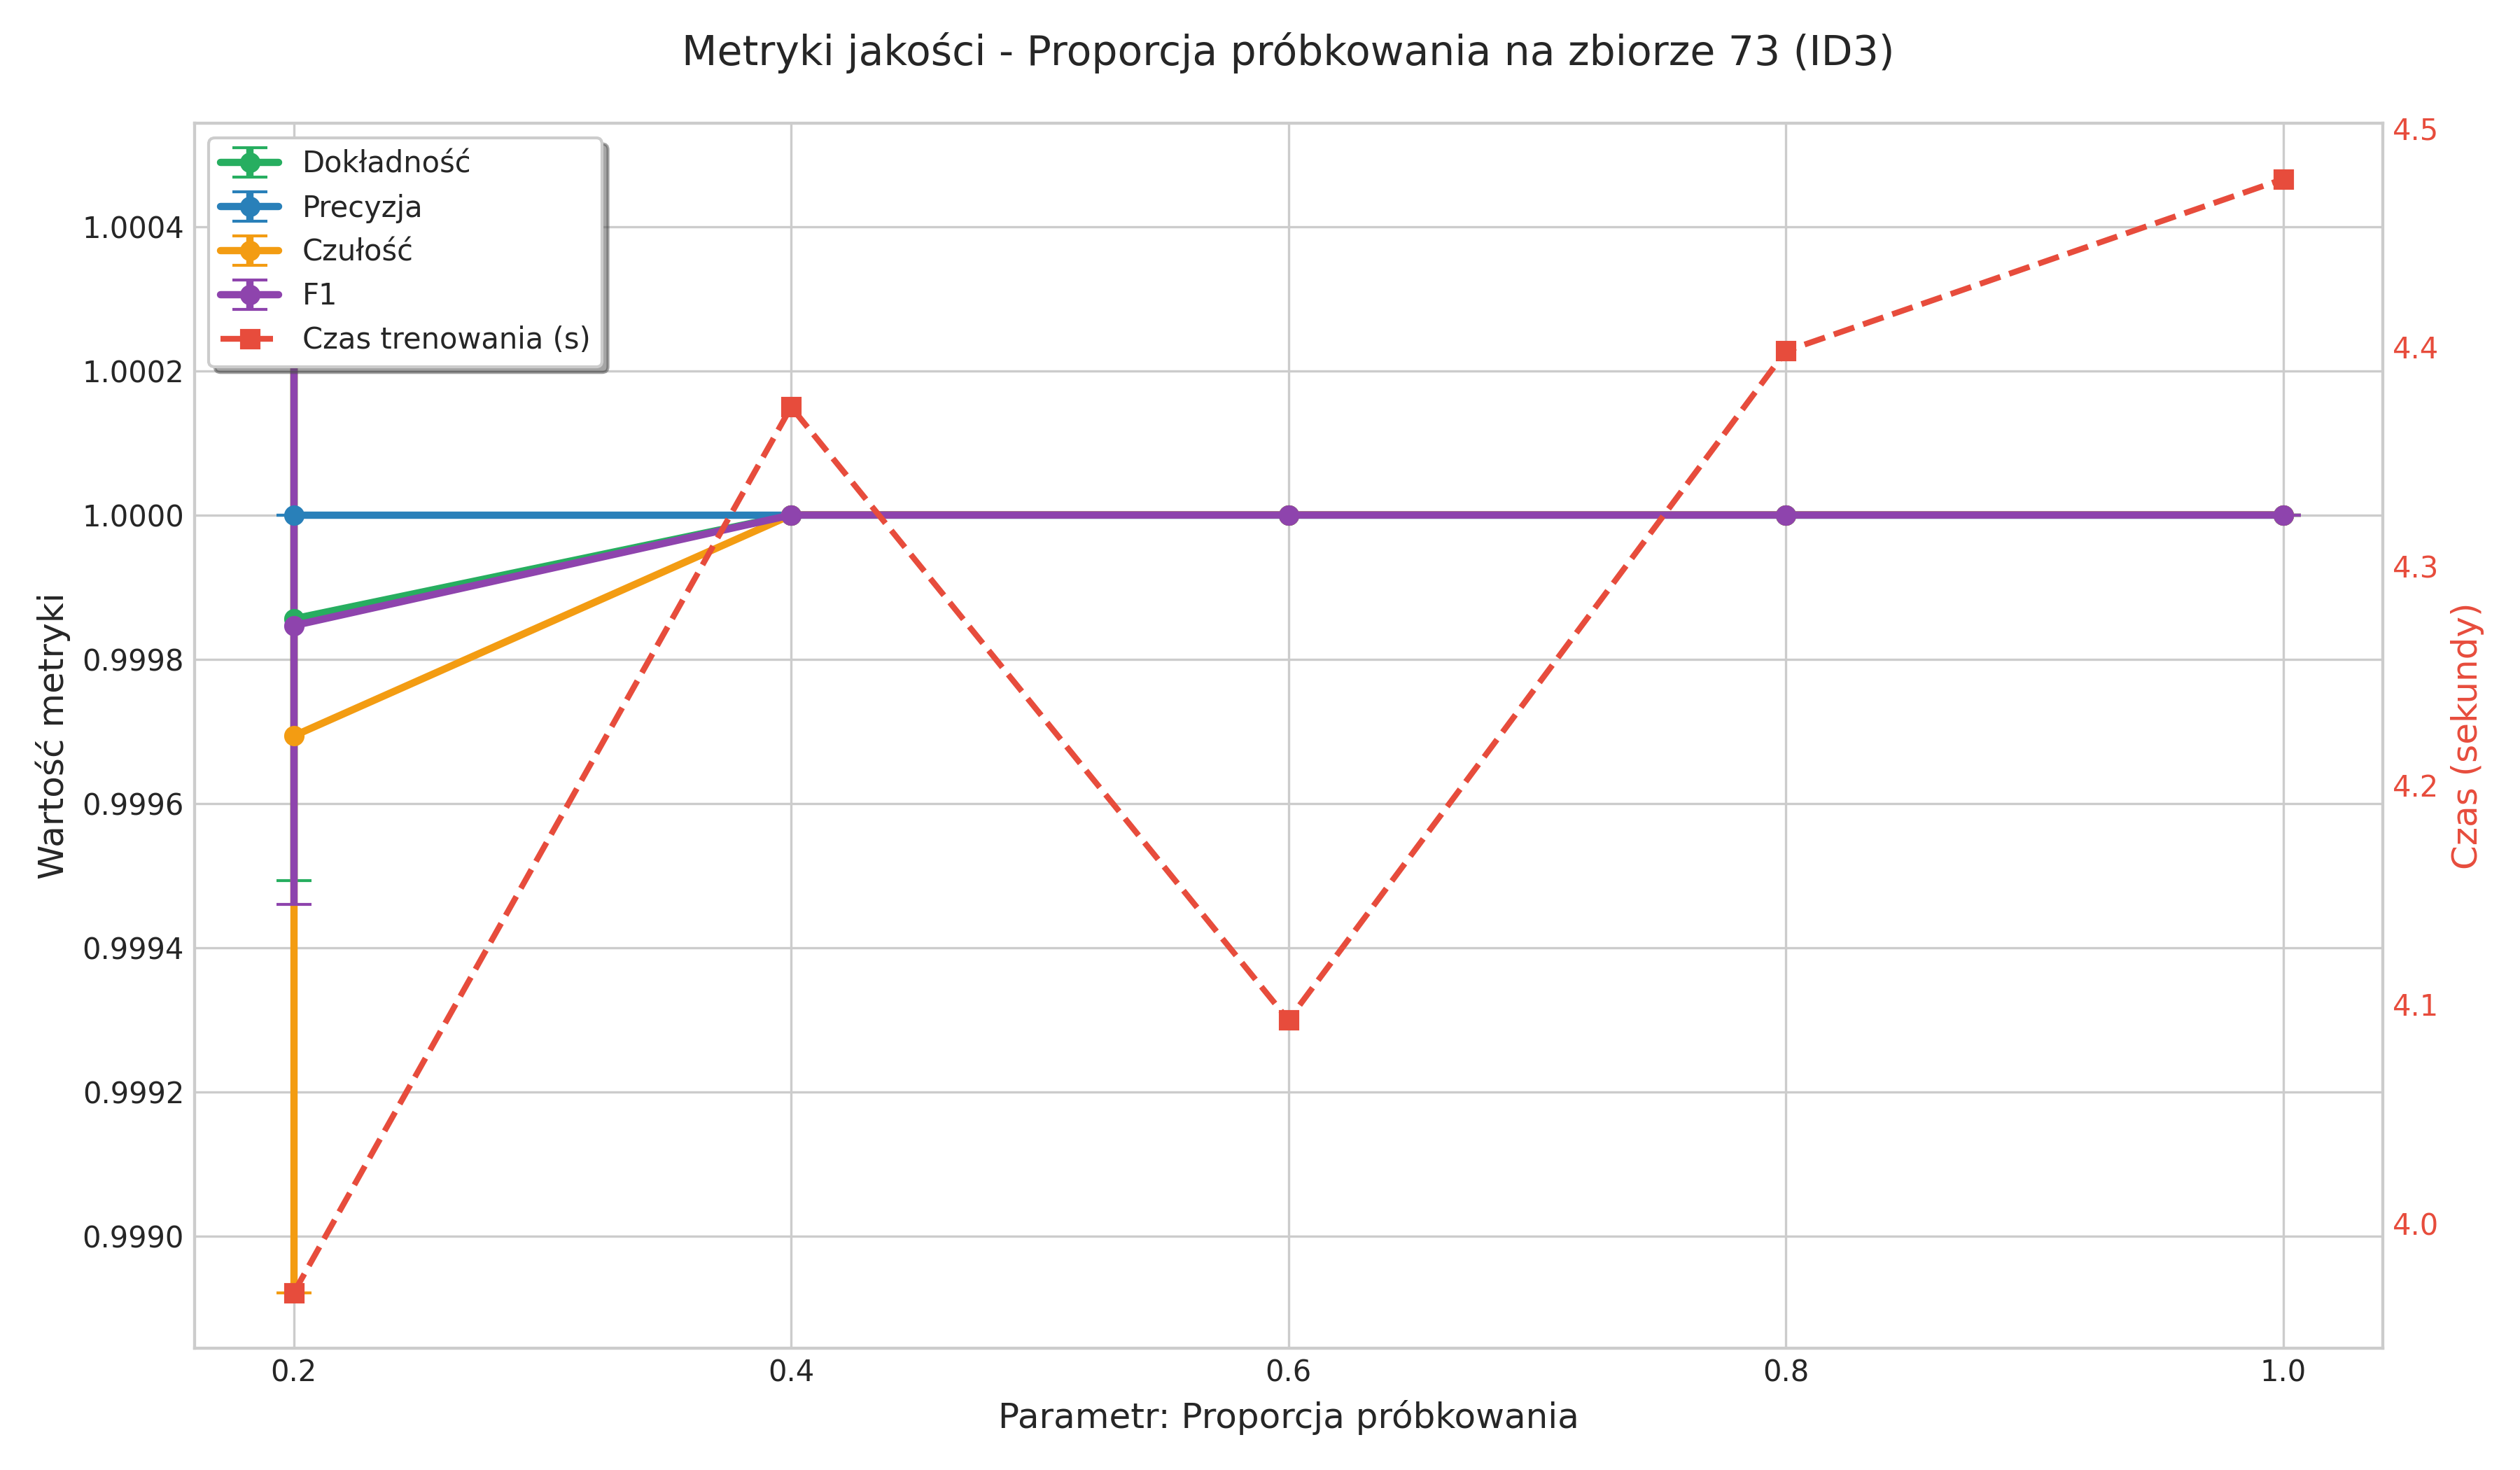
\includegraphics[width=0.9\textwidth]{plots/ID3_sample_ratio_73_metrics.png}
        \caption{Wpływ współczynnika próbkowania na dokładność modelu ID3 dla zbioru 73 - Grzyby.}
        \label{fig:id3_sample_ratio_73}
    \end{figure}

    \item Zbiór 14 - Nawrót raka piersi

    Ten zbiór danych posiada niewiele przykładów, co sprawia, że zbyt mały współczynnik próbkowania prowadzi do niedouczenia drzew.
    Optymalne wyniki osiągane są przy współczynniku równym 100\%.

    \begin{figure}[H]
        \centering
        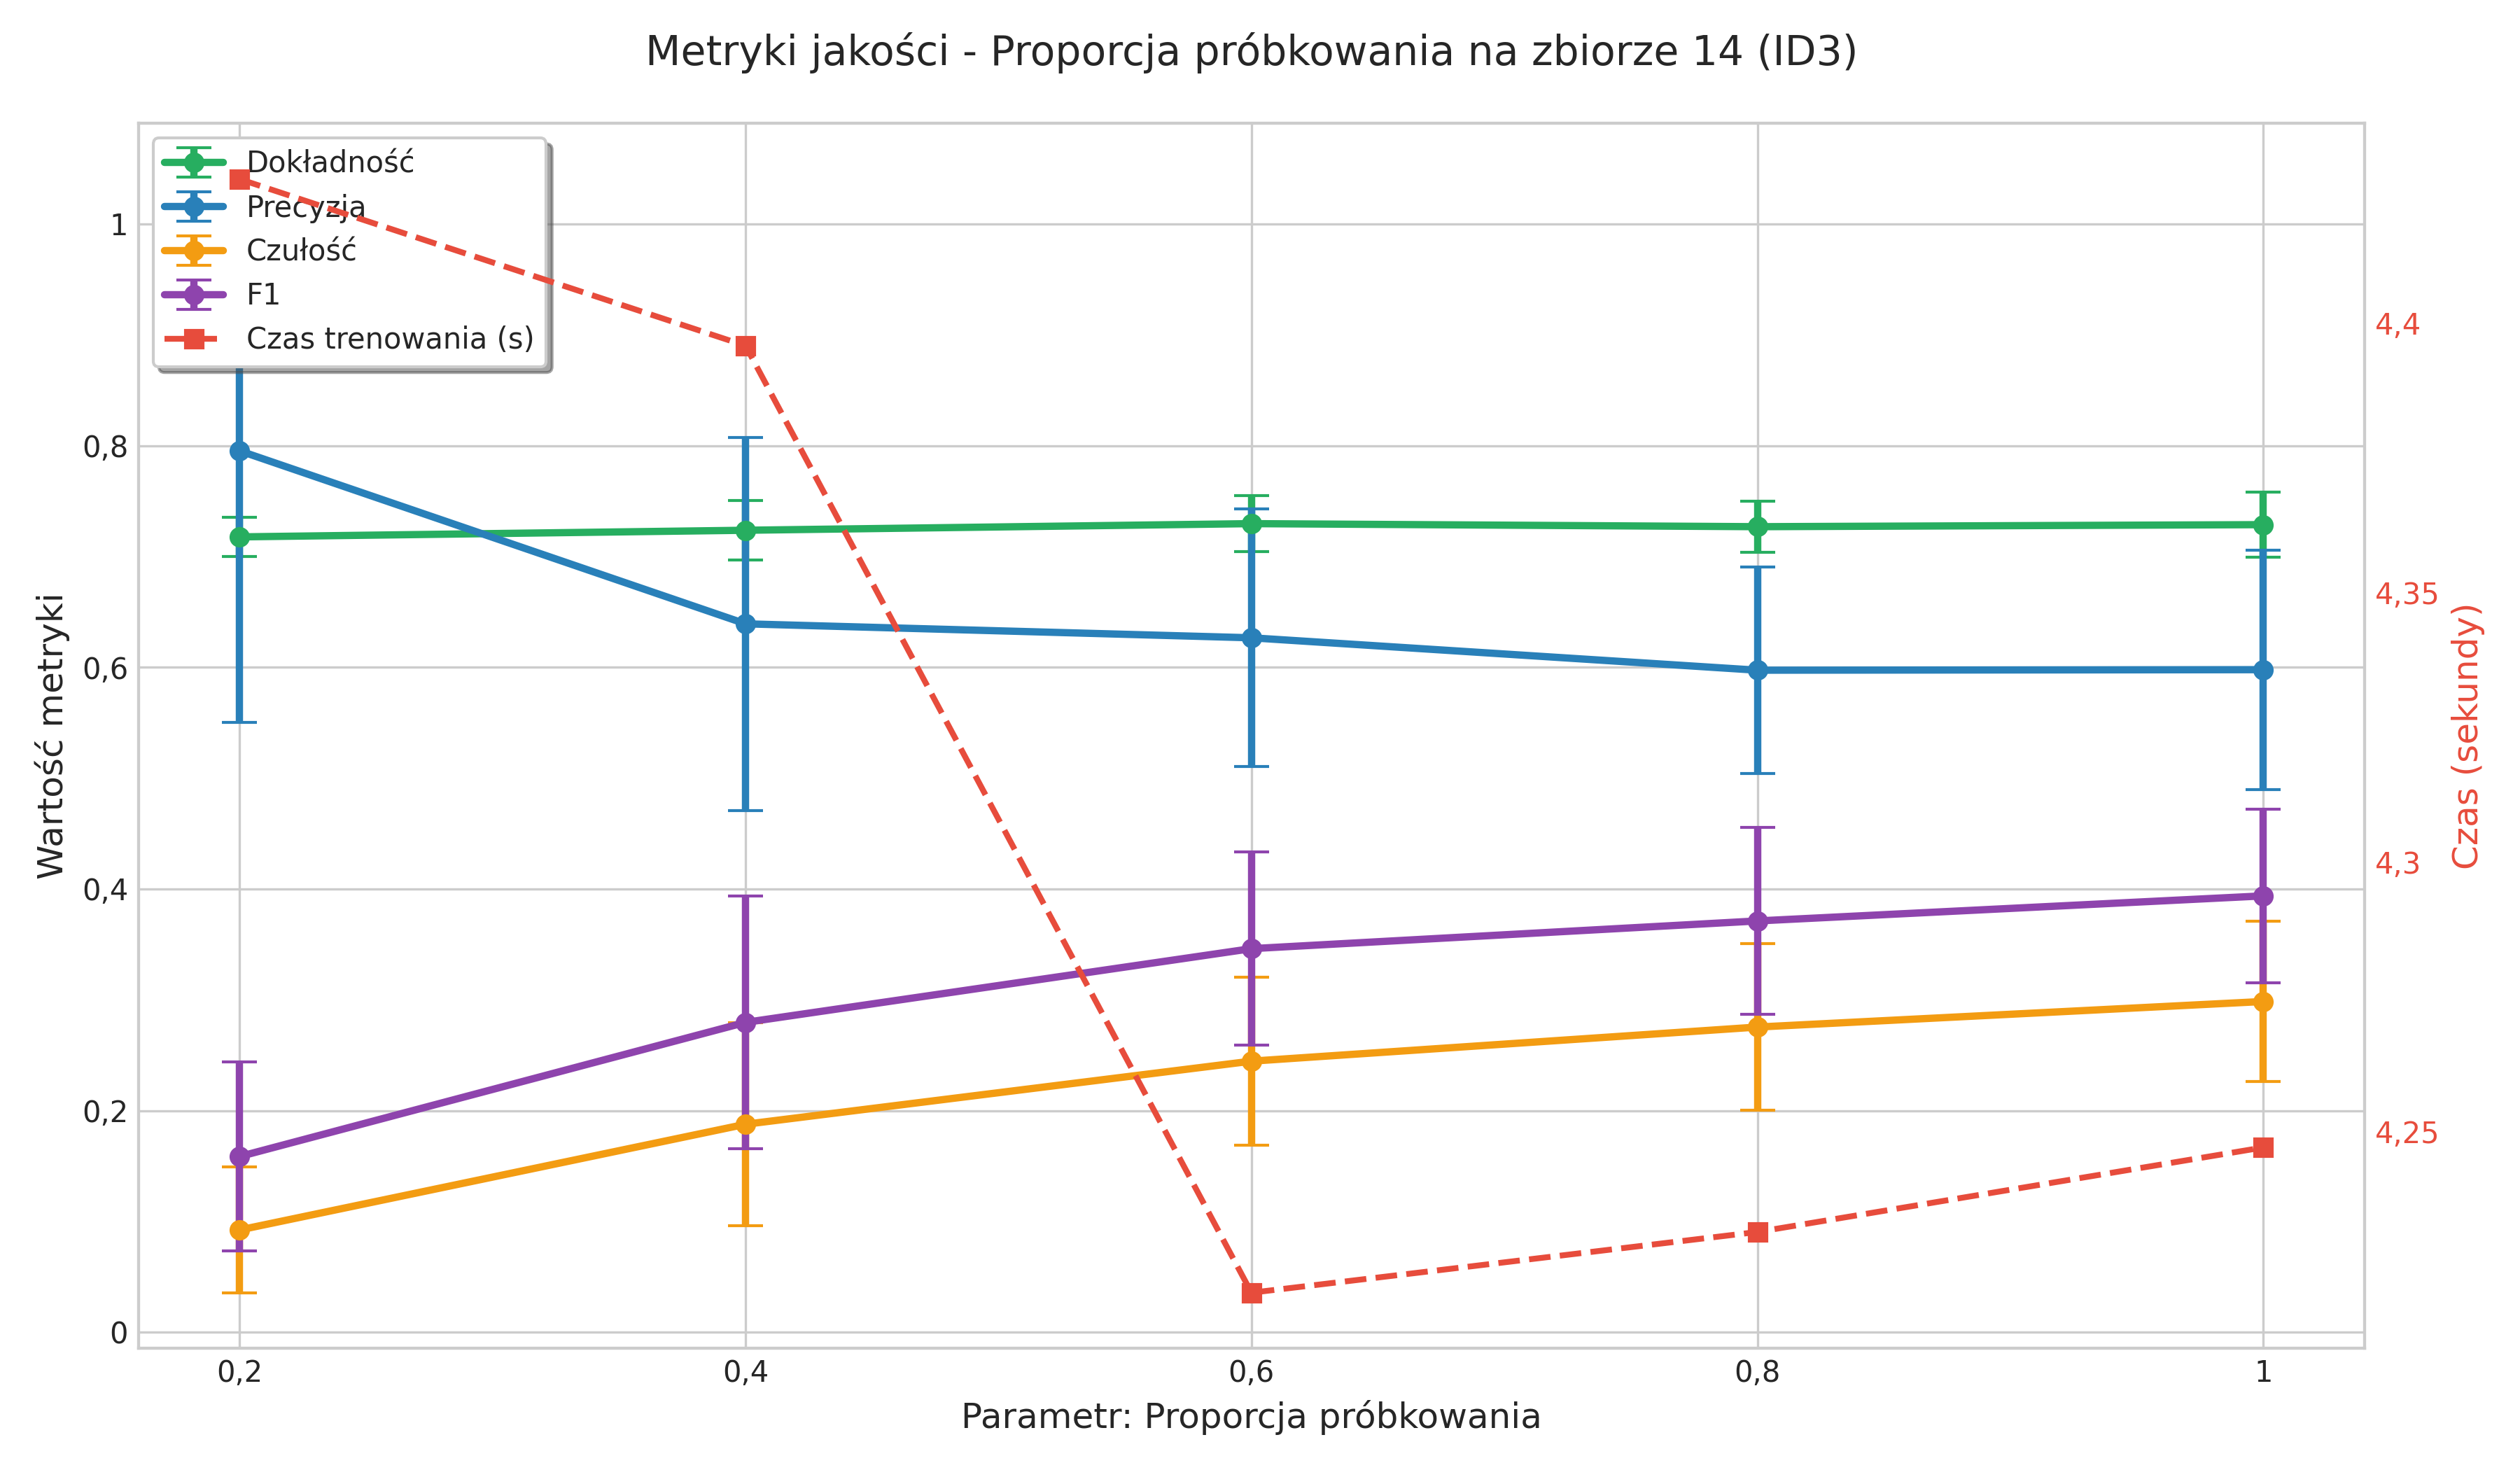
\includegraphics[width=0.9\textwidth]{plots/ID3_sample_ratio_14_metrics.png}
        \caption{Wpływ współczynnika próbkowania na dokładność modelu ID3 dla zbioru 14 - Nawrót raka piersi.}
        \label{fig:id3_sample_ratio_14}
    \end{figure}

\end{itemize}
\subsubsection{CART}
\begin{itemize}
    \item Zbiór 73 - Grzyby

    Na trywialnym zbiorze grzybów optymalne okazuje się ustawienie współczynnika próbkowania w okolicy 70\%. Spadek dokładności przy wartości 100\%
    wskazuje na wystąpienie zjawiska przeuczania w pojedynczych drzewach, które skumulowane wpływa na pogorszenie wyników lasu.

    \begin{figure}[H]
        \centering
        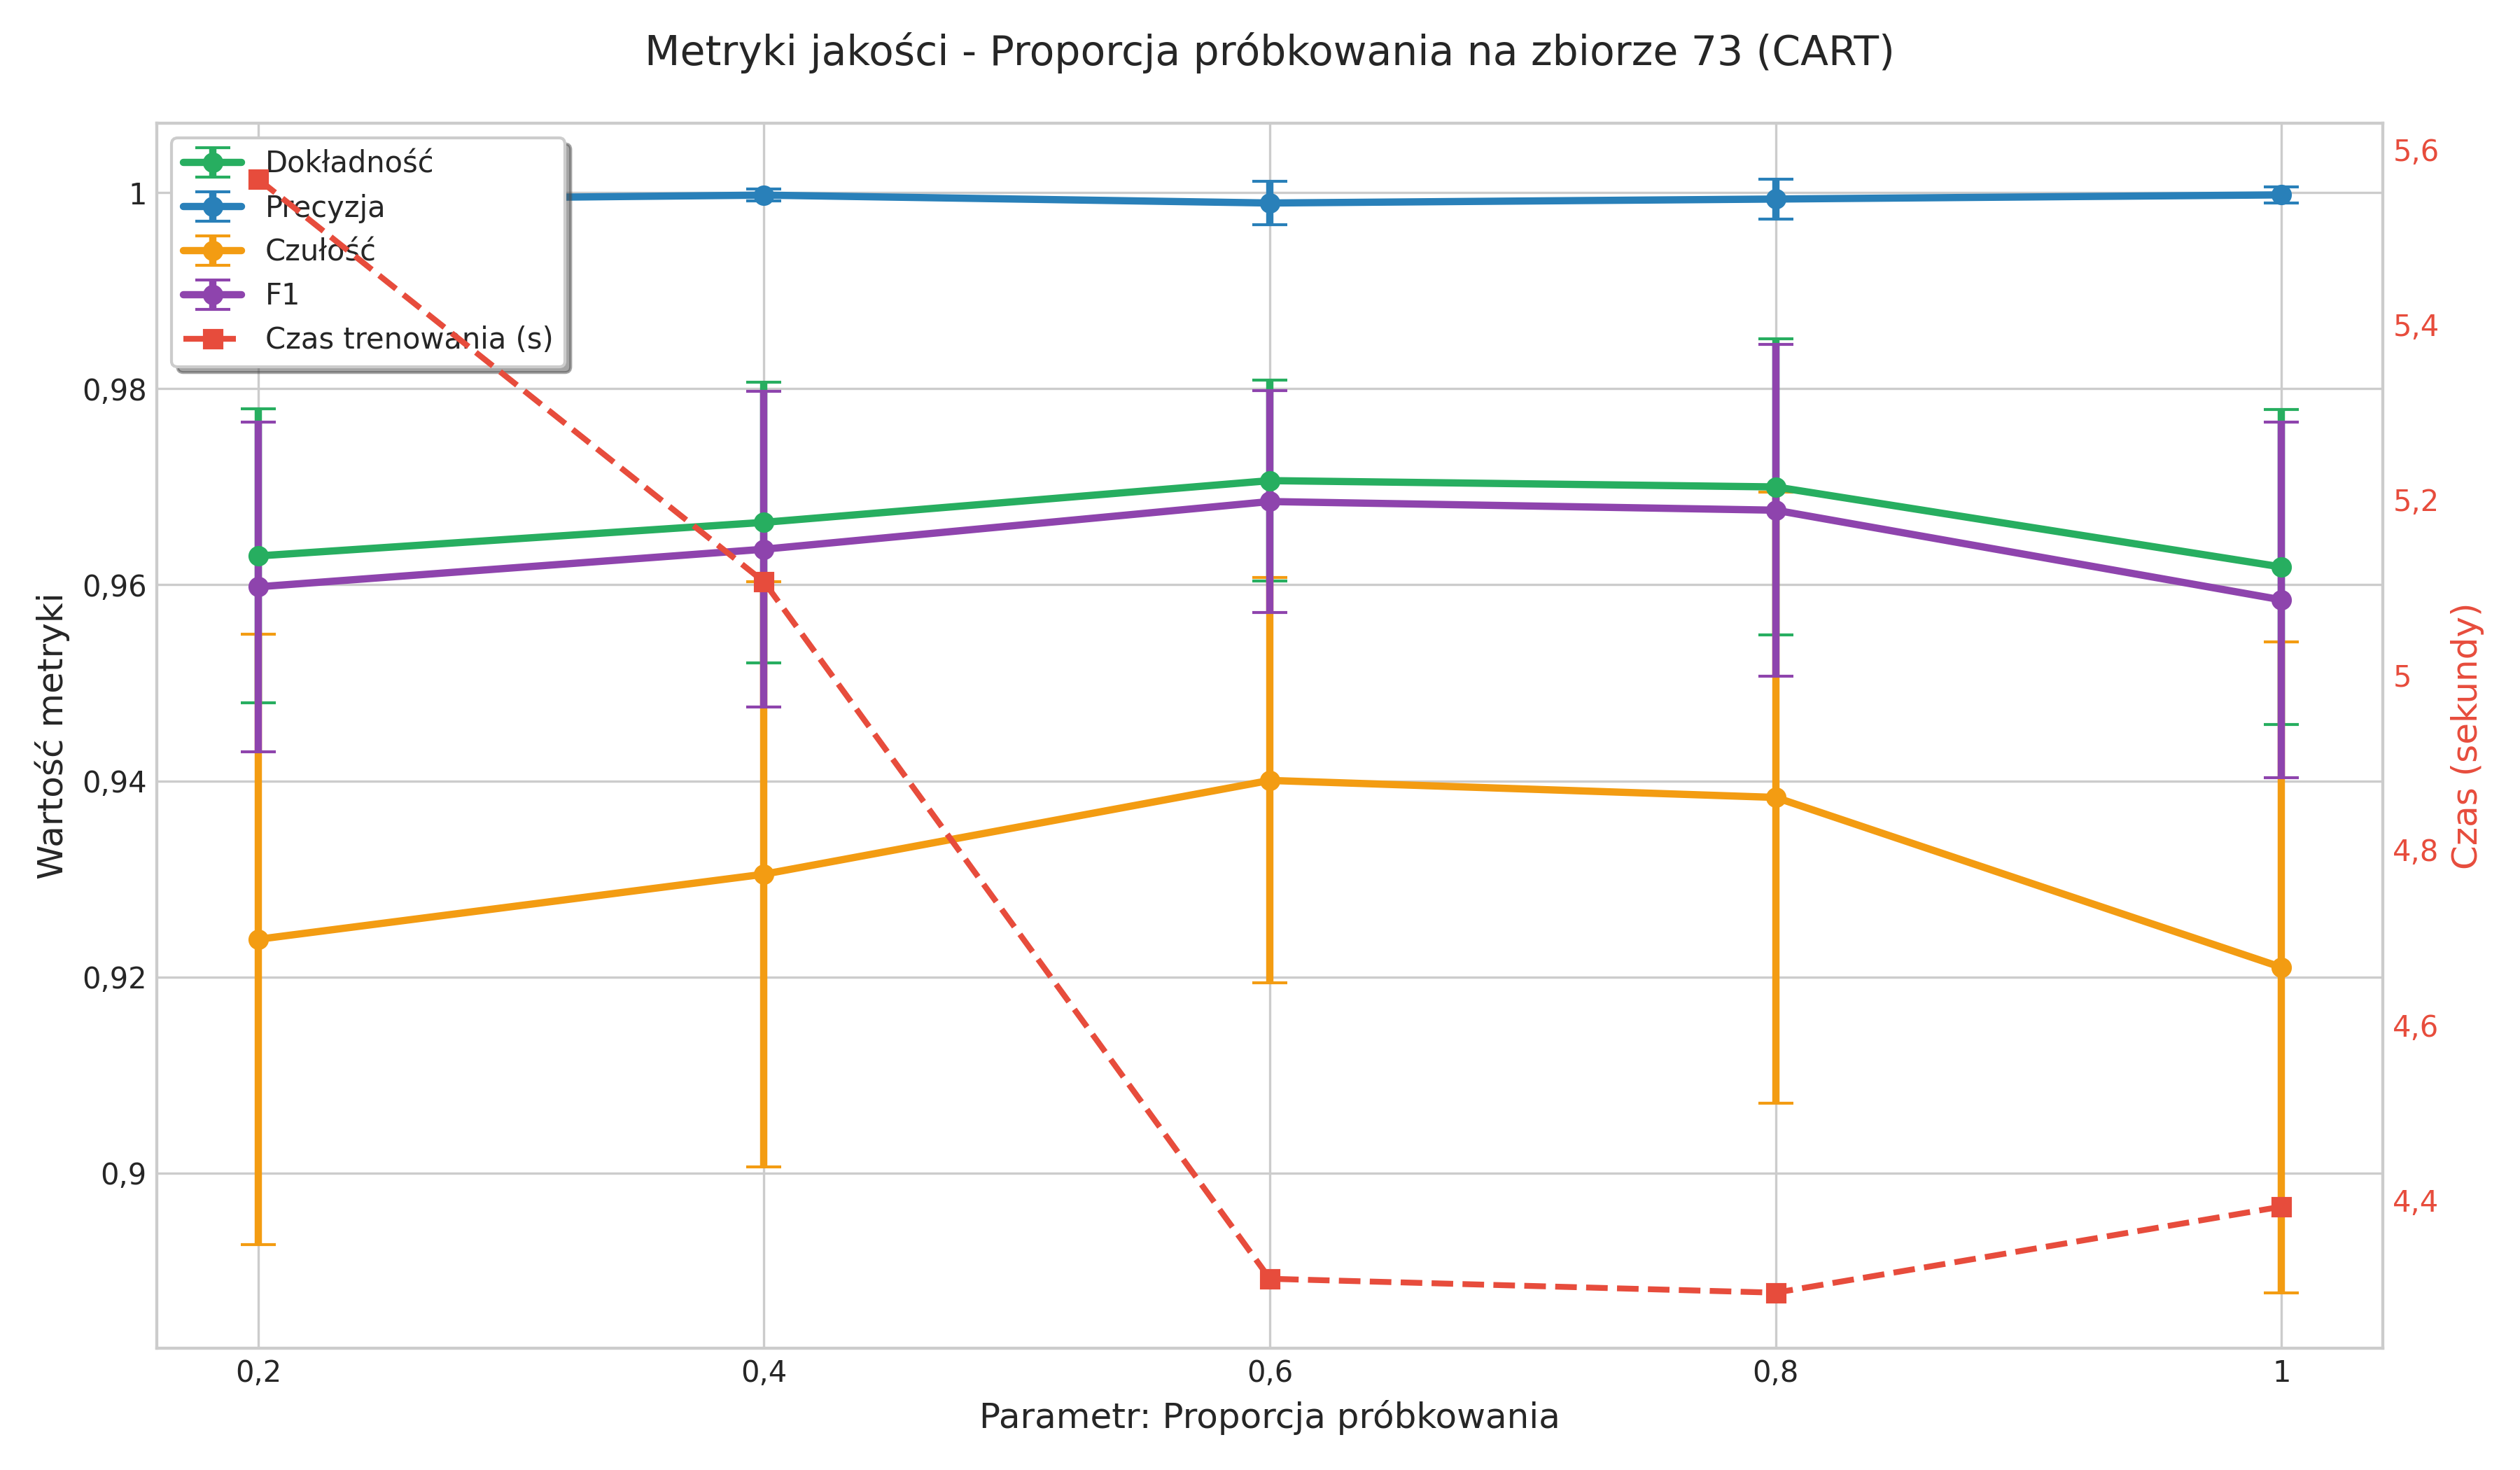
\includegraphics[width=0.9\textwidth]{plots/CART_sample_ratio_73_metrics.png}
        \caption{Wpływ współczynnika próbkowania na dokładność modelu CART dla zbioru 73 - Grzyby.}
        \label{fig:cart_sample_ratio_73}
    \end{figure}

    \item Zbiór 14 - Nawrót raka piersi

    Zbiór ten w przeciwieństwie do grzybów jest trudniejszy, przez co większy współczynnik próbkowania przekłada się na lepsze wyniki.
    100\% okazuje się optymalną wartością, gdyż dla mniejszych wartości obserwujemy niedouczenie drzew.

    \begin{figure}[H]
        \centering
        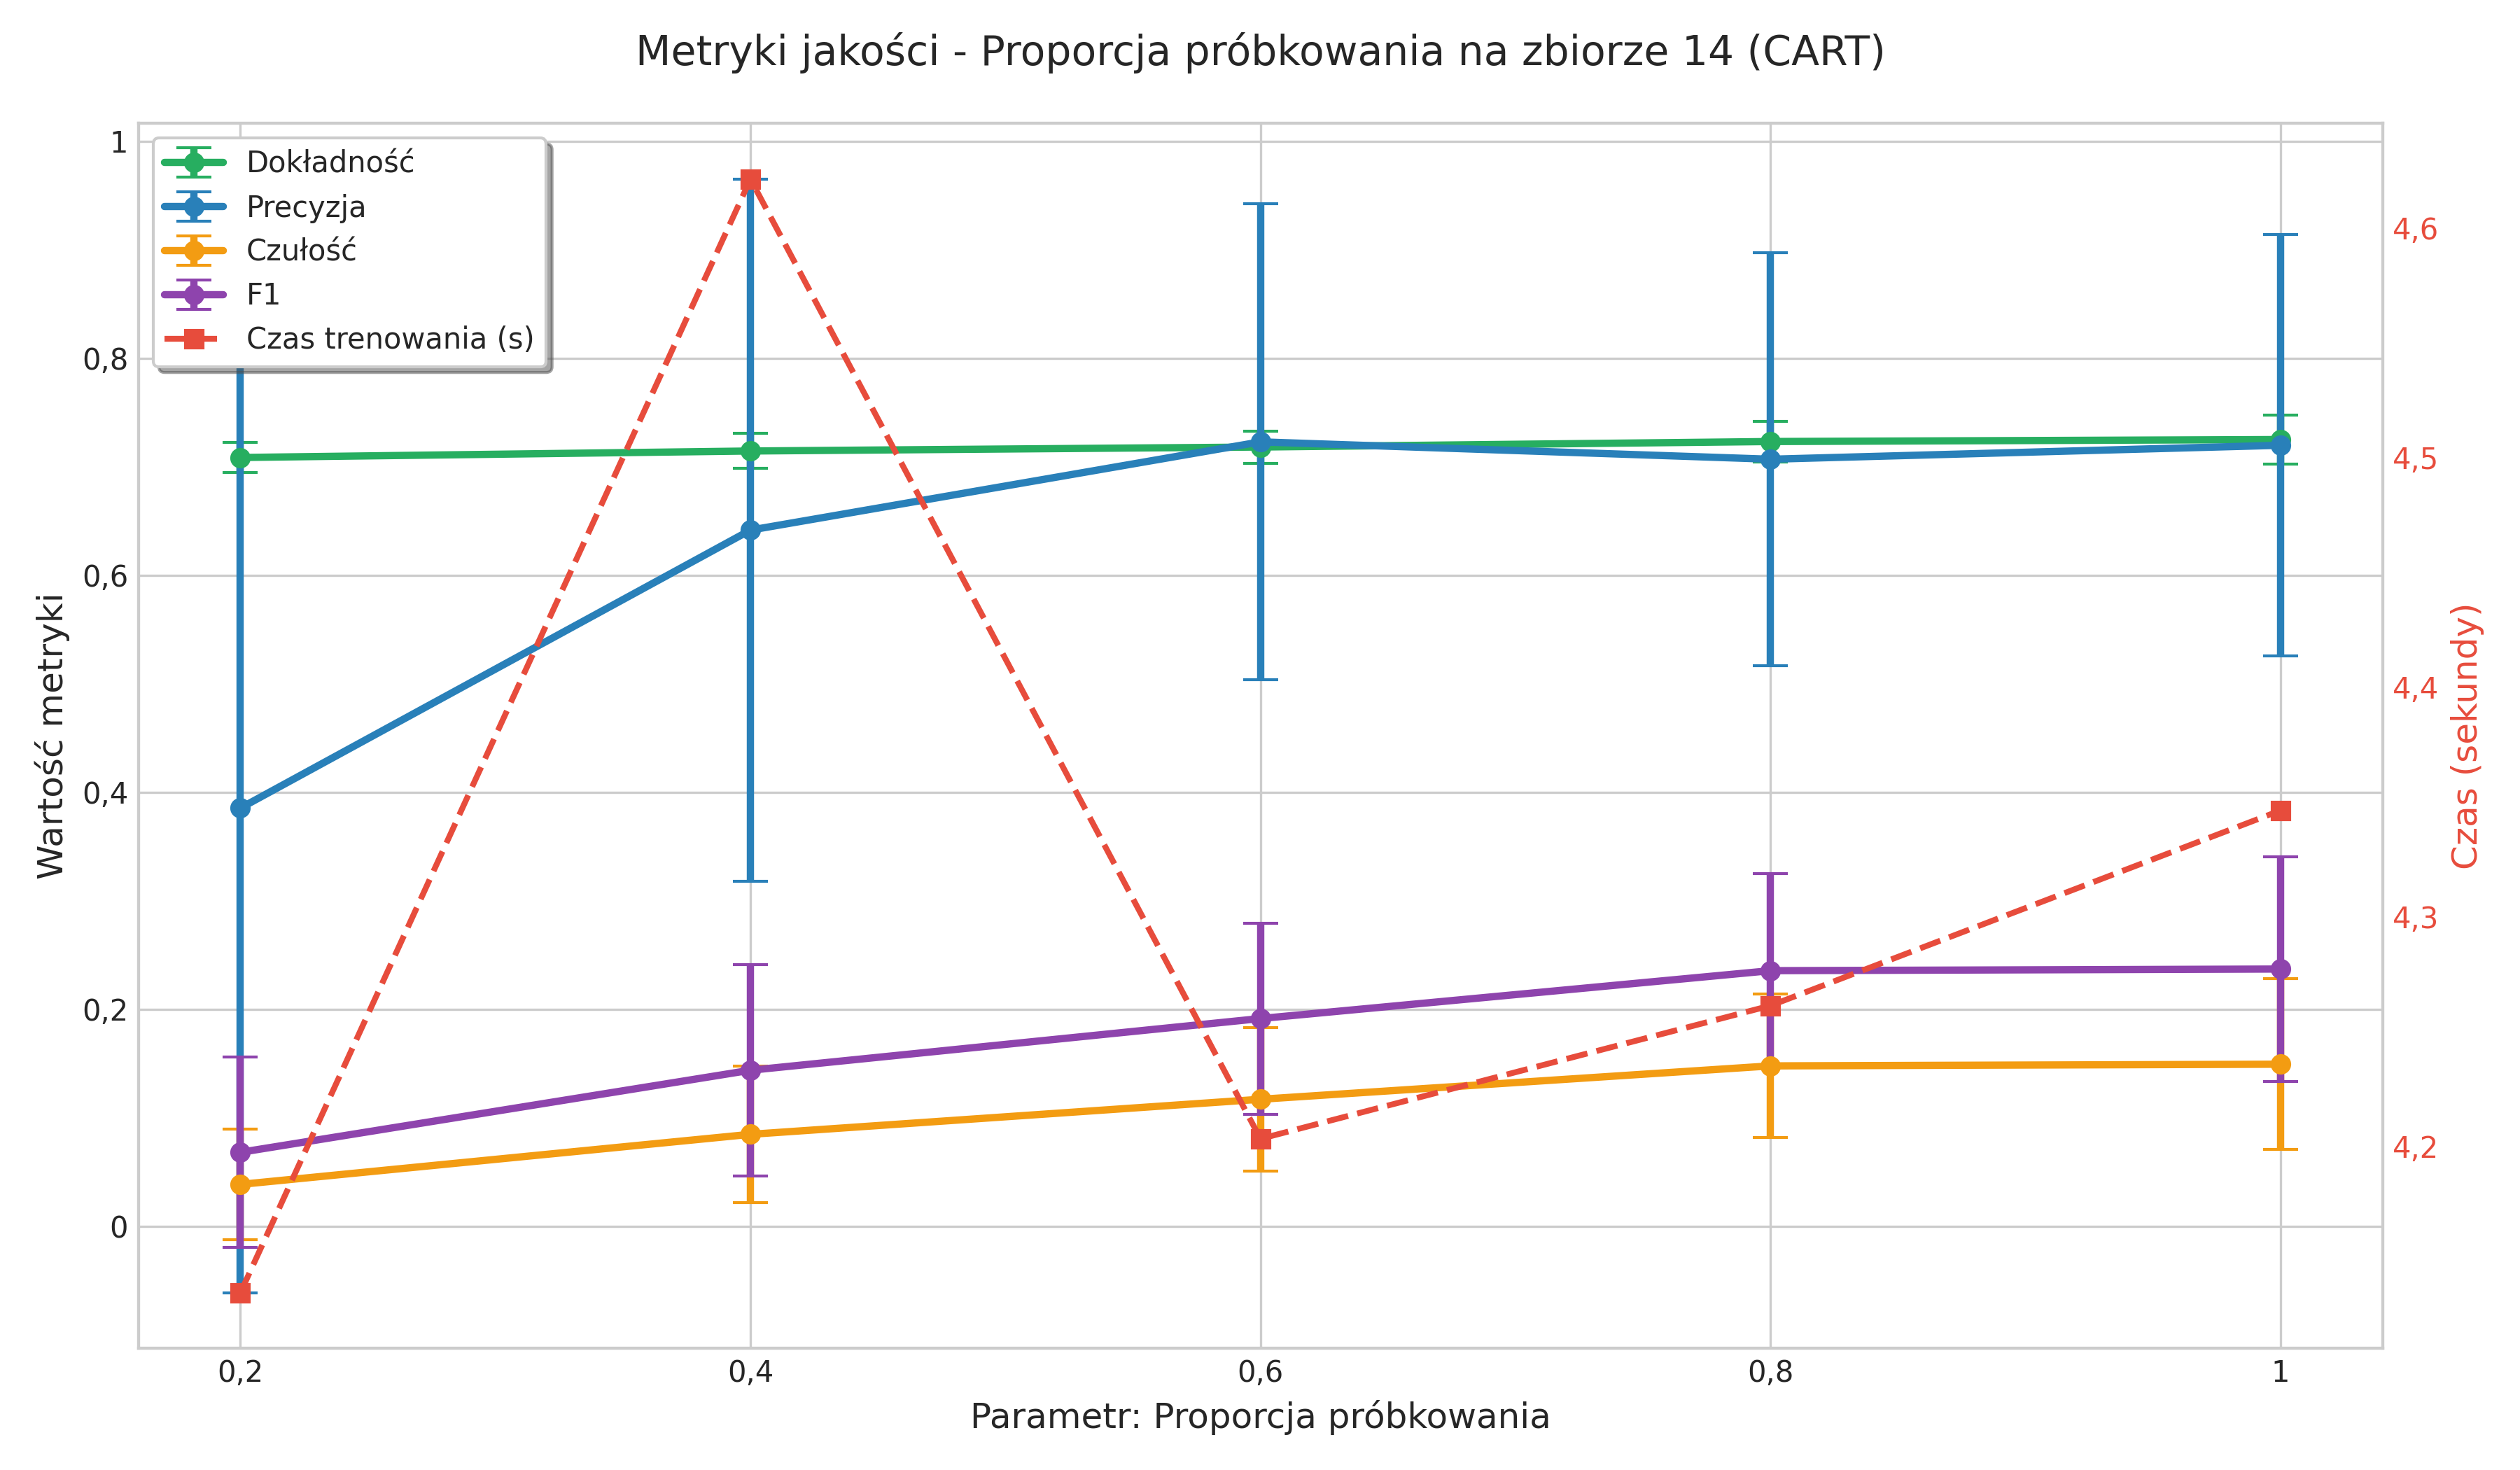
\includegraphics[width=0.9\textwidth]{plots/CART_sample_ratio_14_metrics.png}
        \caption{Wpływ współczynnika próbkowania na dokładność modelu CART dla zbioru 14 - Nawrót raka piersi.}
        \label{fig:cart_sample_ratio_14}
    \end{figure}

    \item Zbiór 222 - Skuteczność marketingu bankowego

    Na dużych zbiorach z niezbalansowanymi klasami sterowanie współczynnikiem próbkowania nie wpływa znacząco na uzyskiwane wyniki.

    \begin{figure}[H]
        \centering
        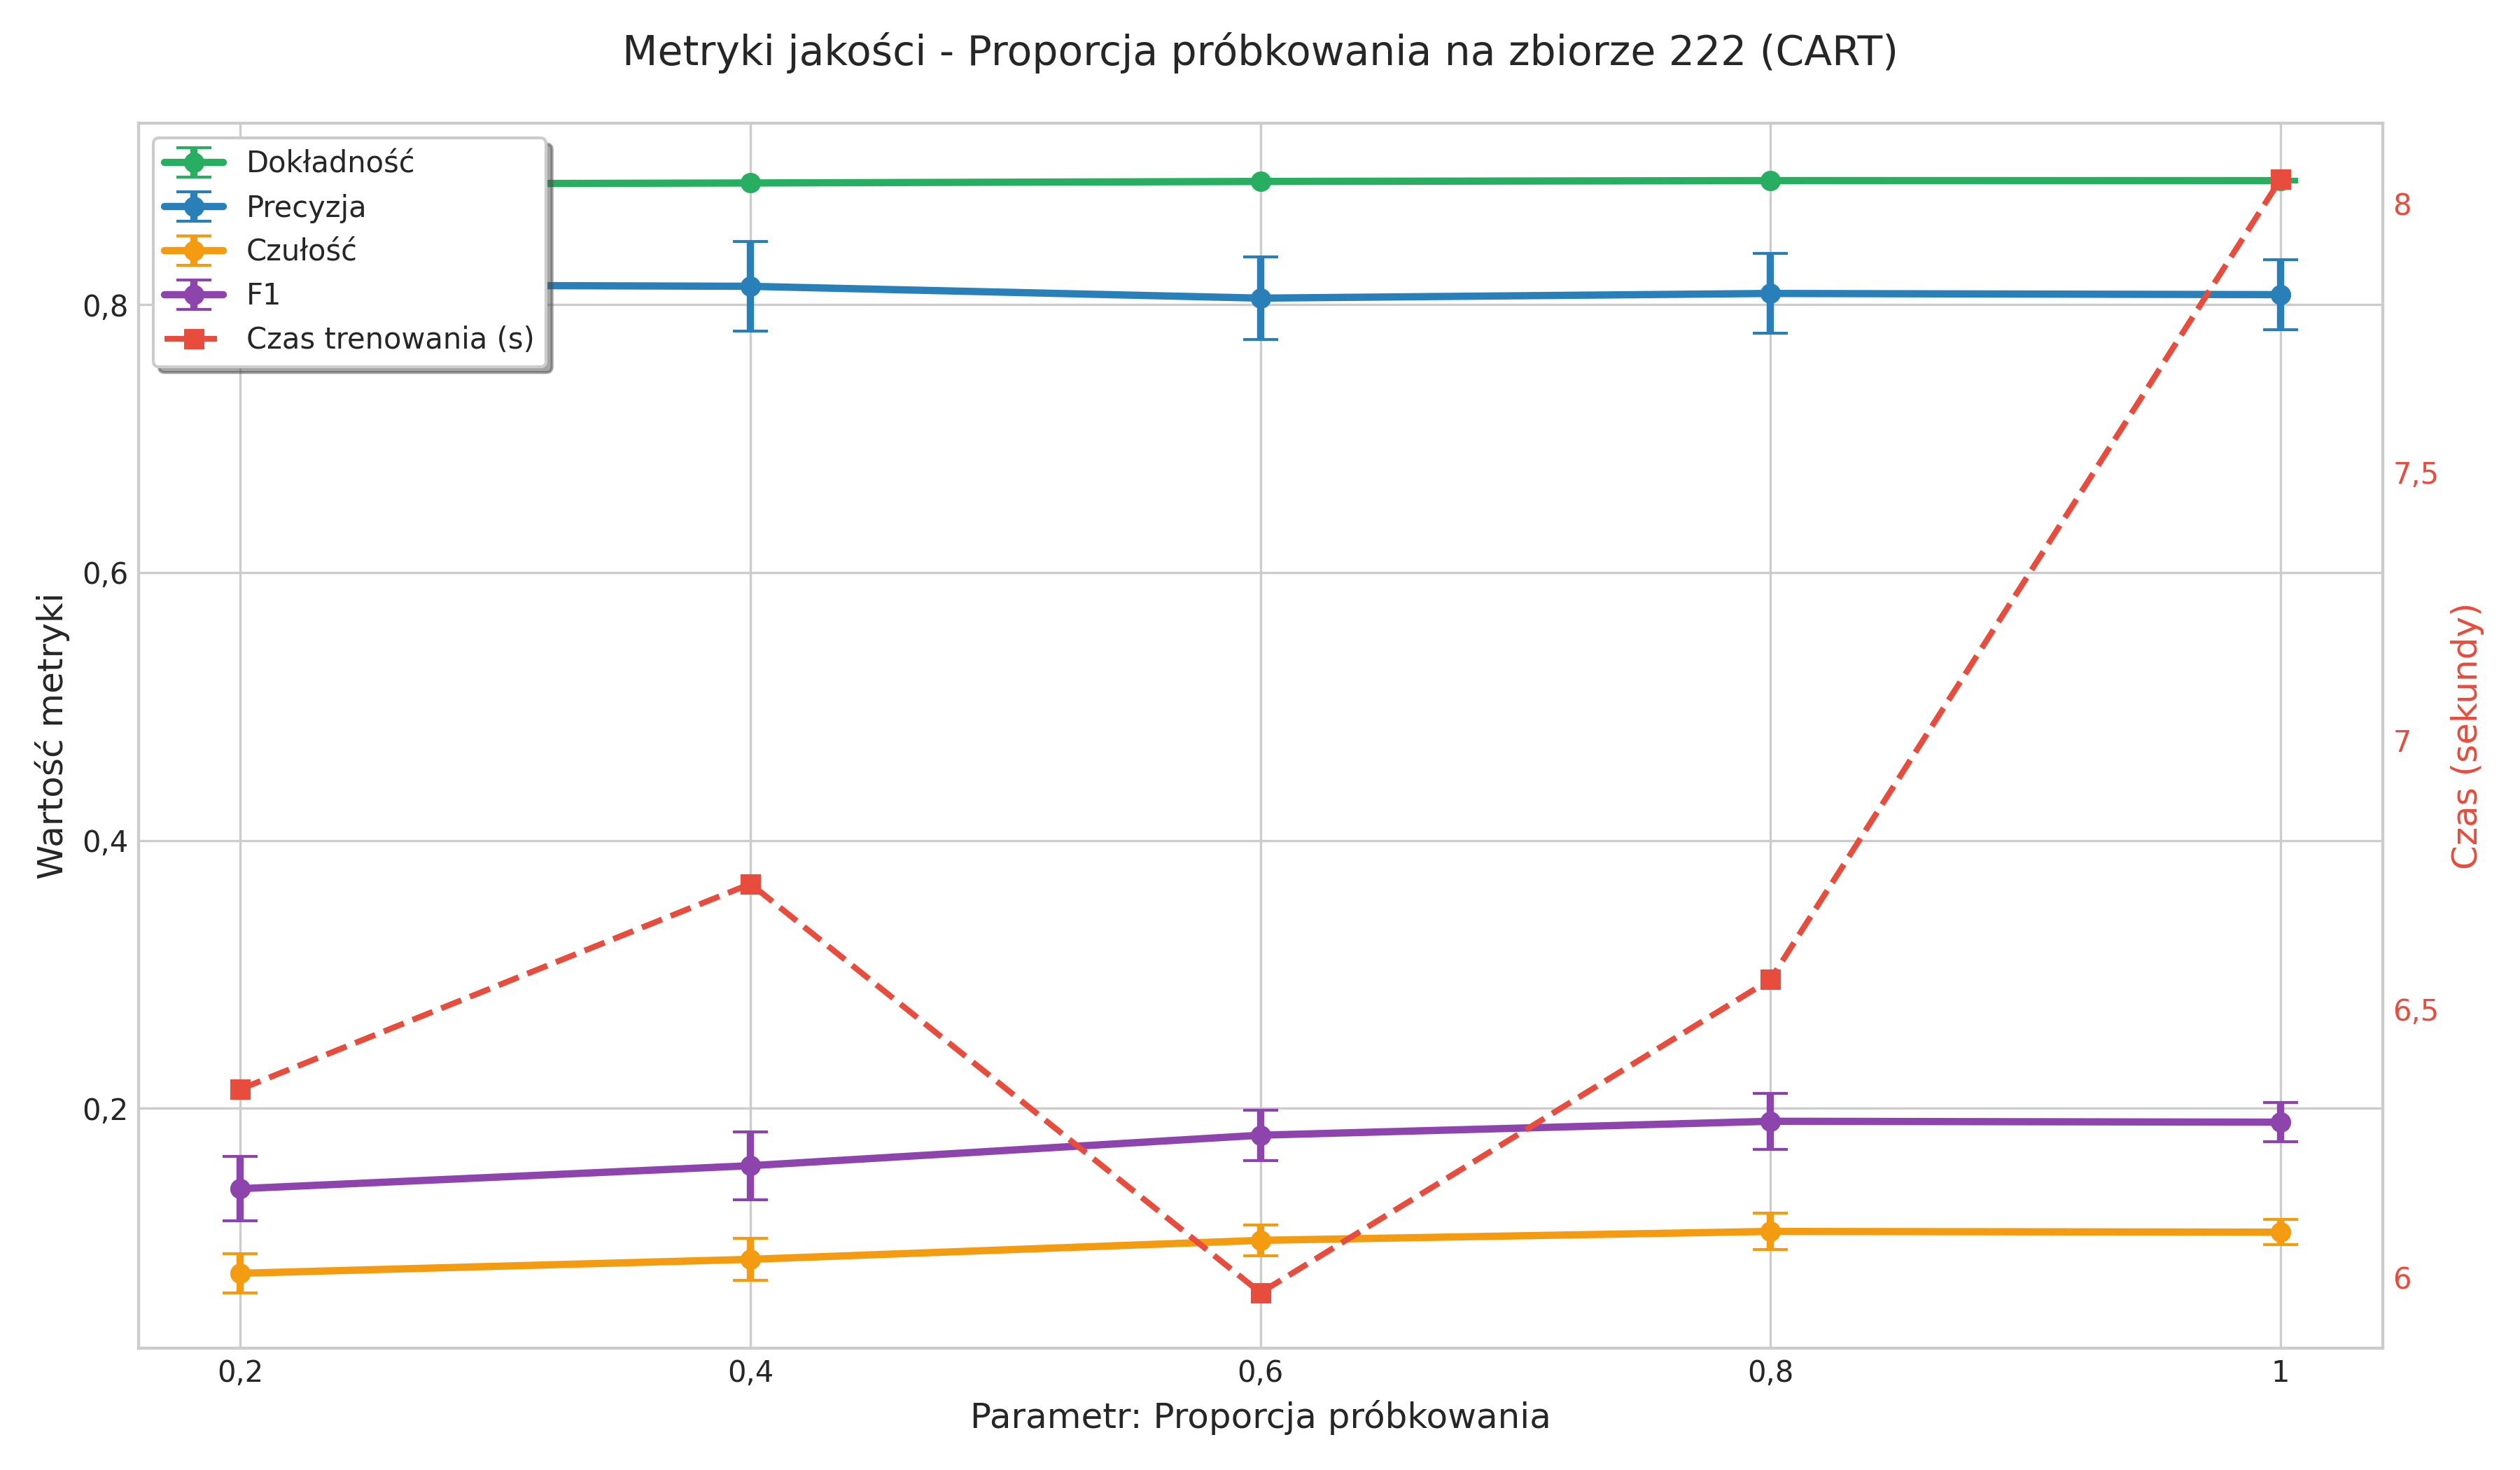
\includegraphics[width=0.9\textwidth]{plots/CART_sample_ratio_222_metrics.png}
        \caption{Wpływ współczynnika próbkowania na dokładność modelu CART dla zbioru 222 - Skuteczność marketingu bankowego.}
        \label{fig:cart_sample_ratio_222}
    \end{figure}

    \item Zbiór 350 - Zaległości płatnicze klientów kart kredytowych

    Na dużych zbiorach z niezbalansowanymi klasami sterowanie współczynnikiem próbkowania nie wpływa znacząco na uzyskiwane wyniki.

    \begin{figure}[H]
        \centering
        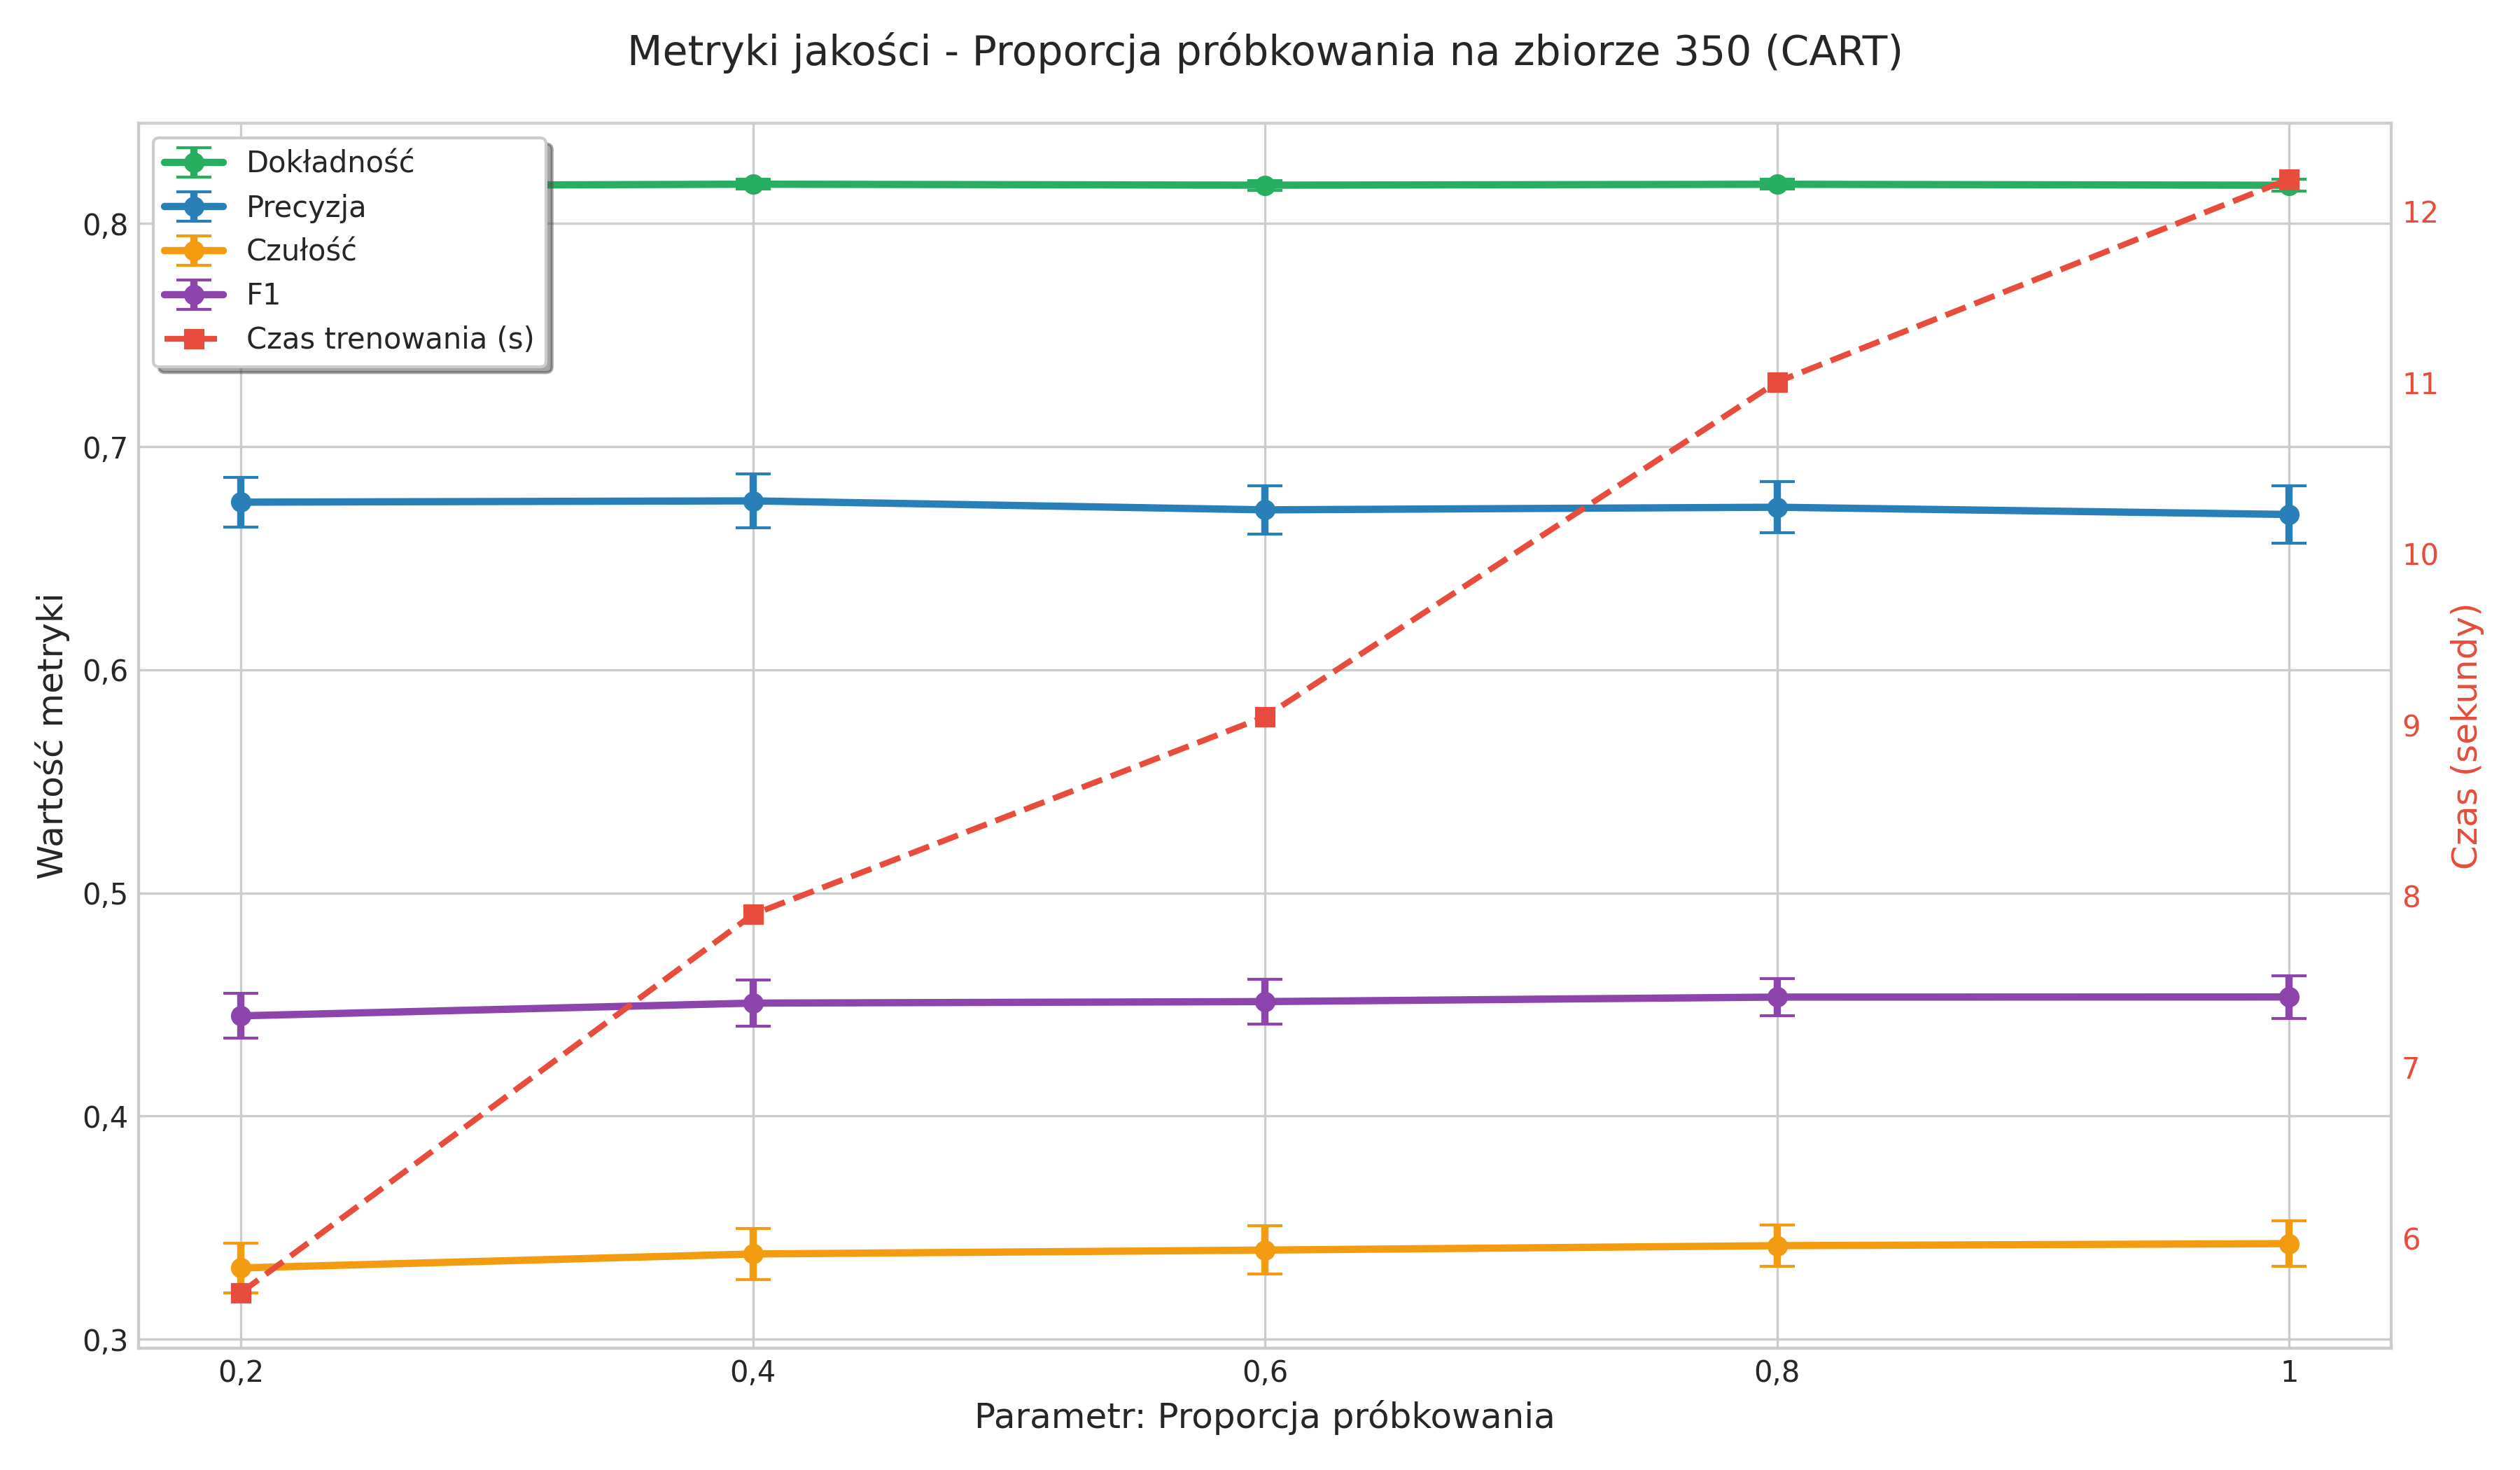
\includegraphics[width=0.9\textwidth]{plots/CART_sample_ratio_350_metrics.png}
        \caption{Wpływ współczynnika próbkowania na dokładność modelu CART dla zbioru 350 - Zaległości płatnicze klientów kart kredytowych.}
        \label{fig:cart_sample_ratio_350}
    \end{figure}
\end{itemize}

\subsubsection{Wnioski ogólne}
\begin{itemize}
    \item Stosowanie współczynnika próbkowania poniżej 100\% jest uzasadnione jedynie w przypadku, gdy zbiór danych jest mały oraz nietrywialny.
    Wtedy przyjęcie wartości w okolicy 70\% pozwala na redukcję zjawiska przeuczania.
    \item W pozostałych przypadkach stosowanie współczynnika próbkowania równego 100\% pozwala na uzyskanie najlepszych wyników.
\end{itemize}


\subsection{Maksymalna głębokość drzew}

\subsubsection{ID3}
\begin{itemize}
    \item Zbiór 73 - Grzyby

    Nawet przy minimalnej głębokości drzewa model osiąga 100\% dokładności, co wskazuje na trywialność zbioru.

    \begin{figure}[H]
        \centering
        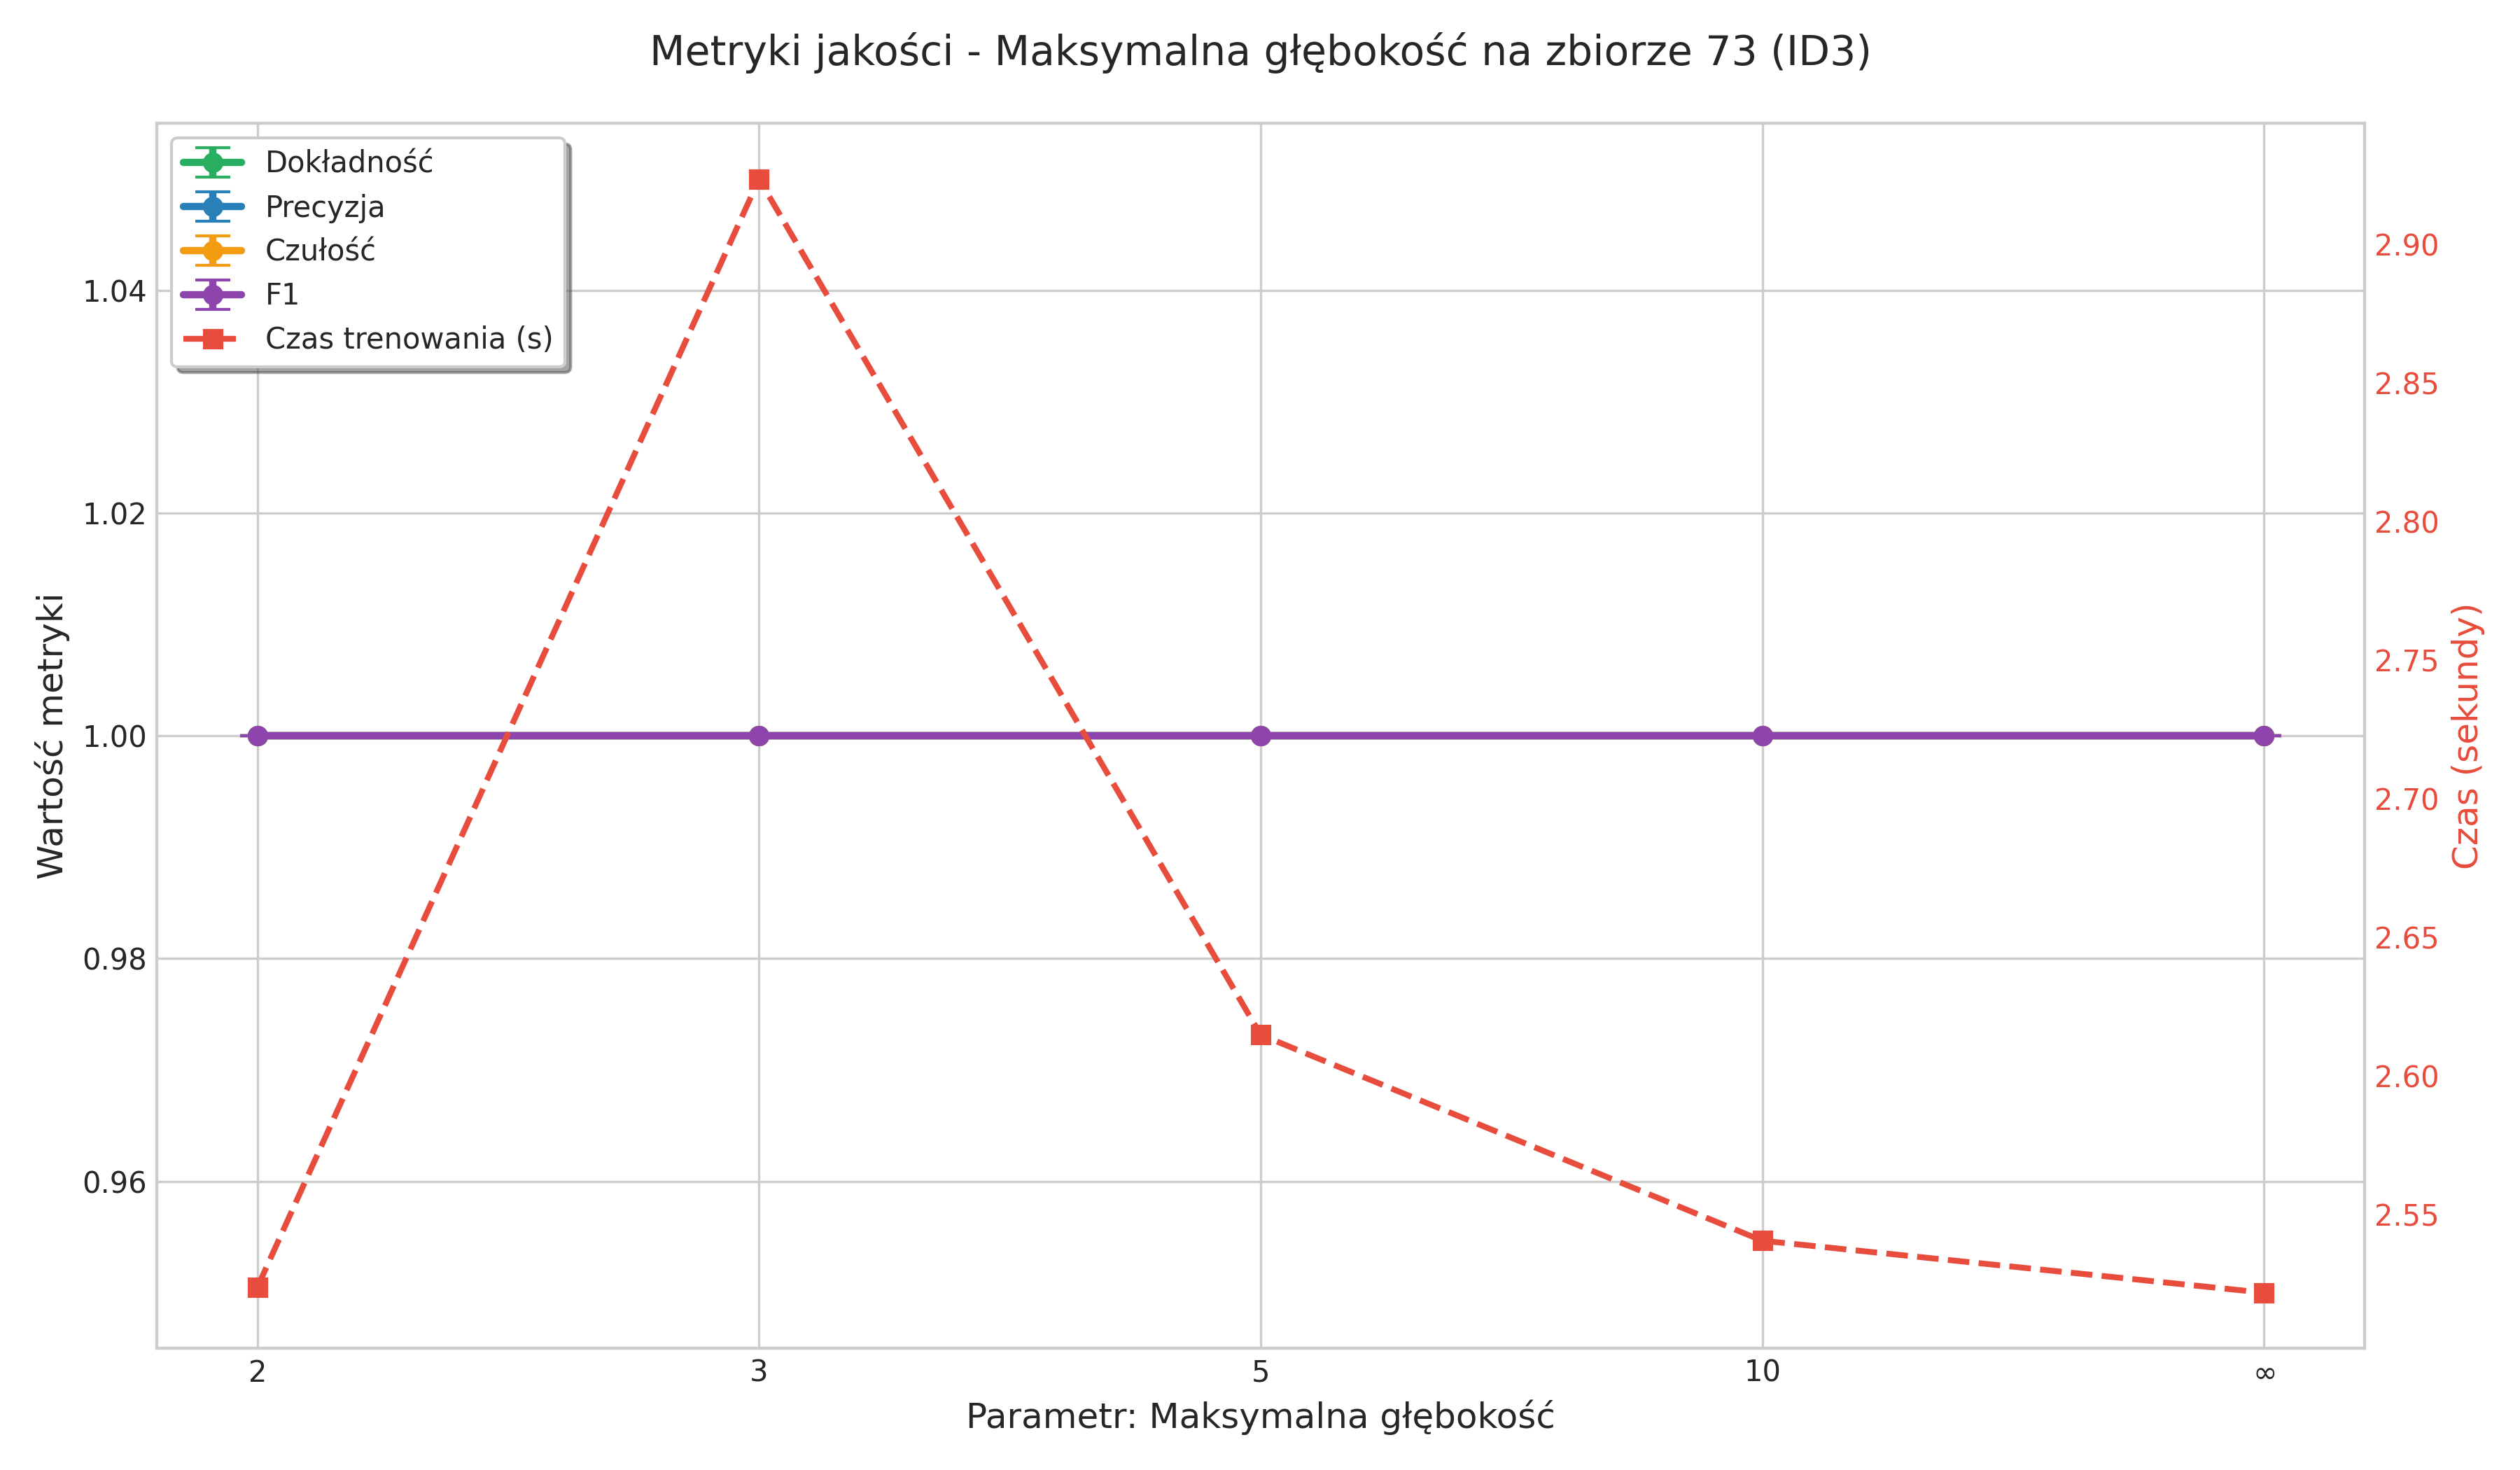
\includegraphics[width=0.9\textwidth]{plots/ID3_max_depth_73_metrics.png}
        \caption{Wpływ maksymalnej głębokości na dokładność modelu ID3 dla zbioru 73 - Grzyby.}
        \label{fig:id3_max_depth_73}
    \end{figure}

    \item Zbiór 14 - Nawrót raka piersi

    Maksymalna głębokość drzewa nie wpływa na wyniki modelu.

    \begin{figure}[H]
        \centering
        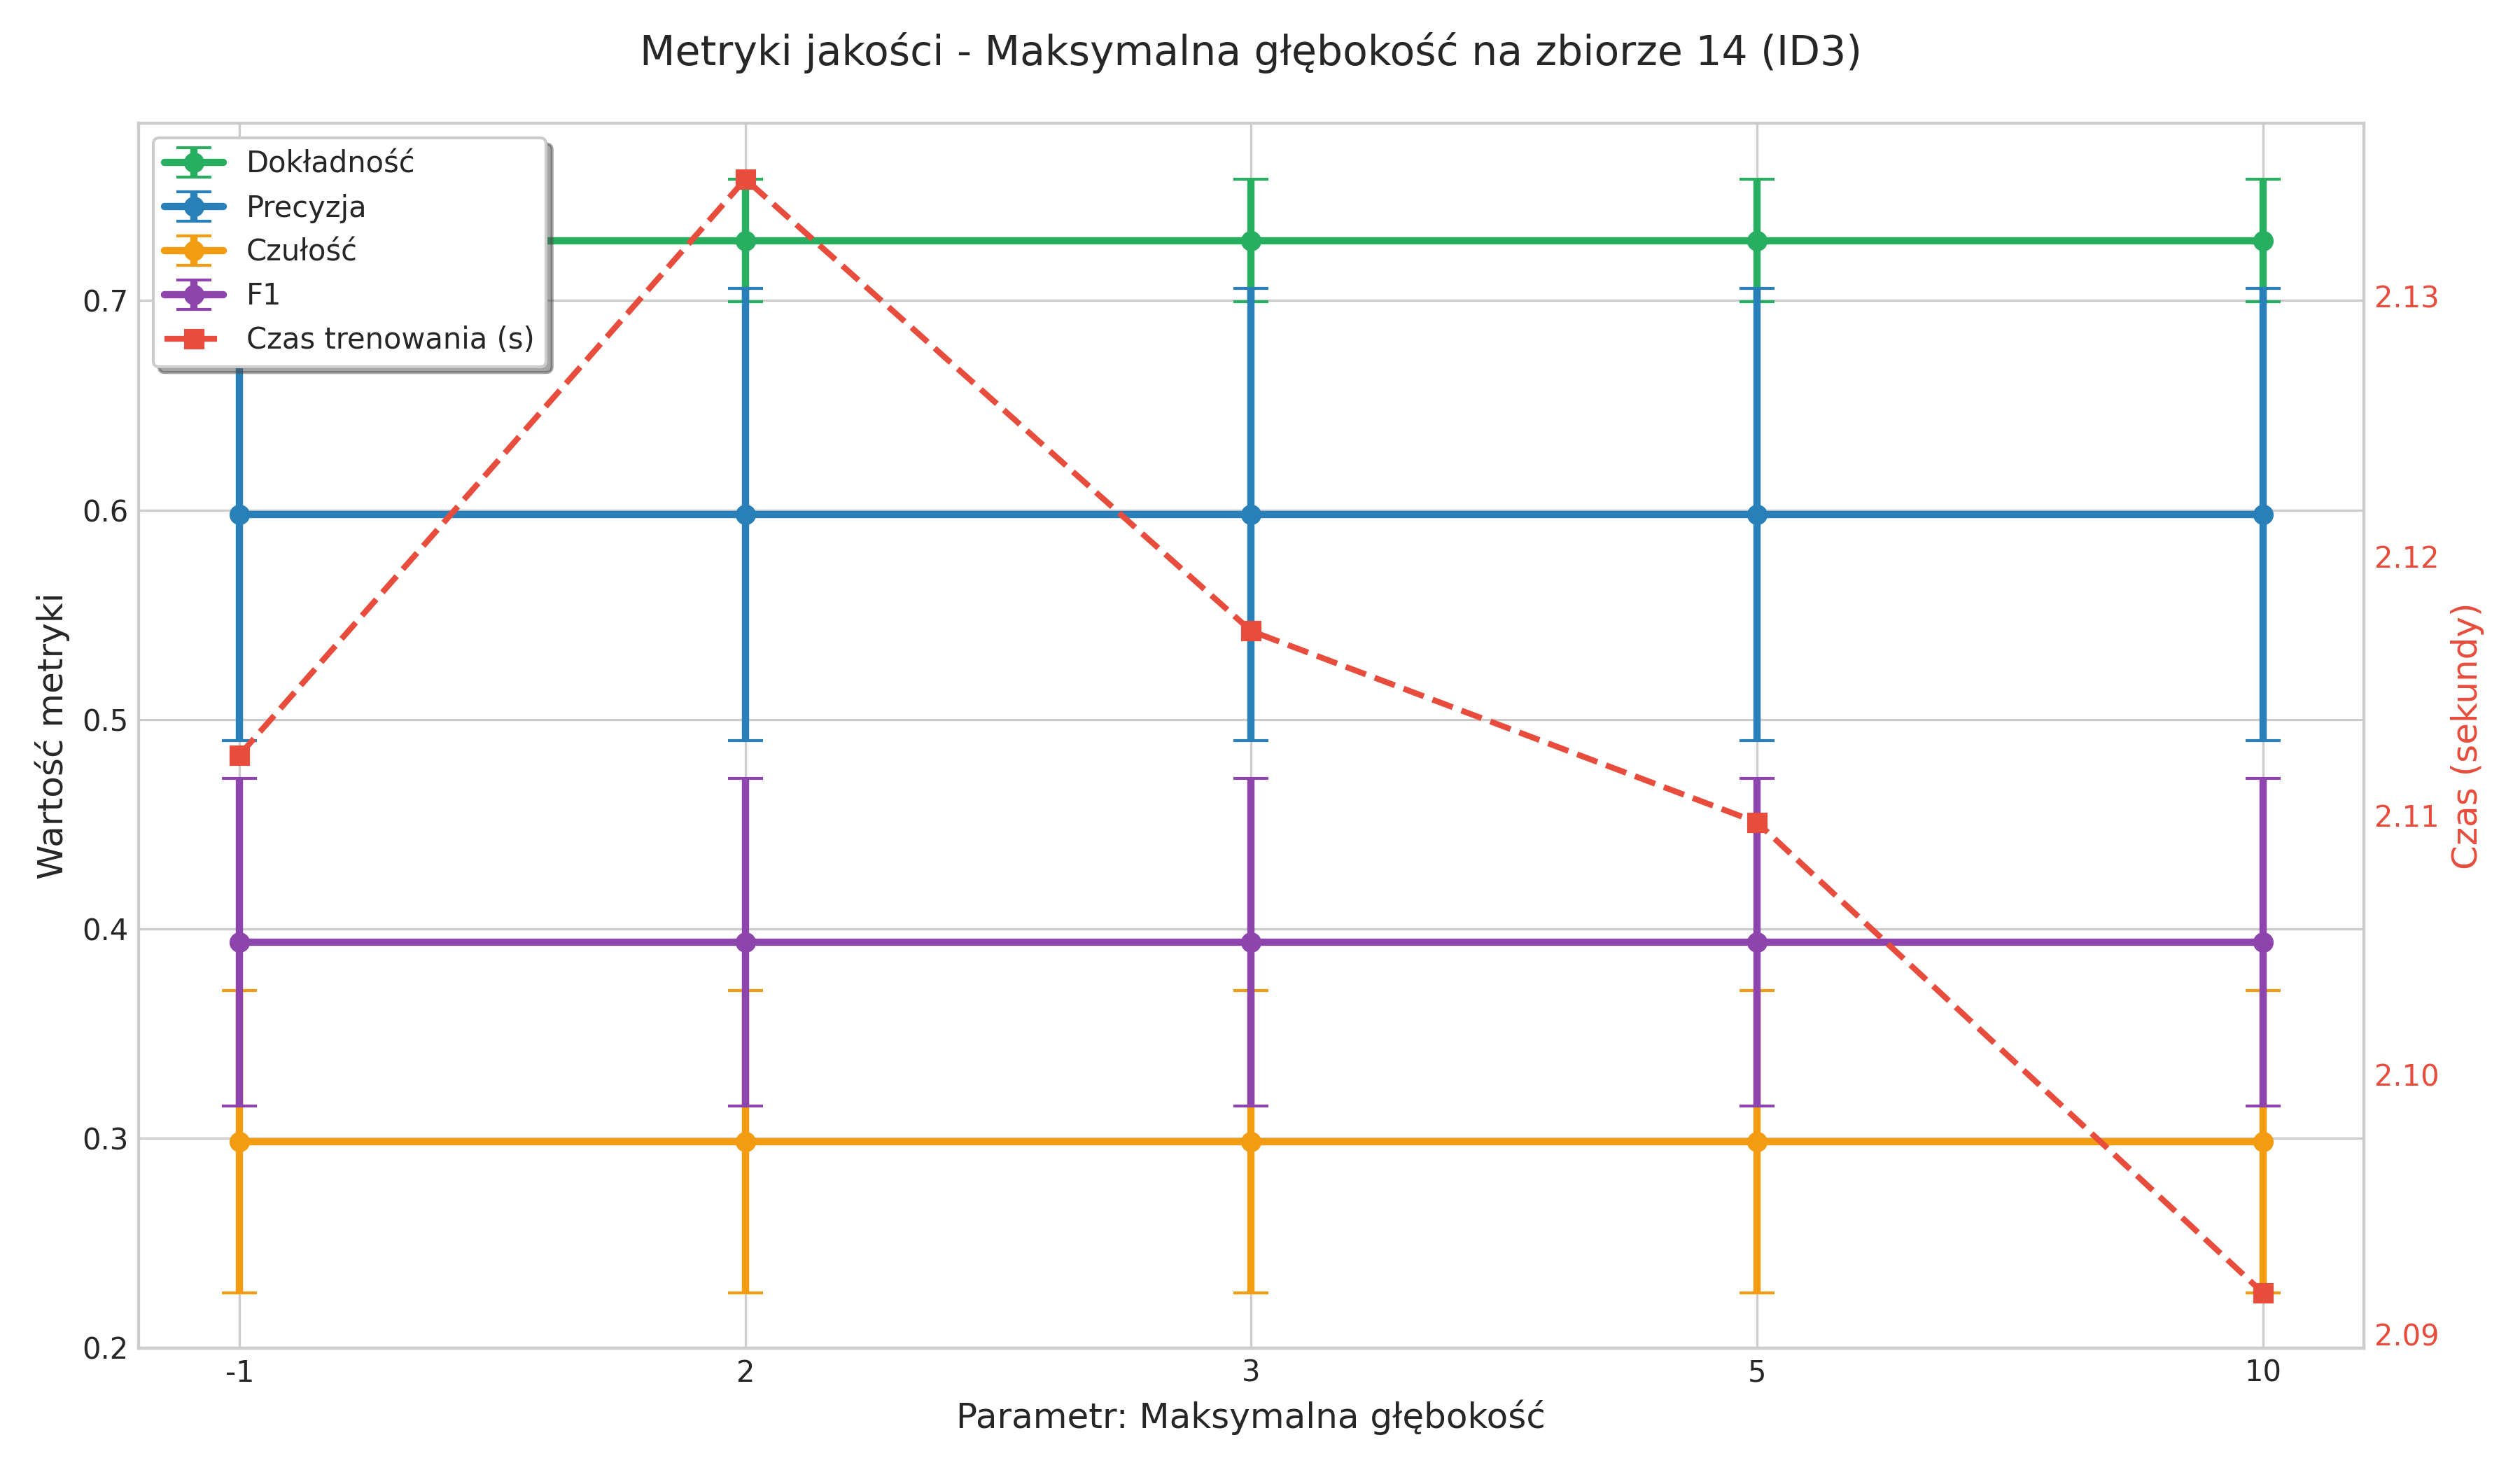
\includegraphics[width=0.9\textwidth]{plots/ID3_max_depth_14_metrics.png}
        \caption{Wpływ maksymalnej głębokości na dokładność modelu ID3 dla zbioru 14 - Nawrót raka piersi.}
        \label{fig:id3_max_depth_14}
    \end{figure}

\end{itemize}
\subsubsection{CART}
\begin{itemize}
    \item Zbiór 73 - Grzyby

    Obserwujemy poprawę wyników modelu wraz ze wzrostem maksymalnej głębokości drzew. Wynika to z faktu, iż atrybuty kategoryczne
    zostały zakodowane za pomocą one-hot encoding, co zwiększa wymiarowość danych i wymaga głębszych drzew do skutecznej separacji klas.

    \begin{figure}[H]
        \centering
        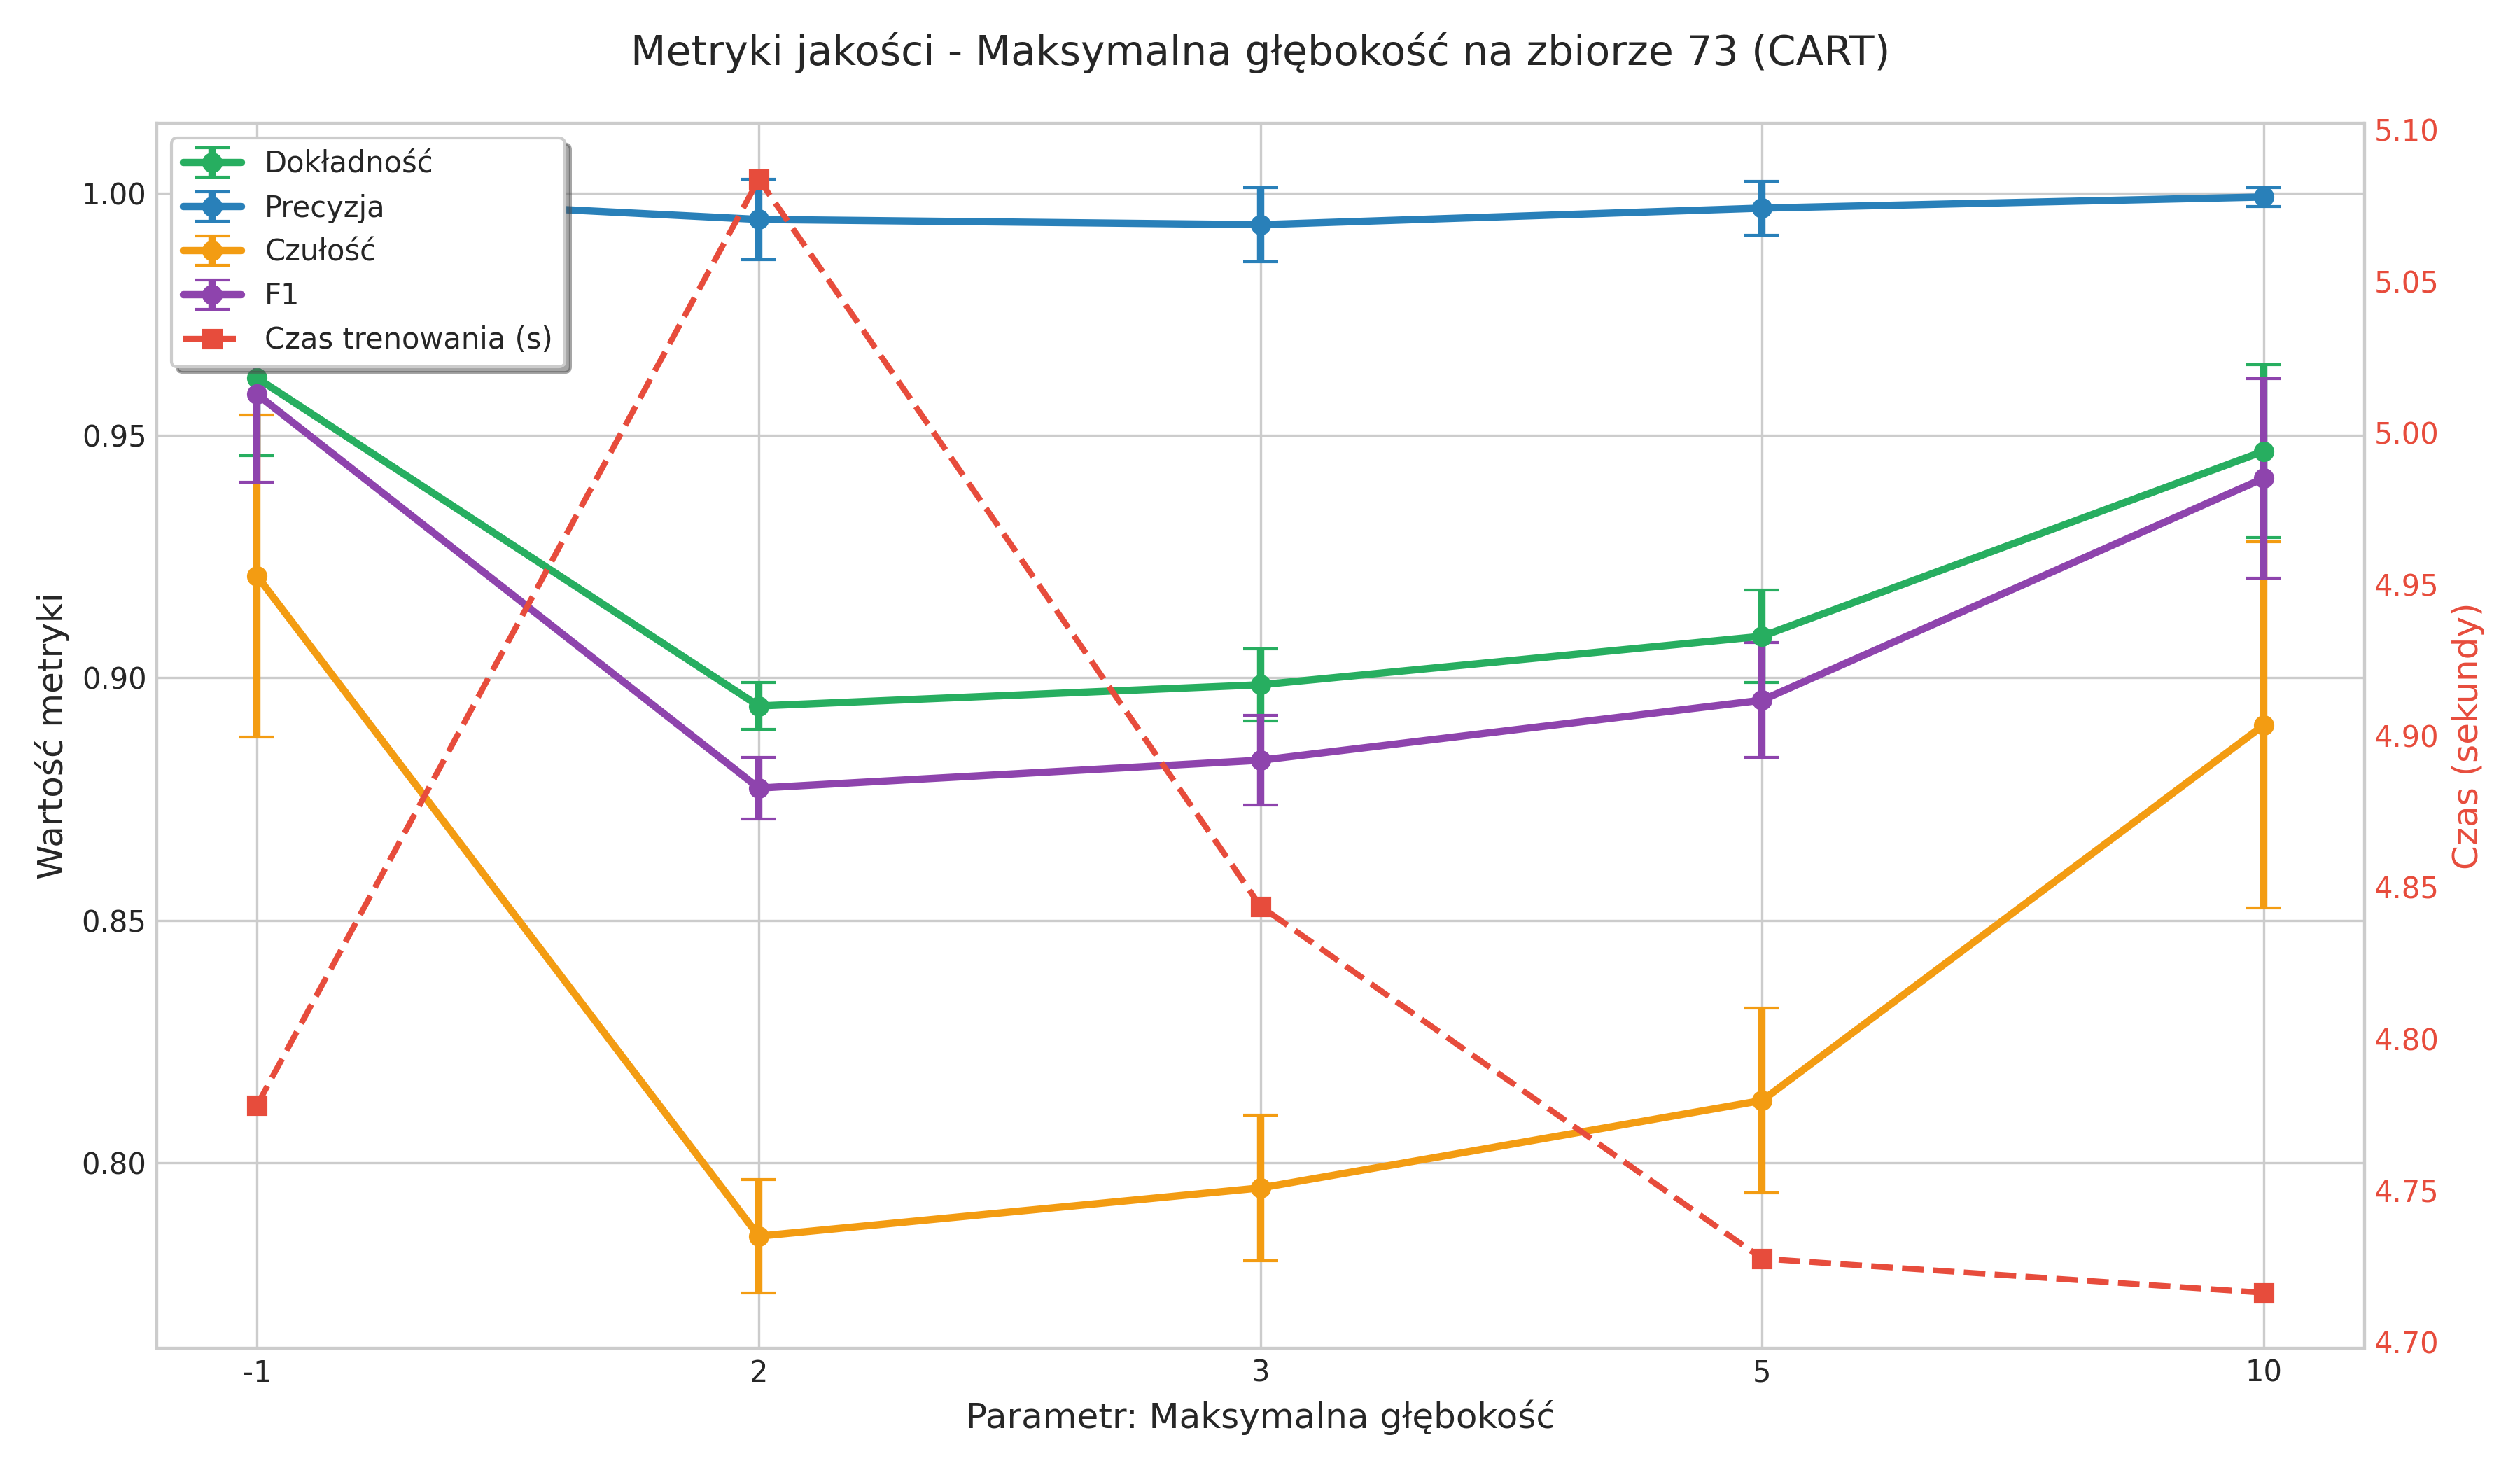
\includegraphics[width=0.9\textwidth]{plots/CART_max_depth_73_metrics.png}
        \caption{Wpływ maksymalnej głębokości na dokładność modelu CART dla zbioru 73 - Grzyby.}
        \label{fig:cart_max_depth_73}
    \end{figure}

    \item Zbiór 14 - Nawrót raka piersi

    Wzrost głębokości początkowo poprawia wyniki modelu, a powyżej głębokości równej 5 obserwujemy brak dalszej poprawy.

    \begin{figure}[H]
        \centering
        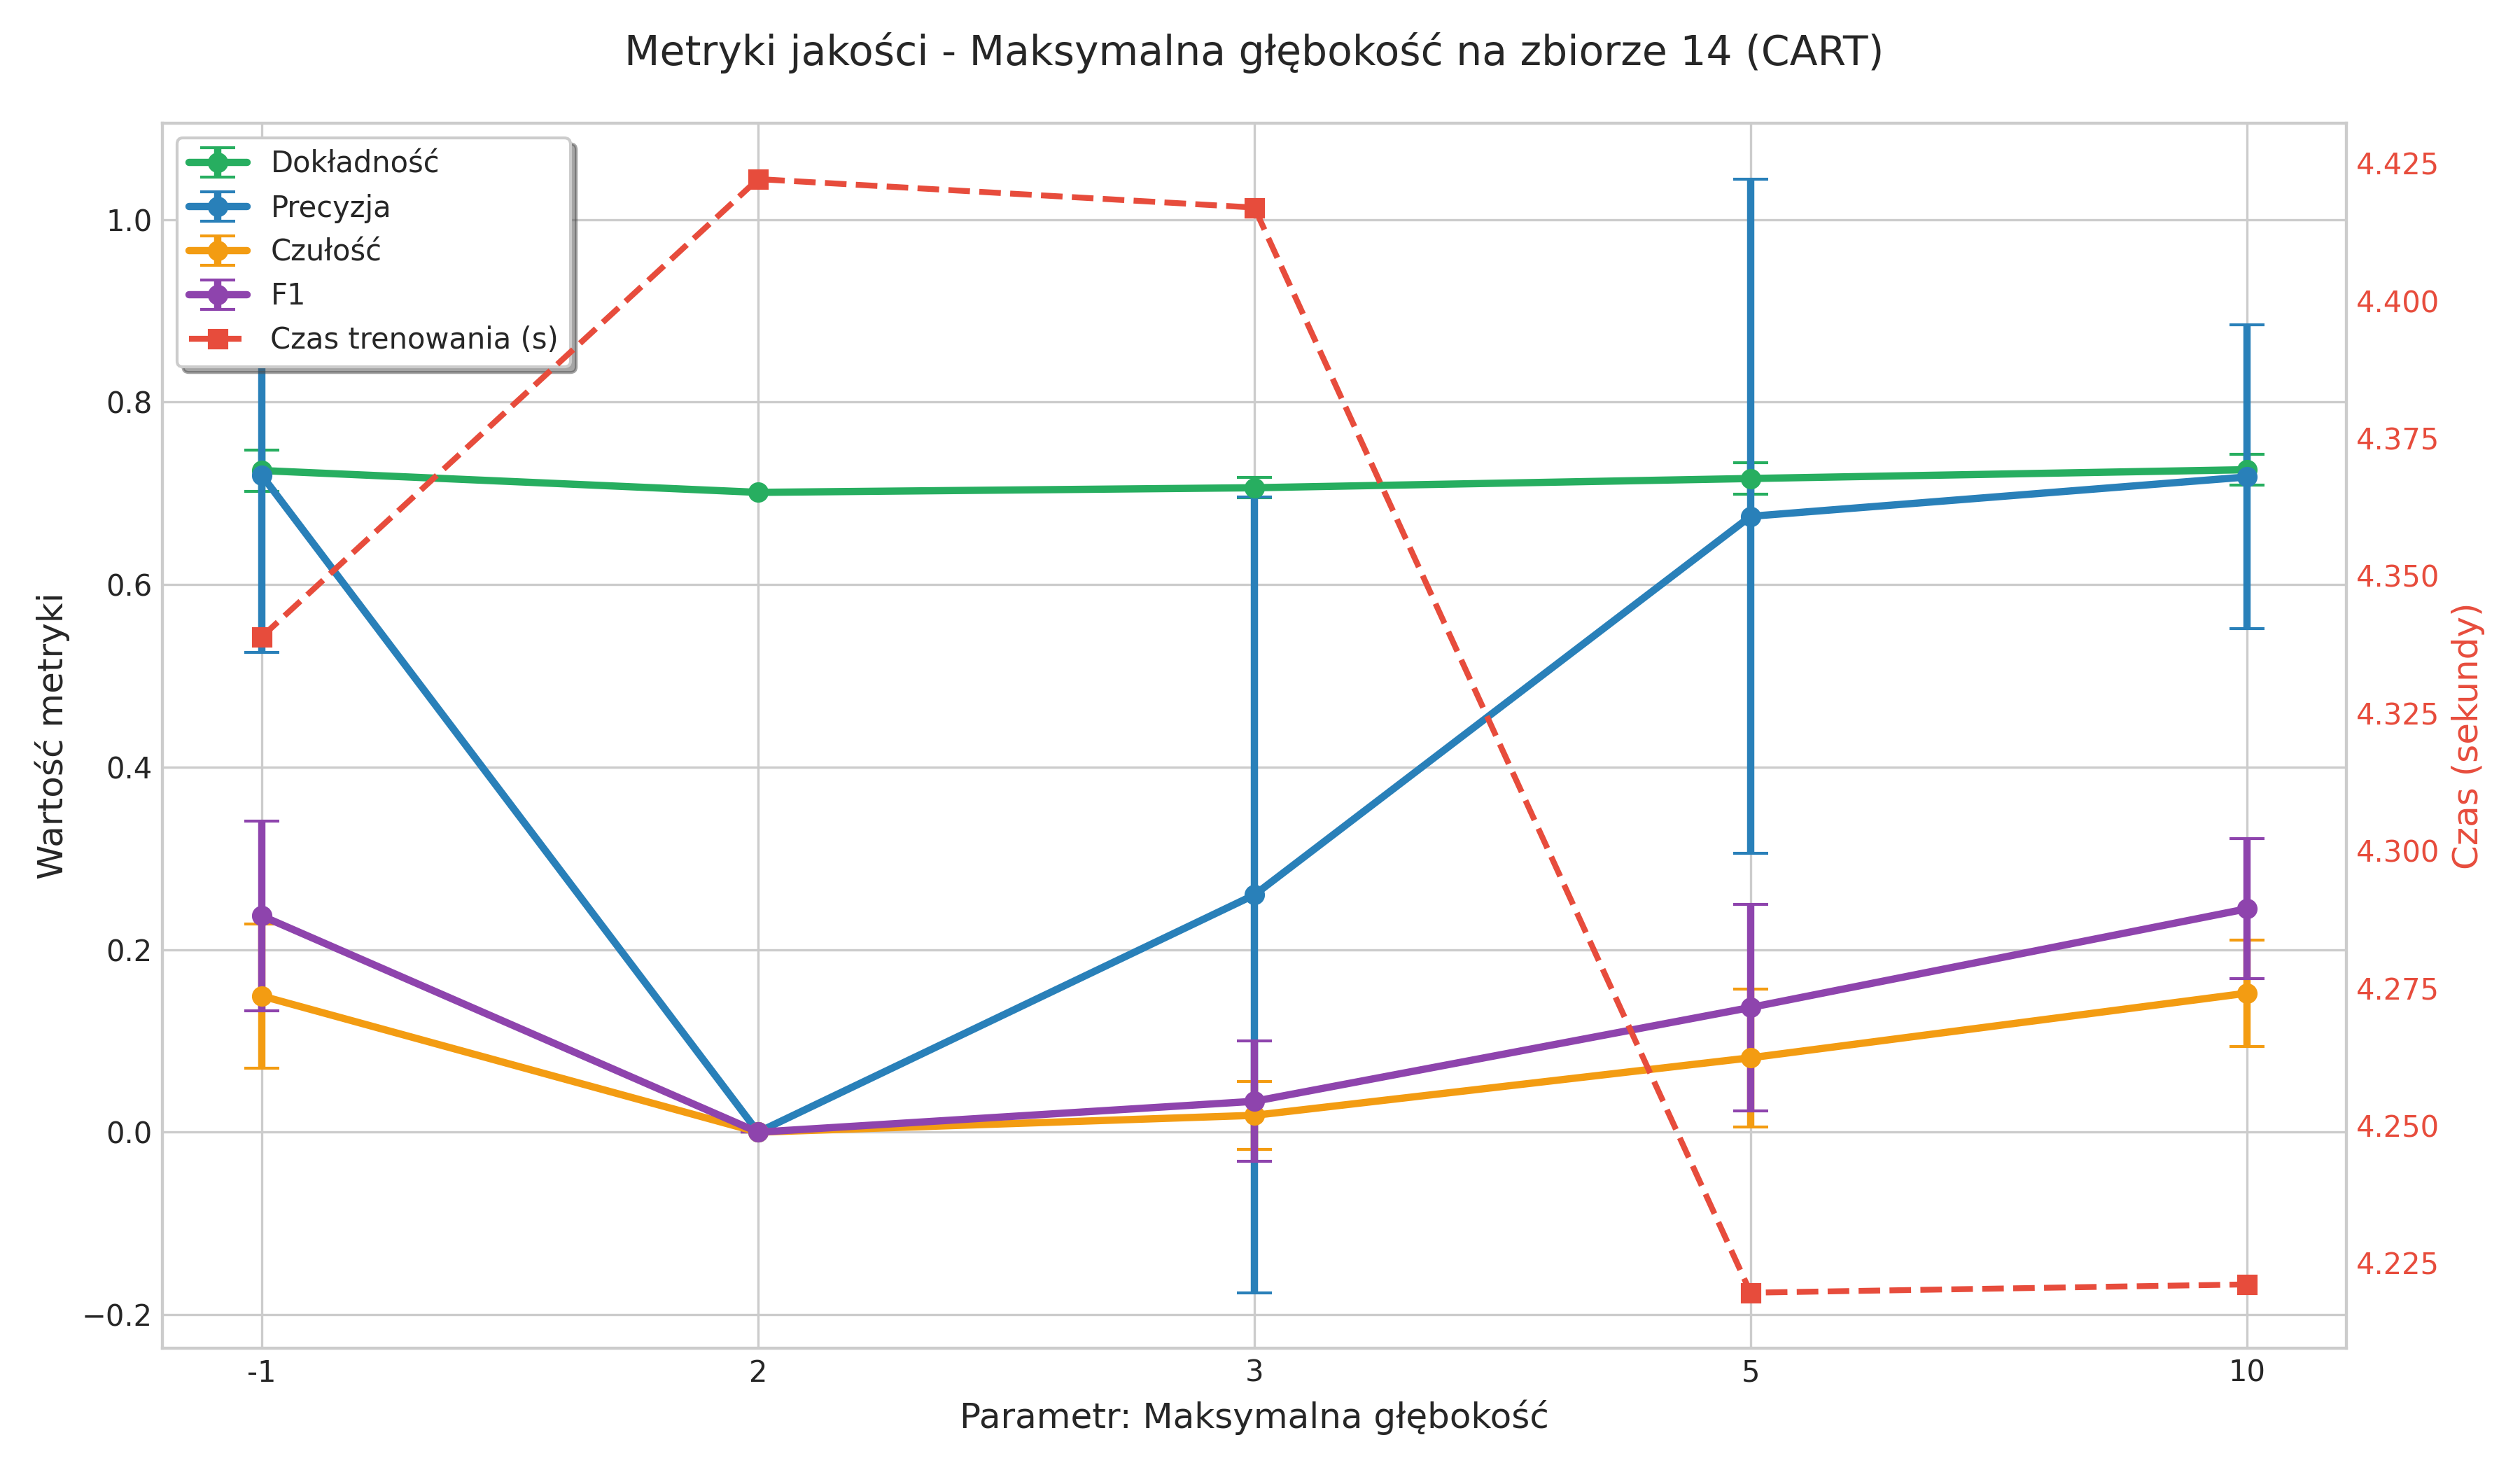
\includegraphics[width=0.9\textwidth]{plots/CART_max_depth_14_metrics.png}
        \caption{Wpływ maksymalnej głębokości na dokładność modelu CART dla zbioru 14 - Nawrót raka piersi.}
        \label{fig:cart_max_depth_14}
    \end{figure}

    \item Zbiór 222 - Skuteczność marketingu bankowego

    Przy głębokości drzew mniejszej niż 10 model zachowuje się całkowicie jak klasyfikator naiwny zawsze przewidujący klasę negatywną.
    Trudniejsze zbiory wymagają głębszych drzew do skutecznej separacji klas.

    \begin{figure}[H]
        \centering
        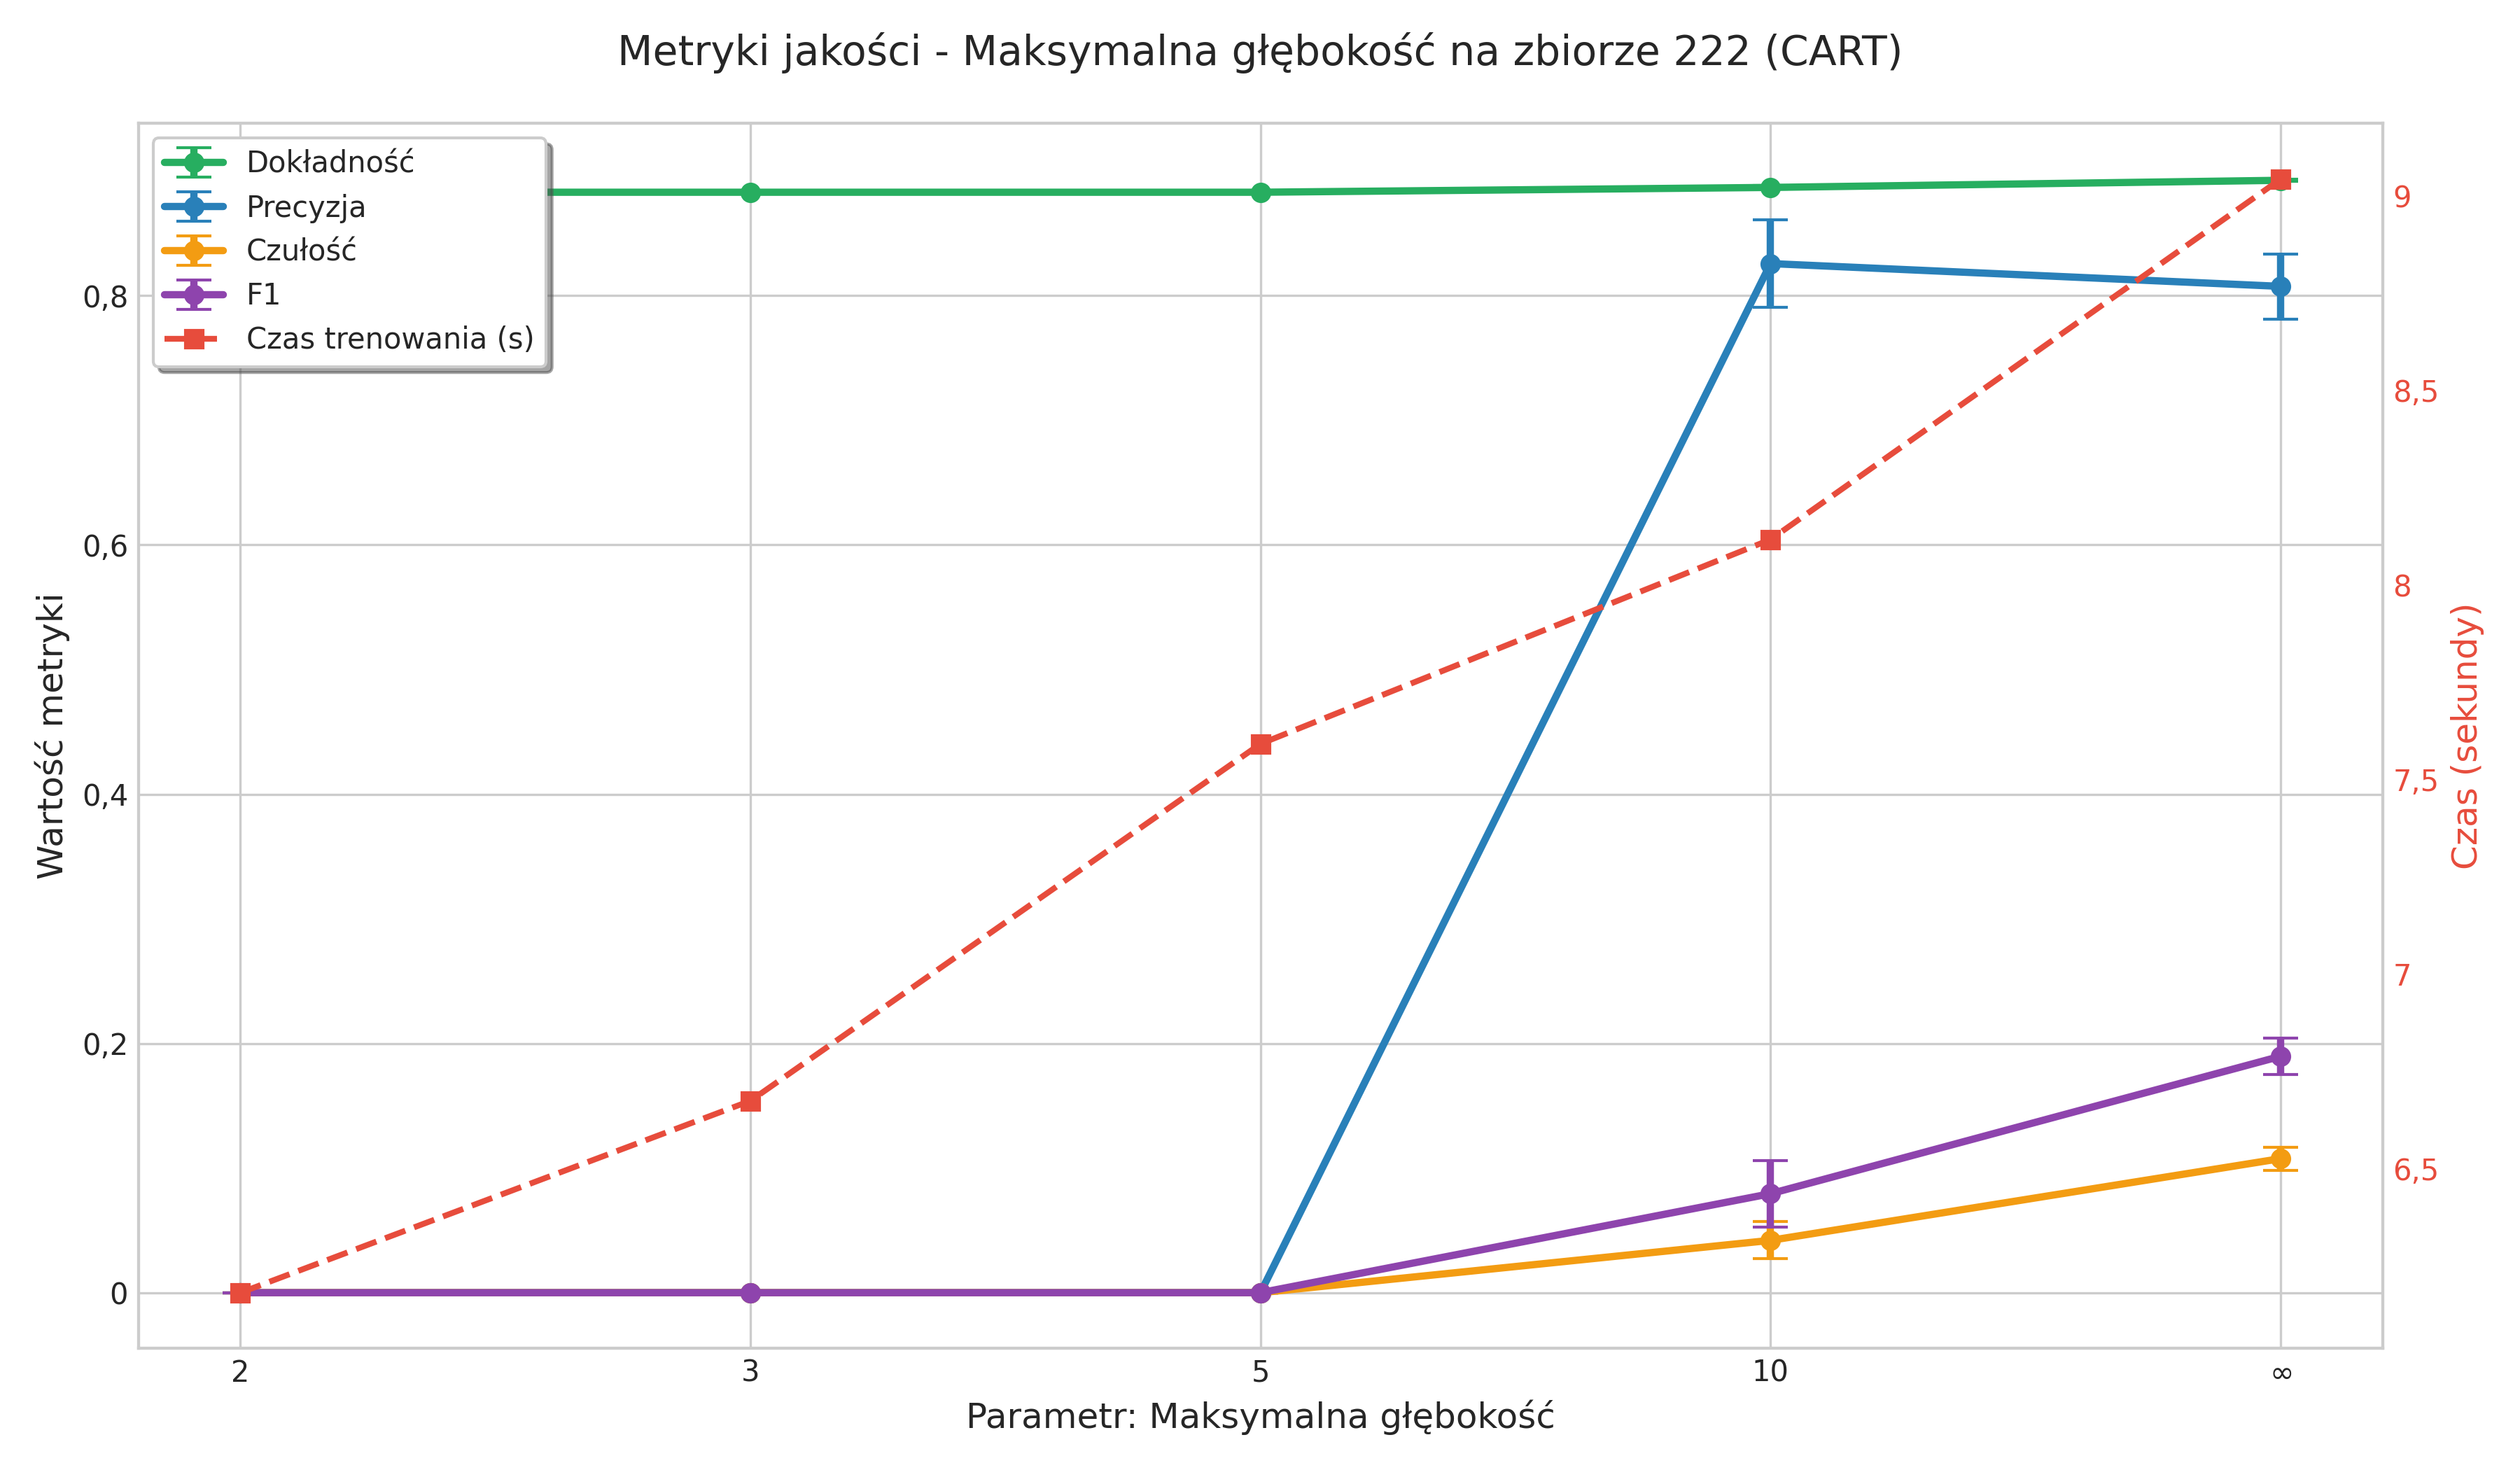
\includegraphics[width=0.9\textwidth]{plots/CART_max_depth_222_metrics.png}
        \caption{Wpływ maksymalnej głębokości na dokładność modelu CART dla zbioru 222 - Skuteczność marketingu bankowego.}
        \label{fig:cart_max_depth_222}
    \end{figure}

    \item Zbiór 350 - Zaległości płatnicze klientów kart kredytowych

    Podobnie jak w pozostałych przypadkach, wzrost maksymalnej głębokości drzew przekłada się na poprawę wyników modelu.

    \begin{figure}[H]
        \centering
        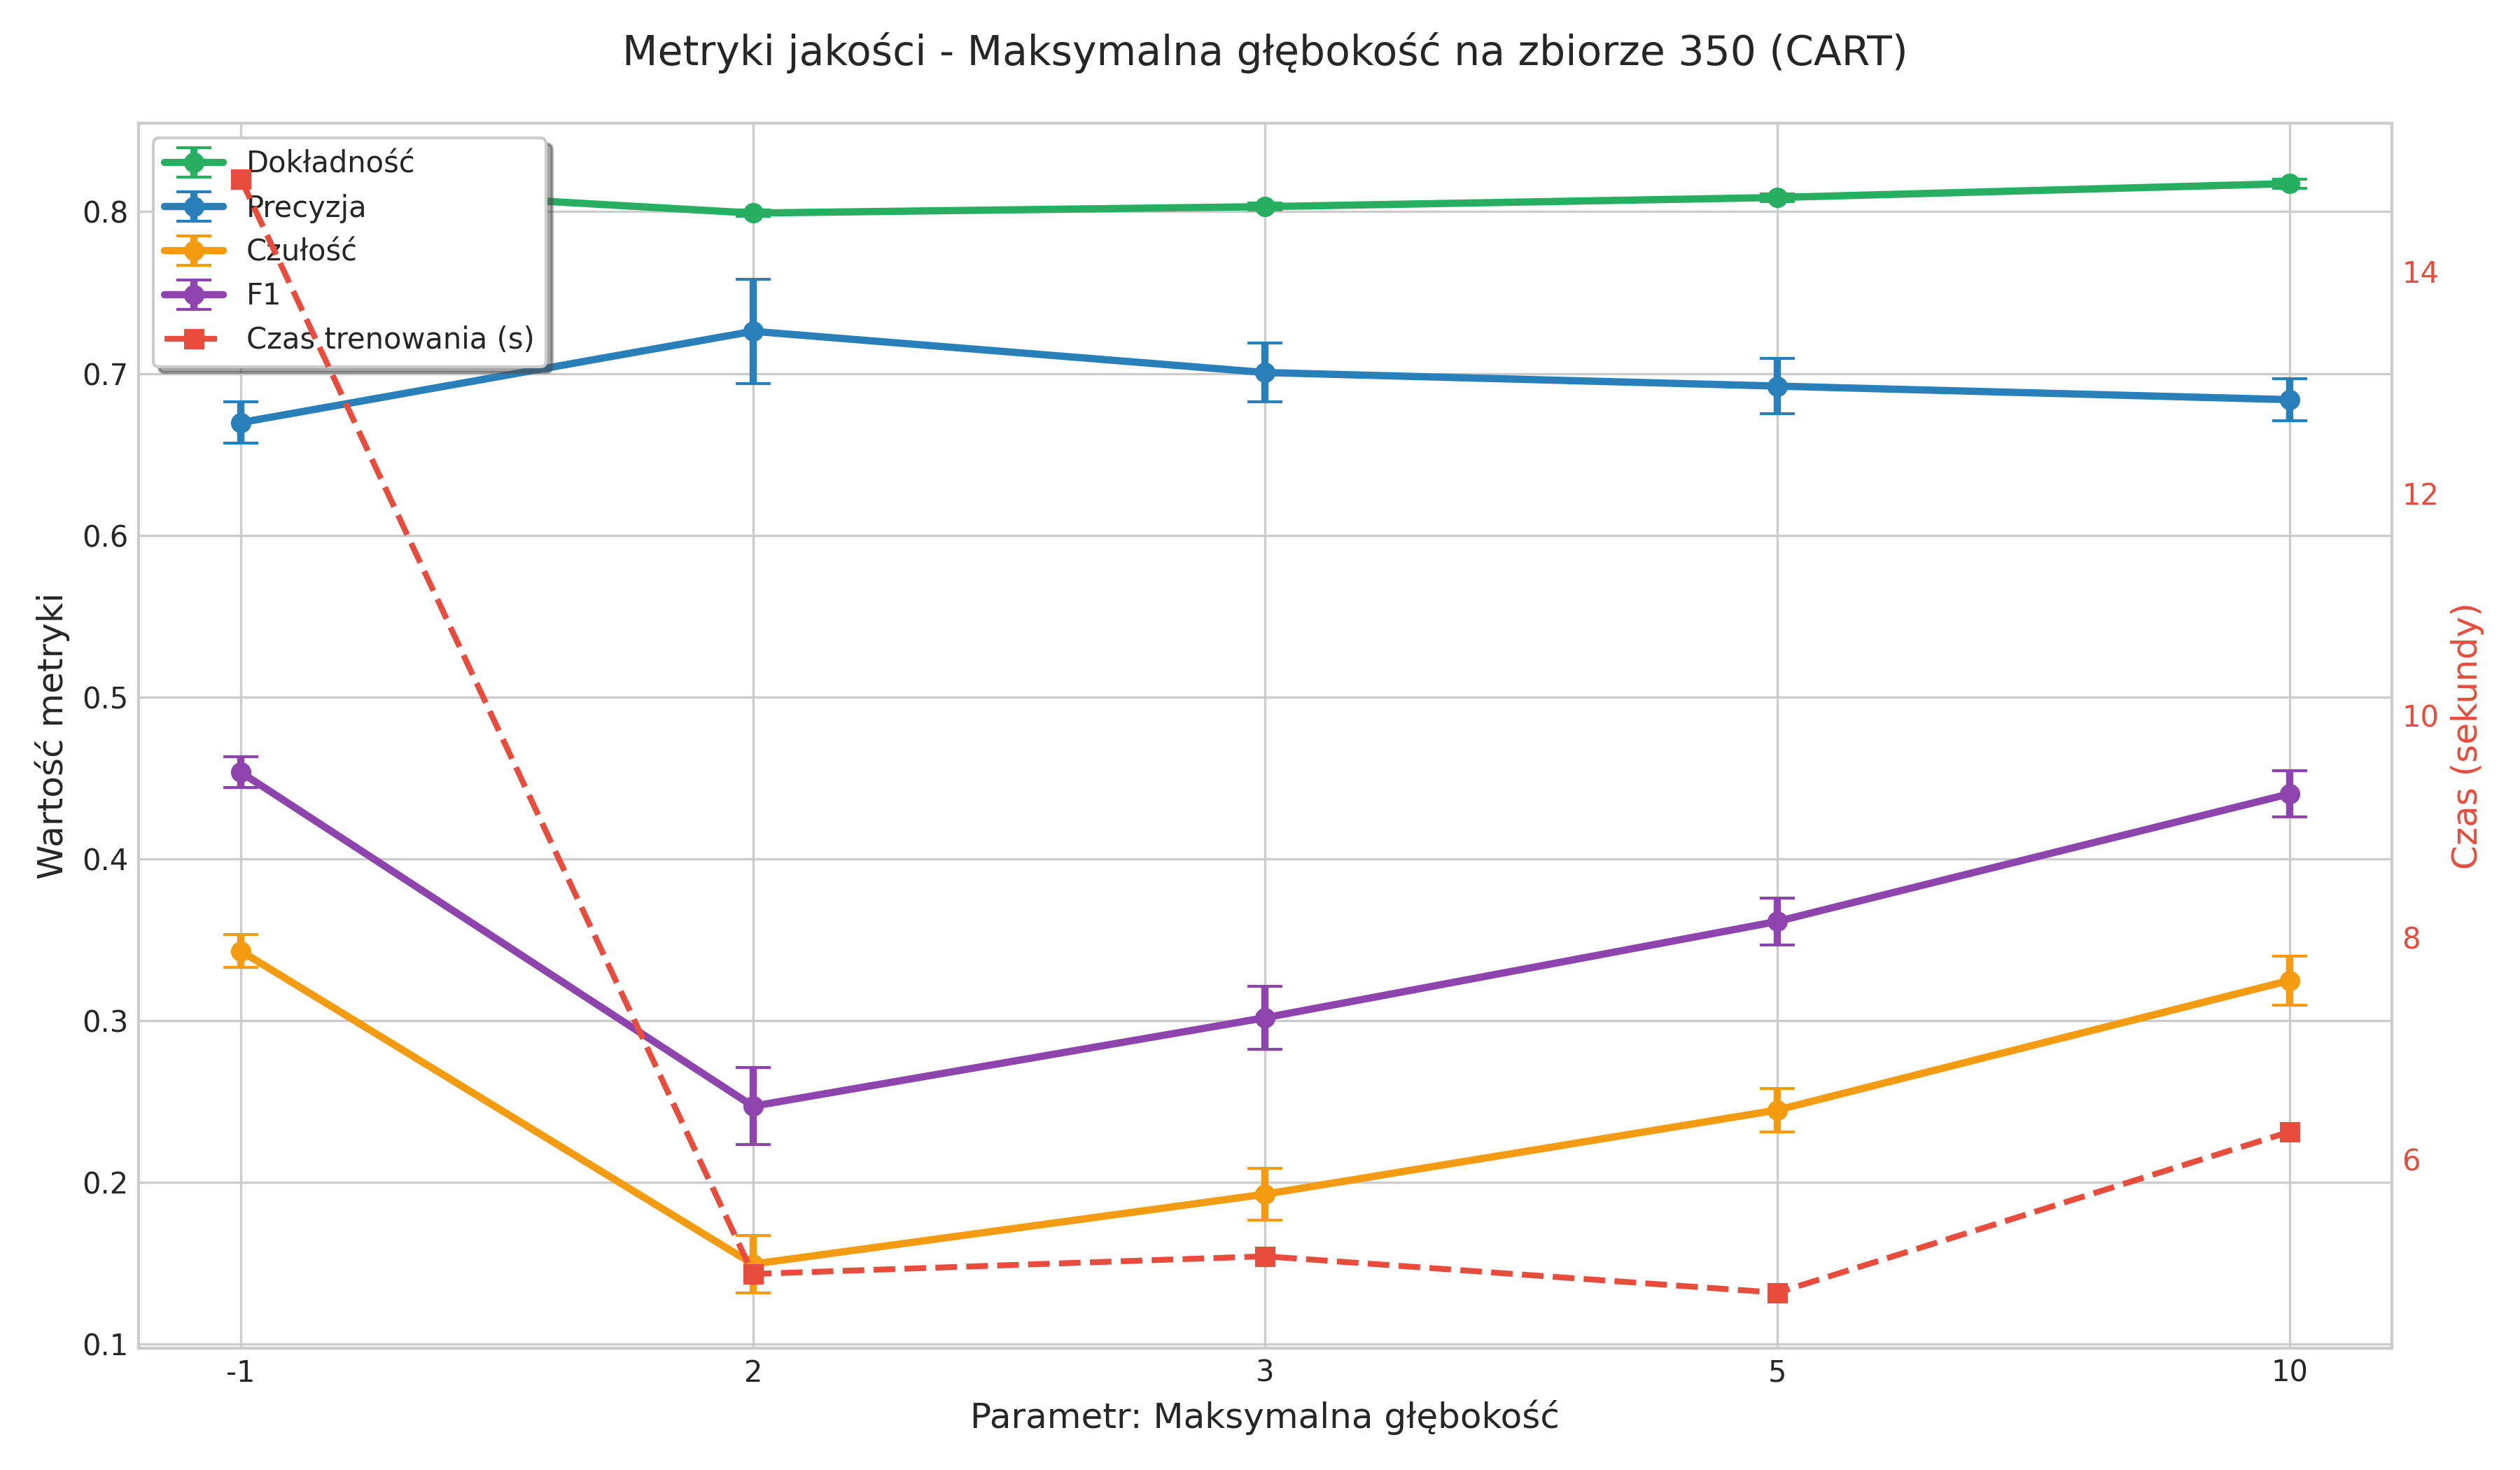
\includegraphics[width=0.9\textwidth]{plots/CART_max_depth_350_metrics.png}
        \caption{Wpływ maksymalnej głębokości na dokładność modelu CART dla zbioru 350 - Zaległości płatnicze klientów kart kredytowych.}
        \label{fig:cart_max_depth_350}
    \end{figure}
\end{itemize}

\subsubsection{Wnioski ogólne}
\begin{itemize}
    \item Wyniki wskazują, że stosowanie ograniczenia maksymalnej głębokości drzew nie jest uzasadnione na badanych zbiorach danych.
    \item W porównywaniu modeli zostanie utrzymany brak ograniczenia maksymalnej głębokości drzew.
\end{itemize}

\subsection{Rozmiar turnieju}

\subsubsection{ID3}
\begin{itemize}
    \item Zbiór 73 - Grzyby

    Zbiór jest na tyle trywialny, że nawet losowy wybór cech podziału węzła (turniej o rozmiarze 1) pozwala na osiągnięcie 100\% dokładności.

    \begin{figure}[H]
        \centering
        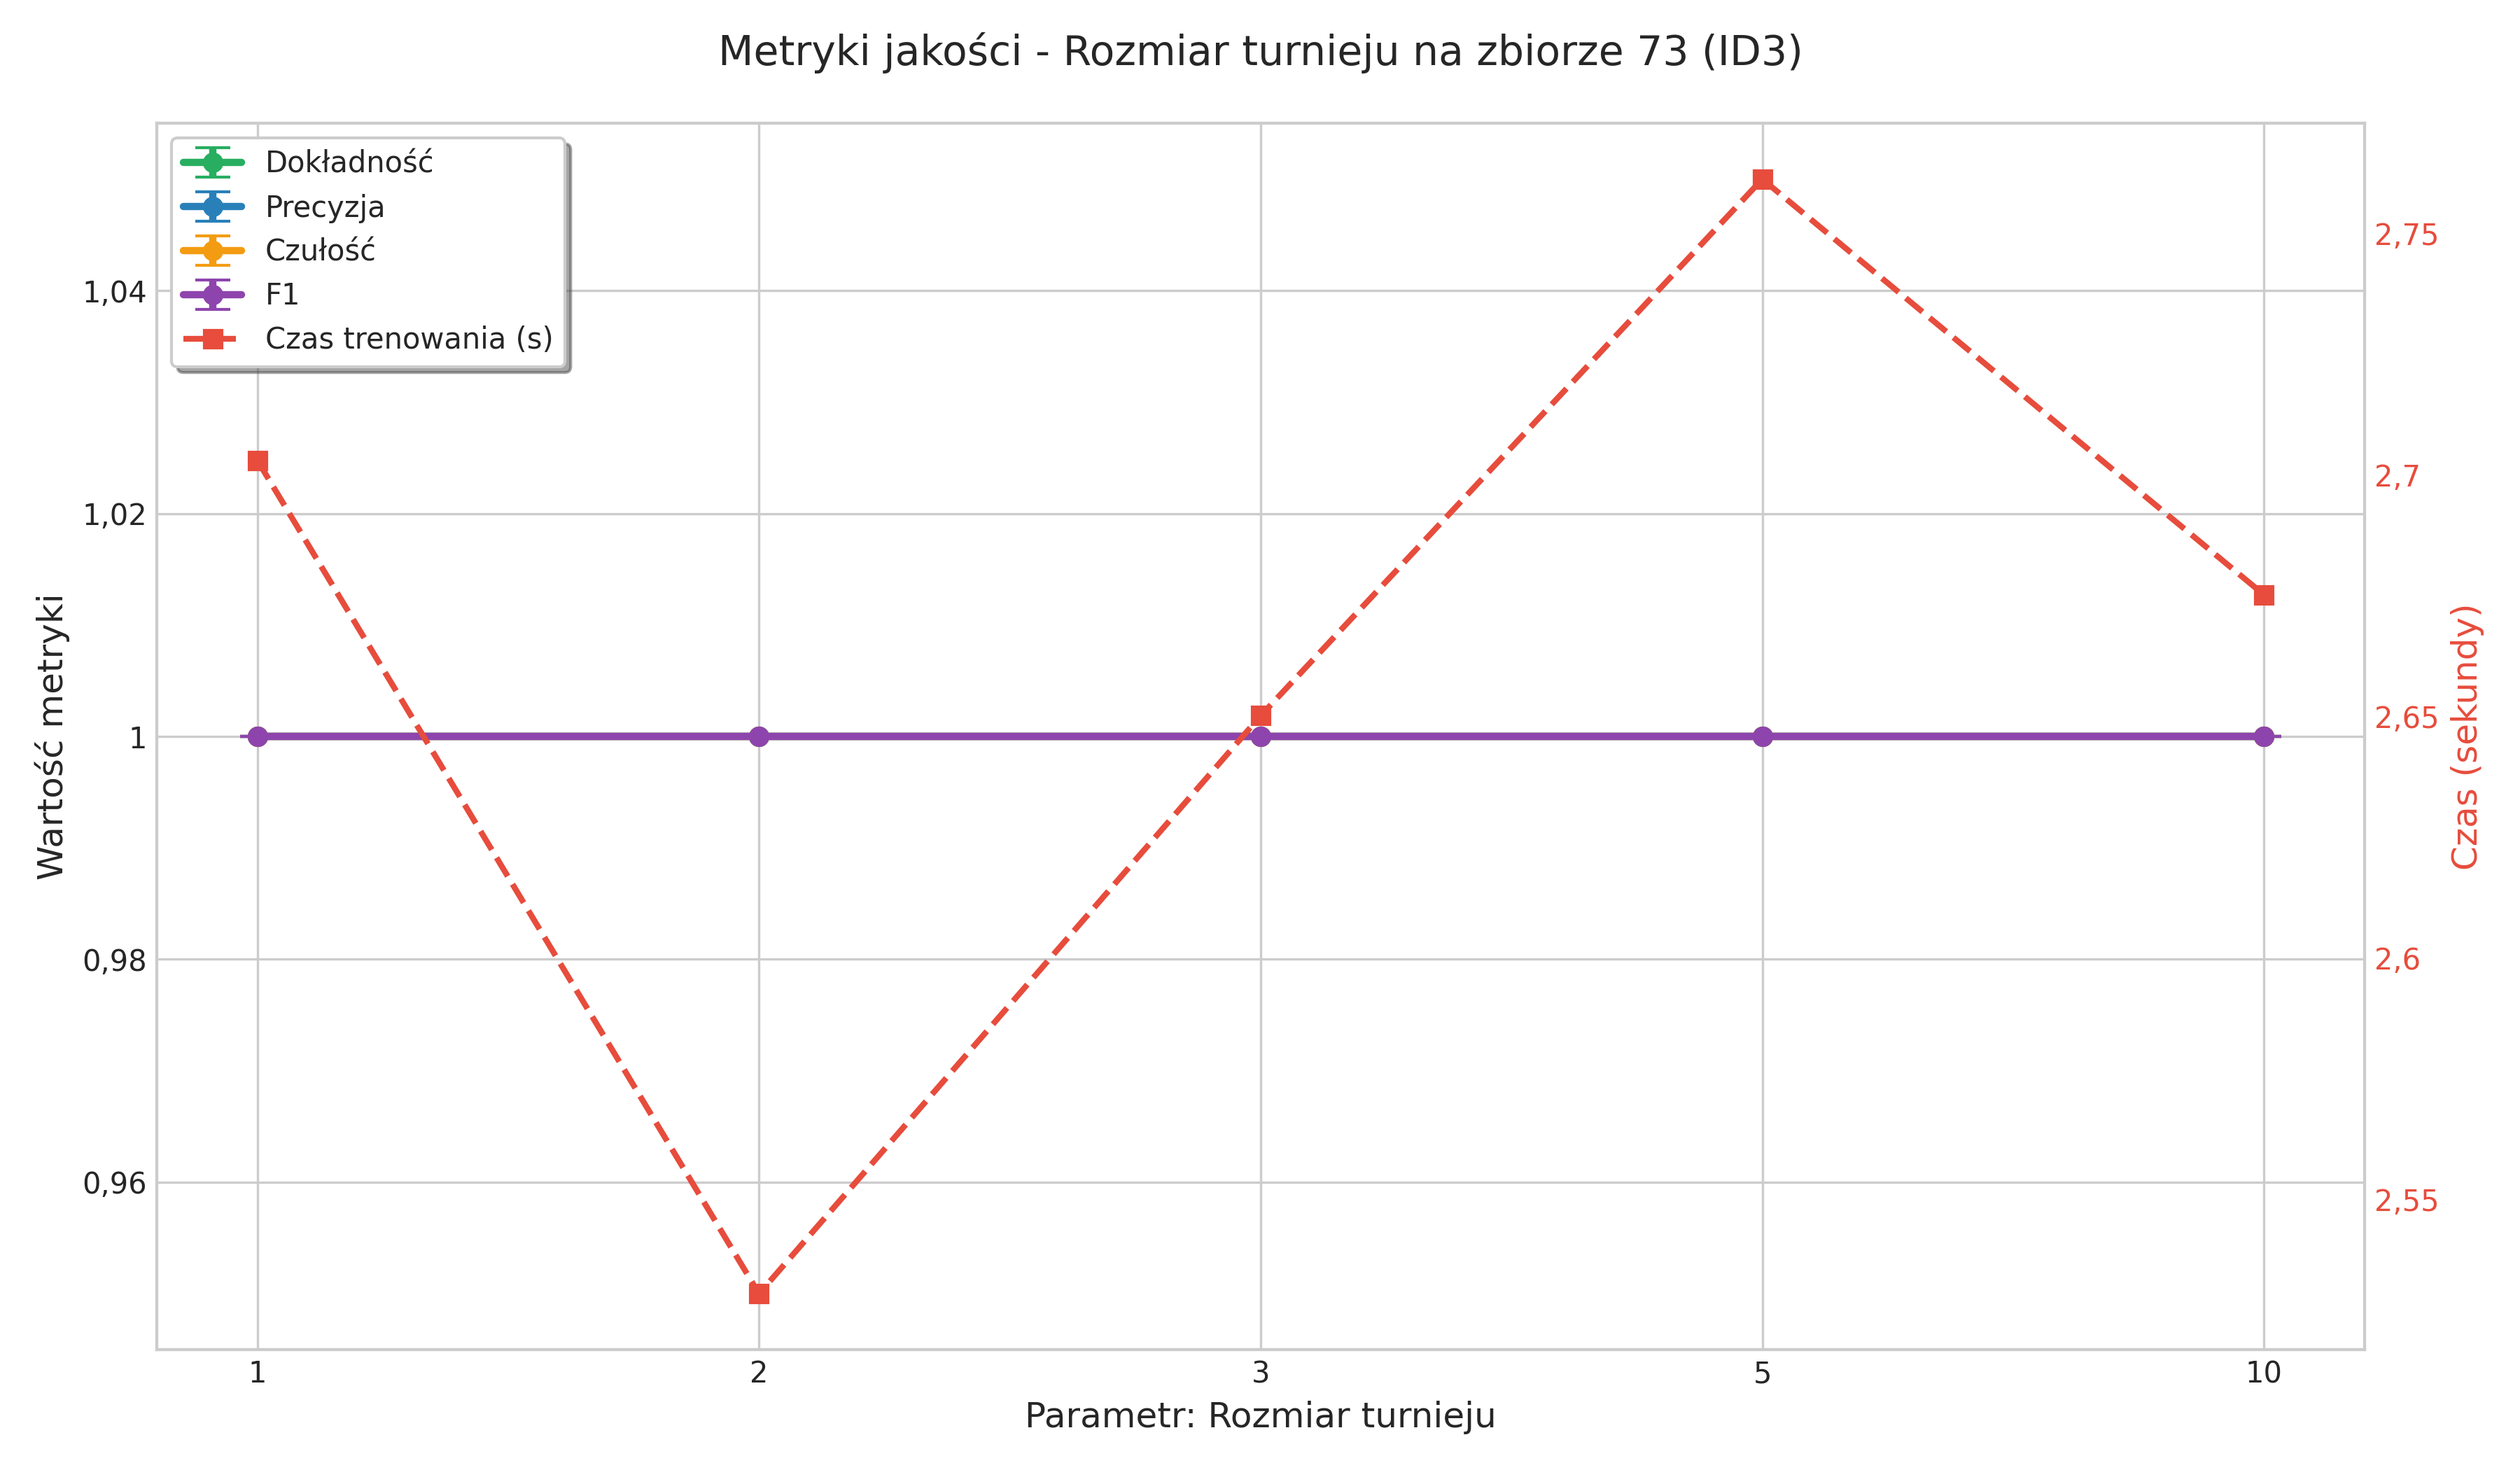
\includegraphics[width=0.9\textwidth]{plots/ID3_tournament_size_73_metrics.png}
        \caption{Wpływ rozmiaru turnieju na dokładność modelu ID3 dla zbioru 73 - Grzyby.}
        \label{fig:id3_tournament_size_73}
    \end{figure}

    \item Zbiór 14 - Nawrót raka piersi

    Obserwujemy spadek dokładności wraz ze wzrostem liczebności turnieju. Przykłady z tego zbioru posiadają niewiele atrybutów, przez co
    ustawienie wielkości turnieju na 10 prowadzi do bardzo małej różnorodności drzew w lesie i wzrostu wariancji modelu oraz przeuczenia.

    \begin{figure}[H]
        \centering
        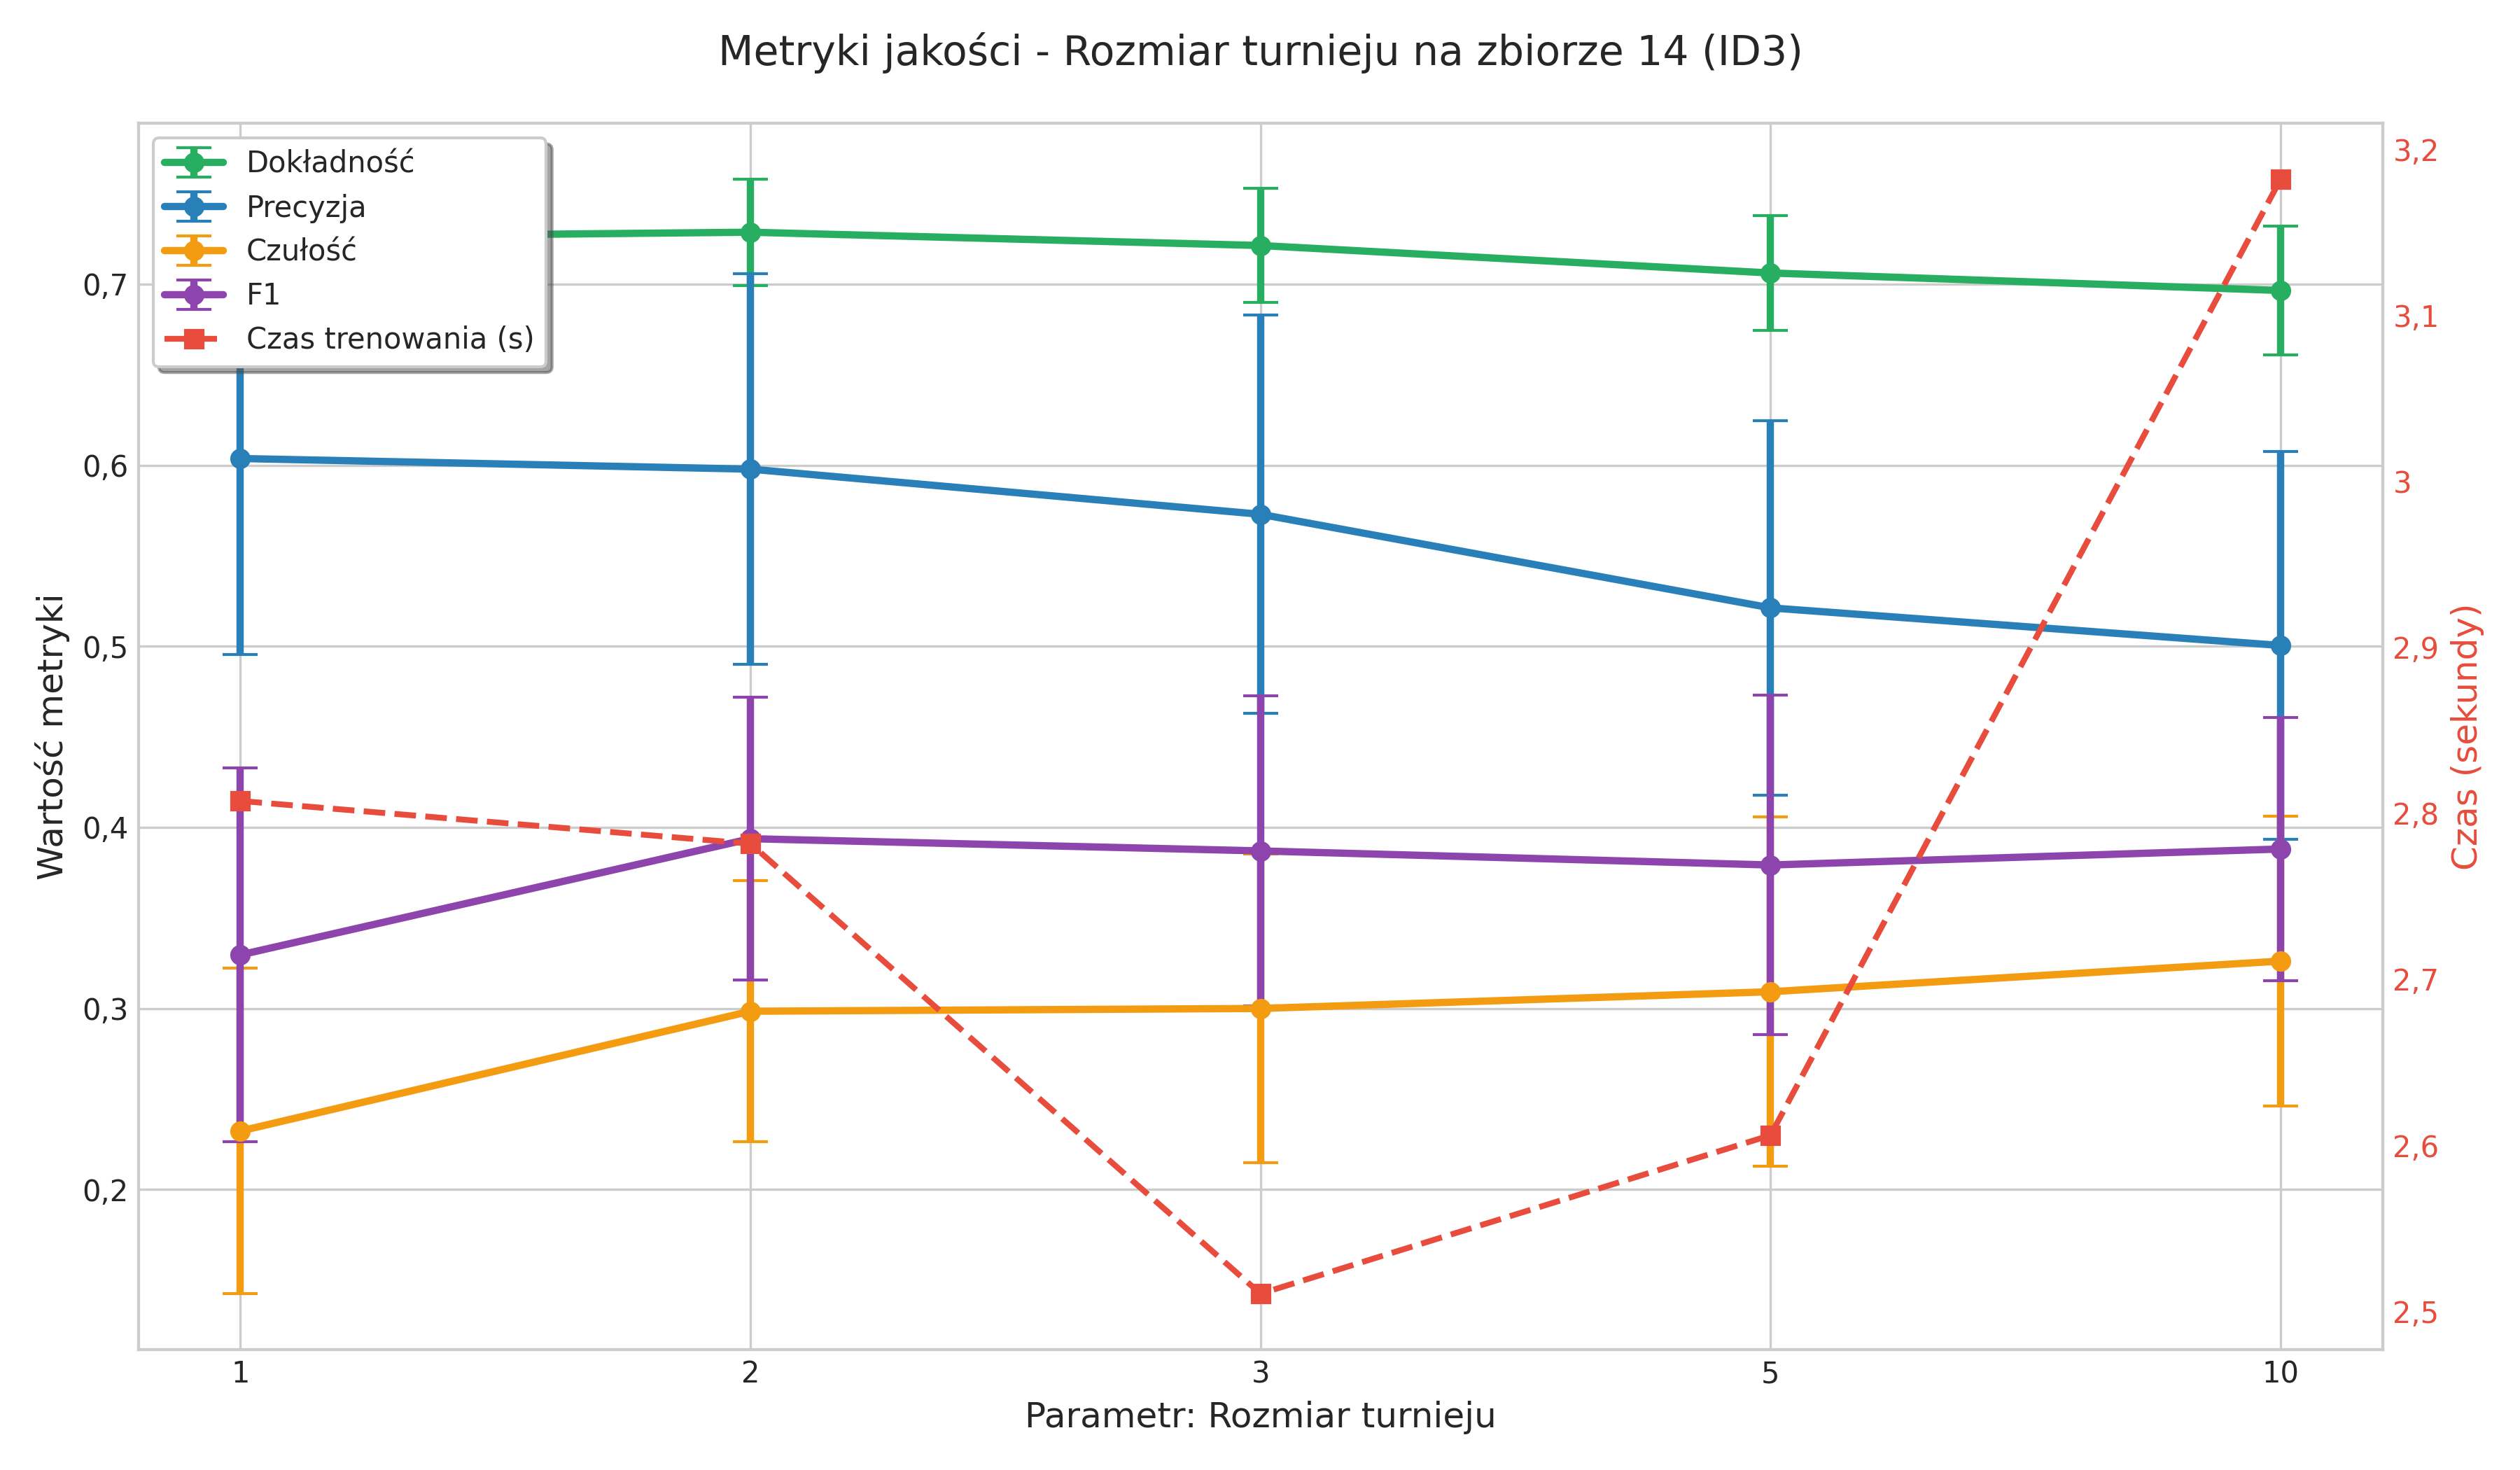
\includegraphics[width=0.9\textwidth]{plots/ID3_tournament_size_14_metrics.png}
        \caption{Wpływ rozmiaru turnieju na dokładność modelu ID3 dla zbioru 14 - Nawrót raka piersi.}
        \label{fig:id3_tournament_size_14}
    \end{figure}

\end{itemize}
\subsubsection{CART}
\begin{itemize}
    \item Zbiór 73 - Grzyby

    W przypadku radzenia sobie ze zwiększoną liczbą atrybutów (one-hot encoding) większy rozmiar turnieju pozwala na
    wybór bardziej reprezentatywnych cech podziału, co przekłada się na lepsze wyniki modelu. Zwiększenie rozmiaru turnieju pozwala
    uniknąć zjawiska niedouczenia drzew.

    \begin{figure}[H]
        \centering
        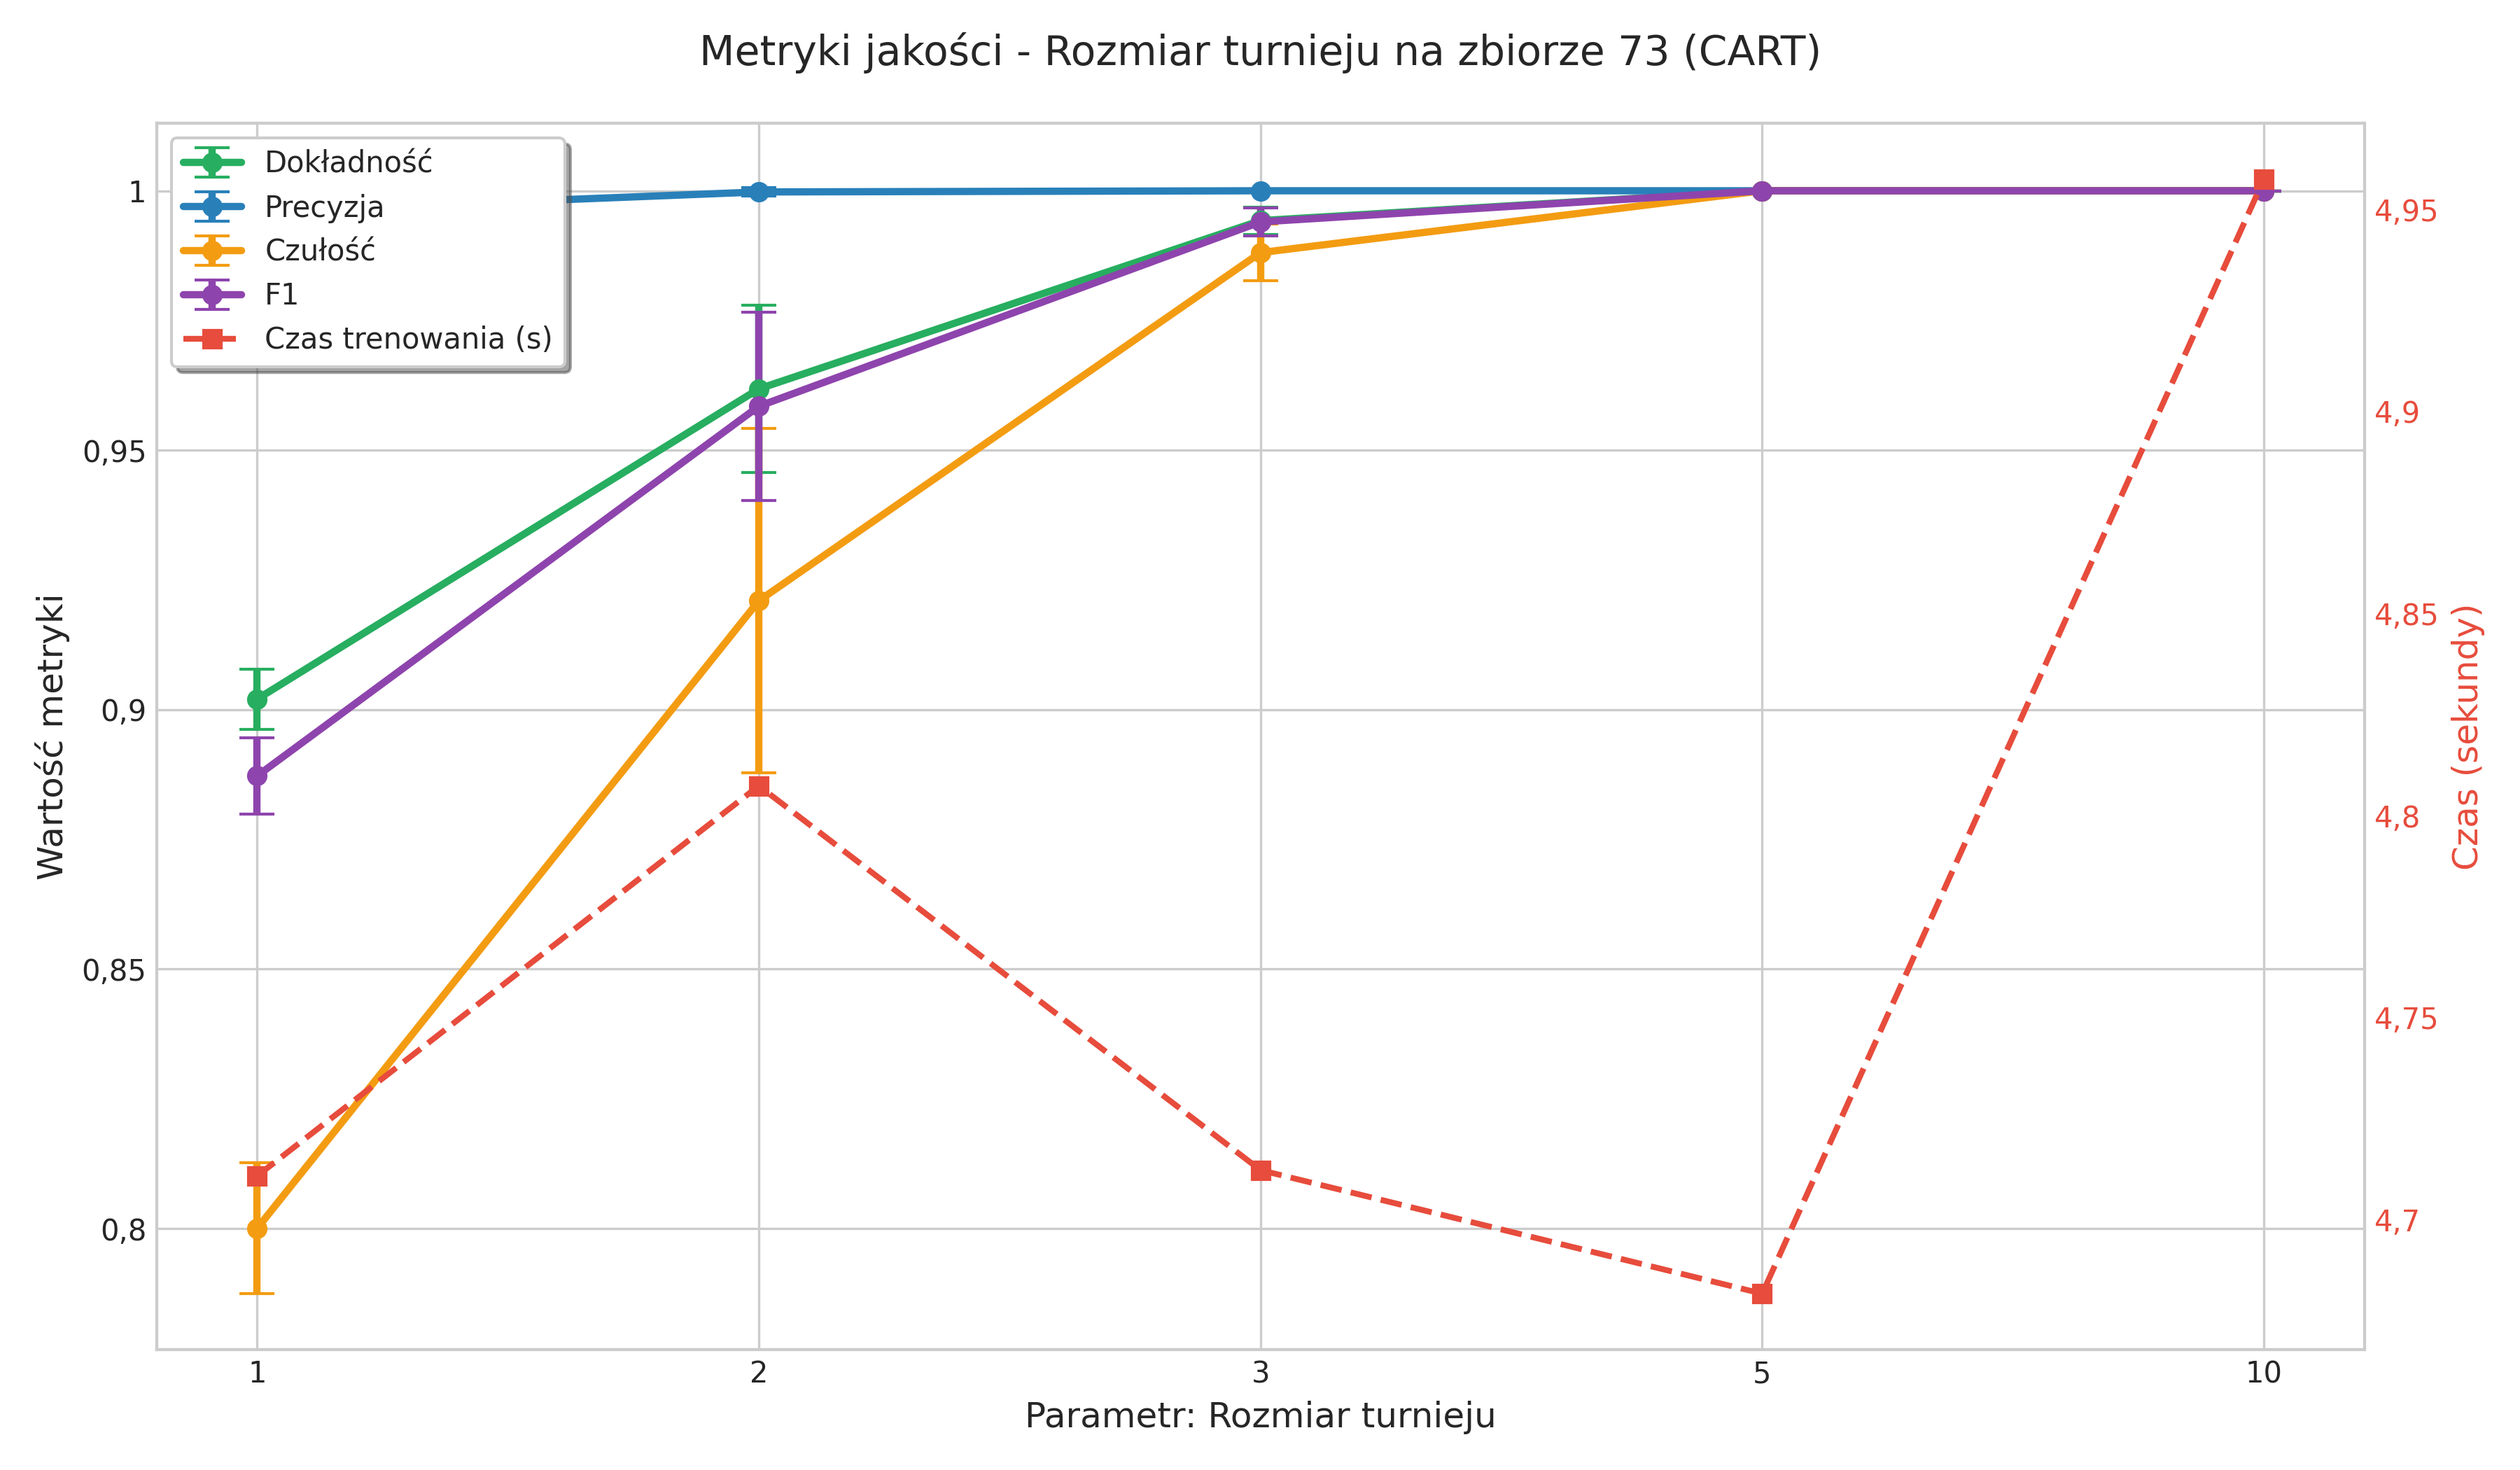
\includegraphics[width=0.9\textwidth]{plots/CART_tournament_size_73_metrics.png}
        \caption{Wpływ rozmiaru turnieju na dokładność modelu CART dla zbioru 73 - Grzyby.}
        \label{fig:cart_tournament_size_73}
    \end{figure}

    \item Zbiór 14 - Nawrót raka piersi

    Wzrost rozmiaru turnieju nie wpływa na dokładność modelu, jednak obserwujemy poprawę czułości oraz F1-score, przy jednoczesnym spadku precyzji.
    Oznacza to, że model przesuwa swój punkt pracy w stronę maksymalizacji wykrywalności.
    Zwiększenie rozmiaru turnieju faworyzuje te podziały w drzewach, które skuteczniej separują klasę mniejszościową (nawrót),
    nawet za cenę częstszego mylenia się na klasie większościowej (zdrowi).

    \begin{figure}[H]
        \centering
        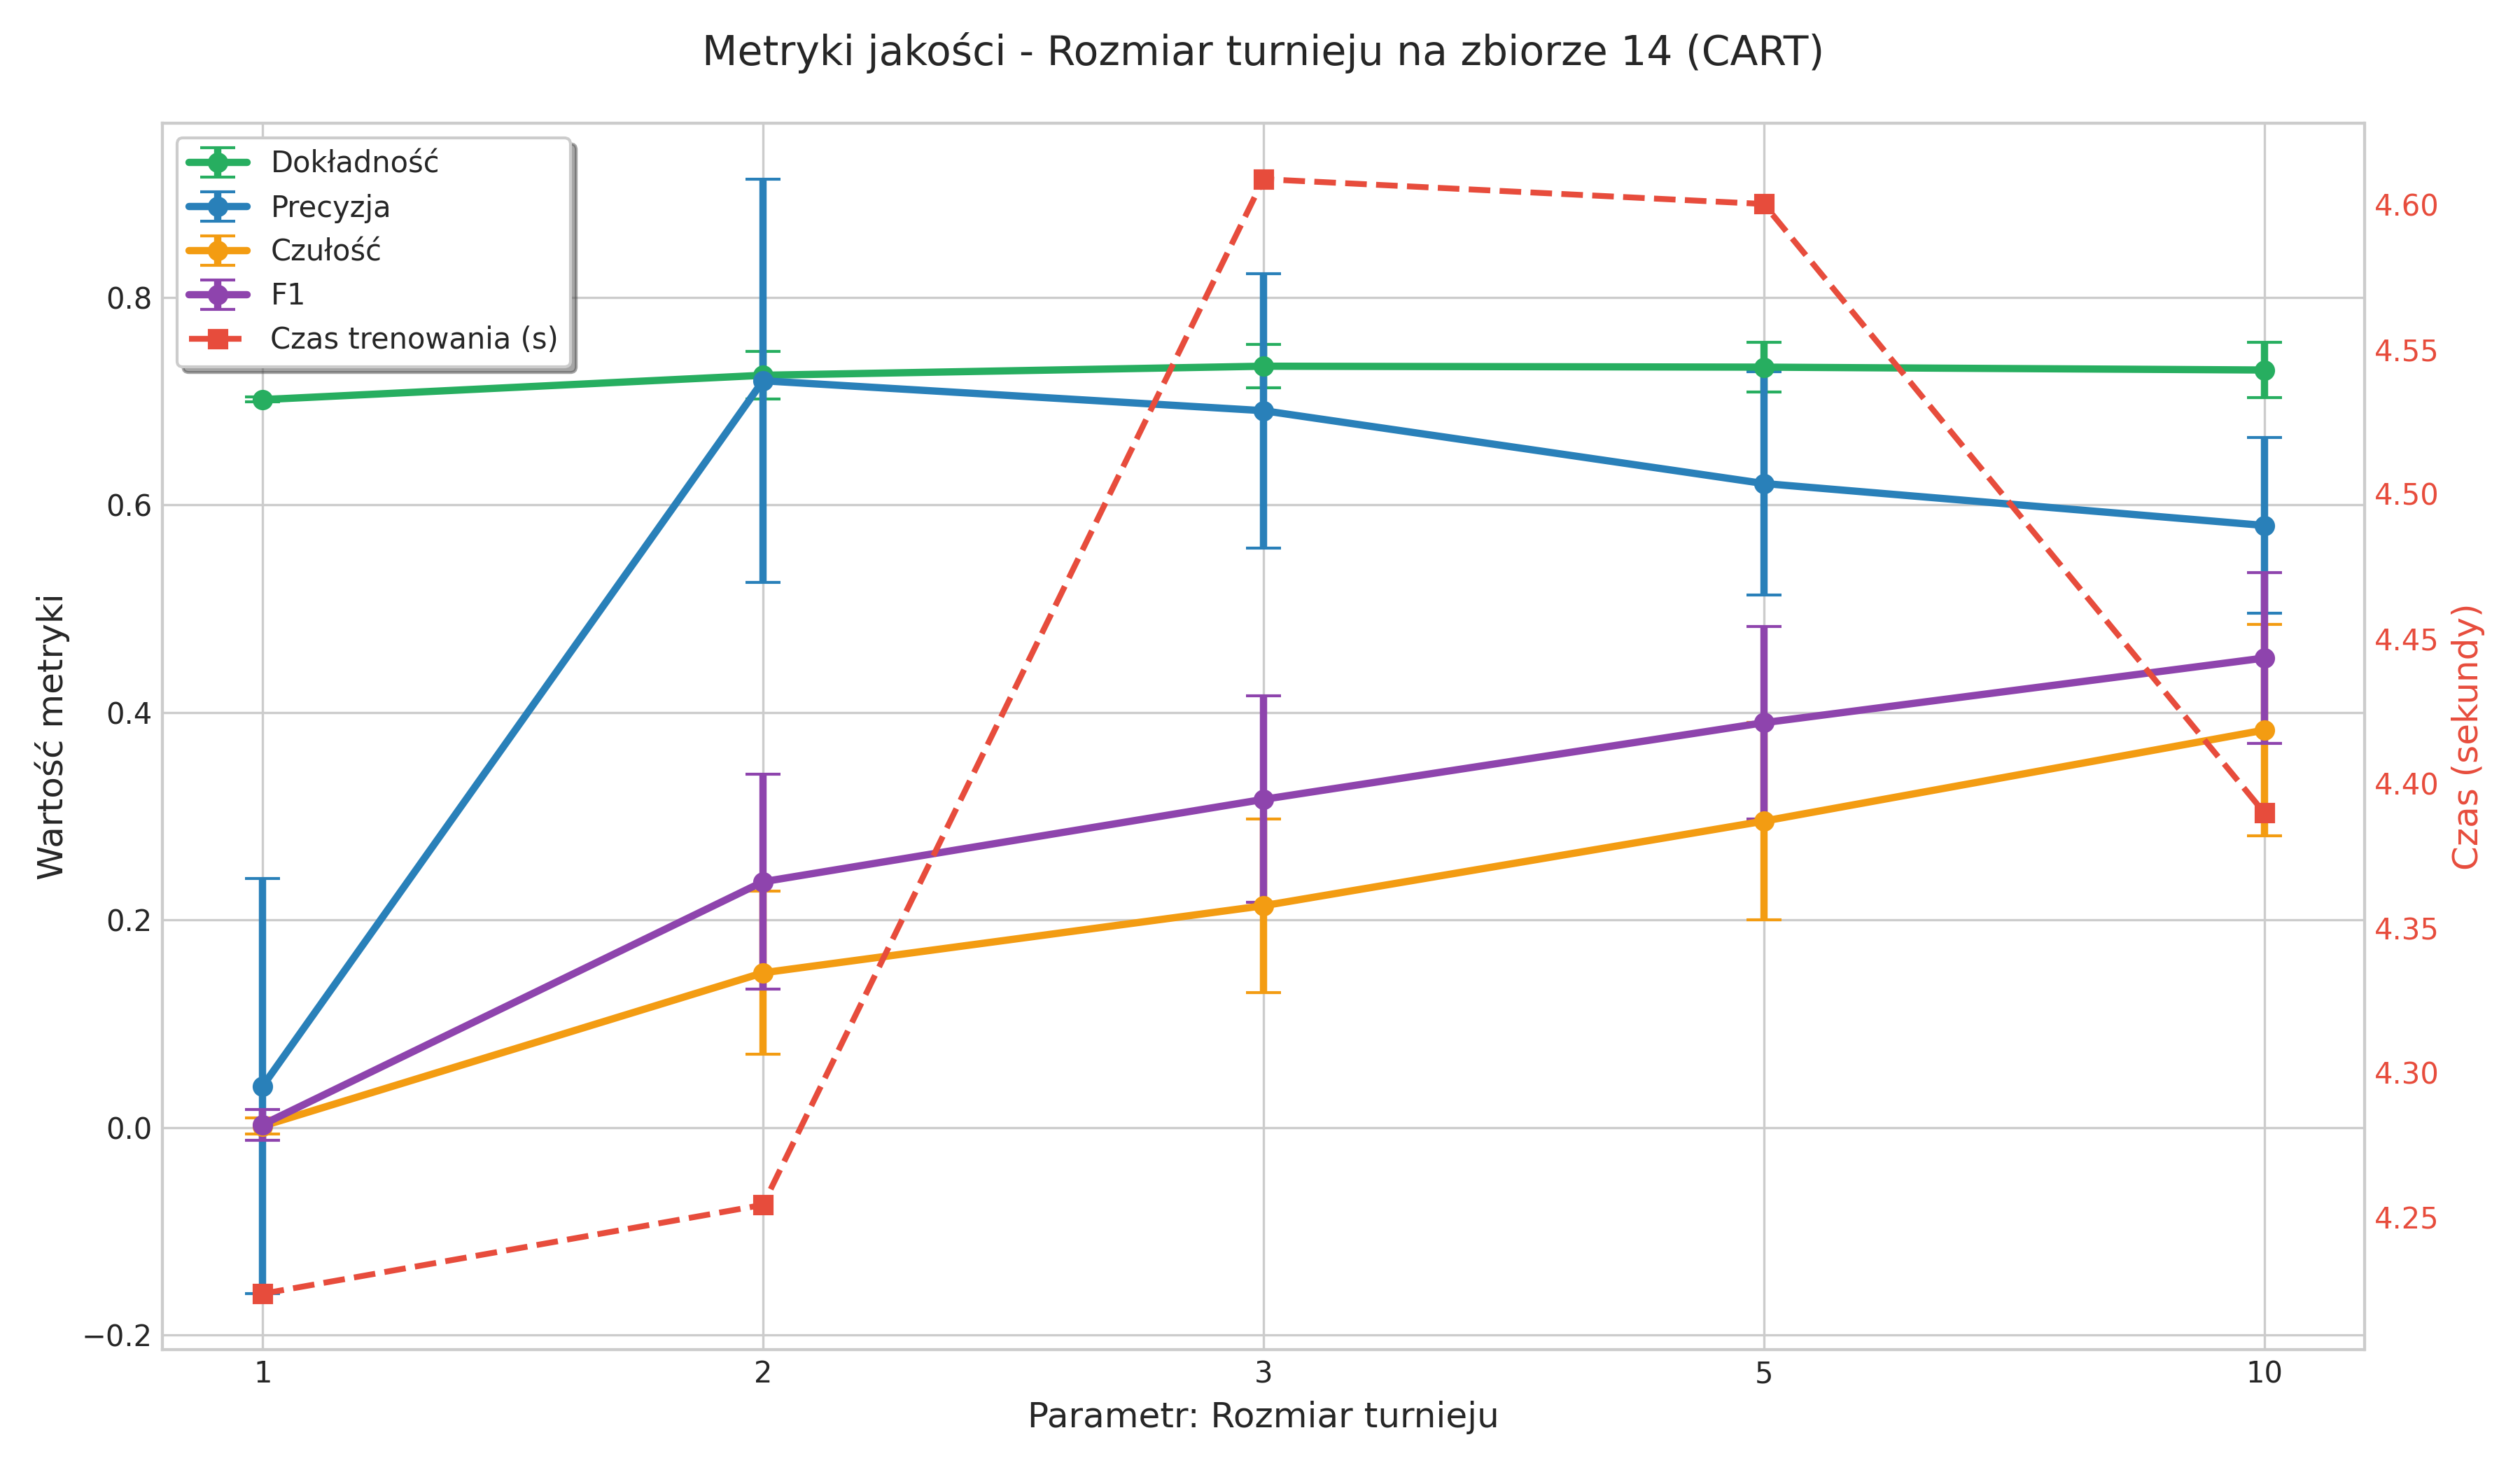
\includegraphics[width=0.9\textwidth]{plots/CART_tournament_size_14_metrics.png}
        \caption{Wpływ rozmiaru turnieju na dokładność modelu CART dla zbioru 14 - Nawrót raka piersi.}
        \label{fig:cart_tournament_size_14}
    \end{figure}

    \item Zbiór 222 - Skuteczność marketingu bankowego

    Obserwacje są podobne jak dla zbioru 14. Dodatkowo warto zauważyć, że wraz ze wzrostem rozmiaru turnieju znacząco rośnie czas trenowania lasu.

    \begin{figure}[H]
        \centering
        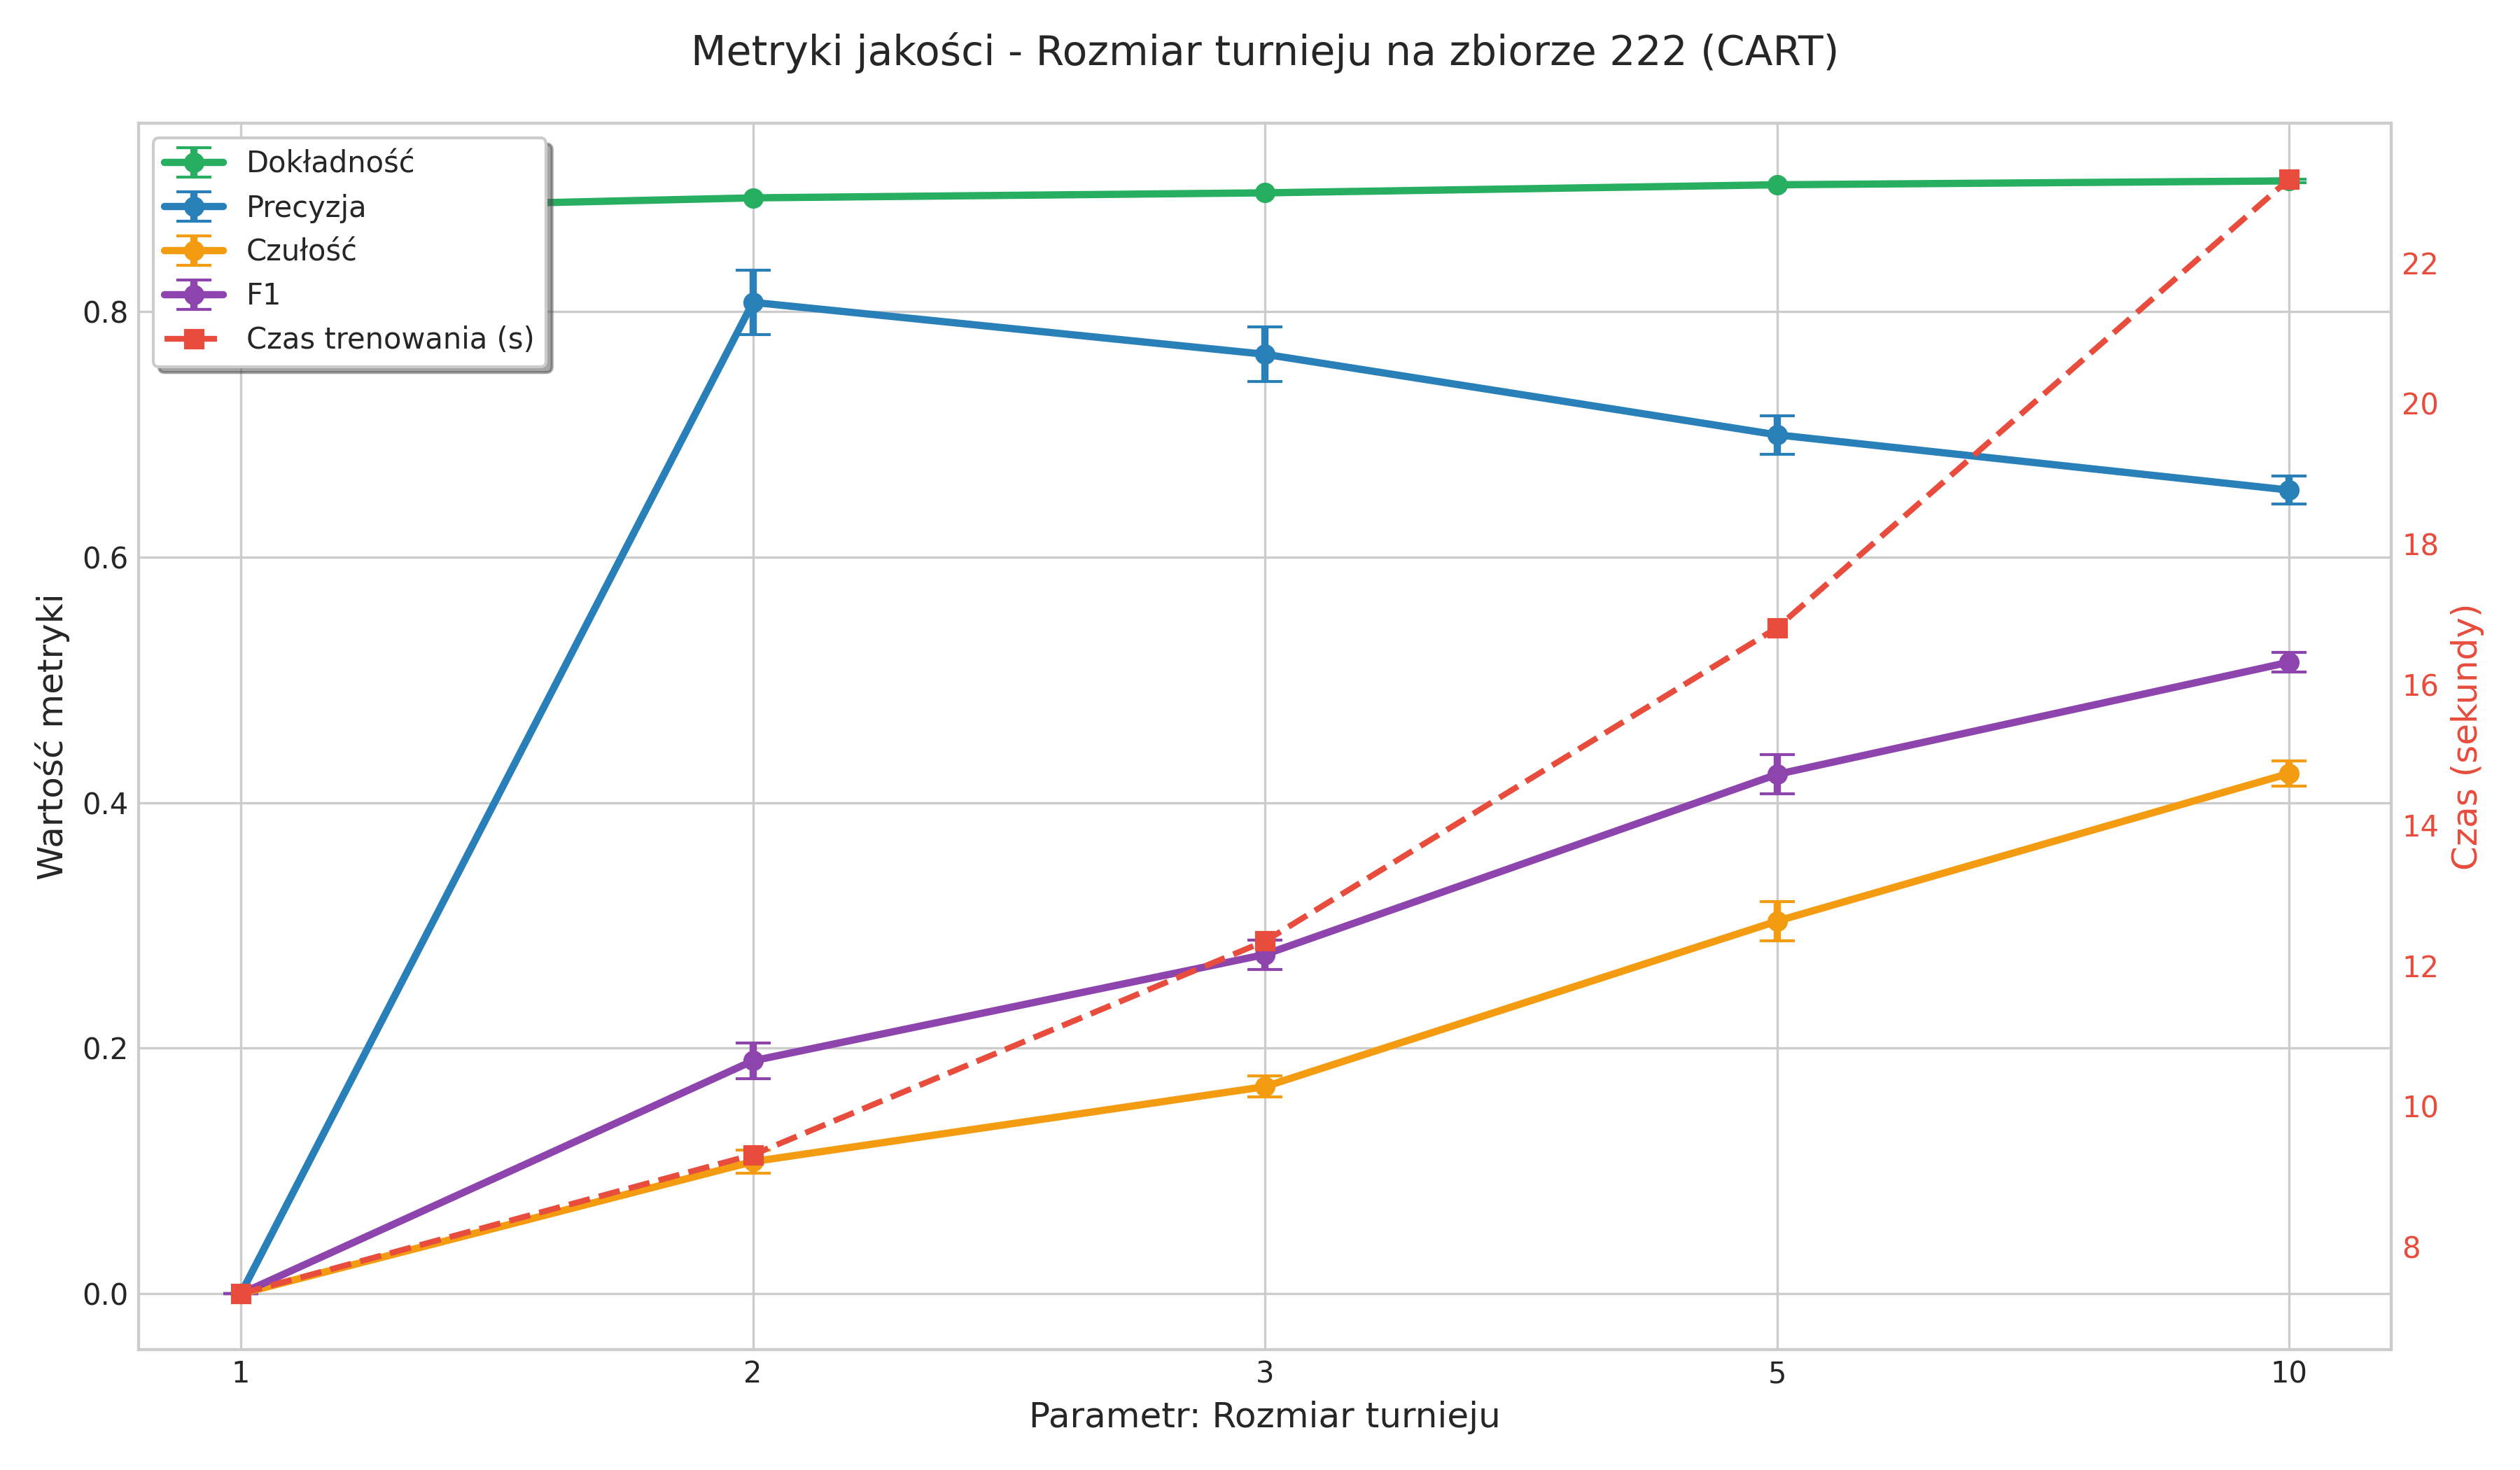
\includegraphics[width=0.9\textwidth]{plots/CART_tournament_size_222_metrics.png}
        \caption{Wpływ rozmiaru turnieju na dokładność modelu CART dla zbioru 222 - Skuteczność marketingu bankowego.}
        \label{fig:cart_tournament_size_222}
    \end{figure}

    \item Zbiór 350 - Zaległości płatnicze klientów kart kredytowych

    Na tym zbiorze wzrost rozmiaru turnieju nie wpływa znacząco na wyniki modelu.

    \begin{figure}[H]
        \centering
        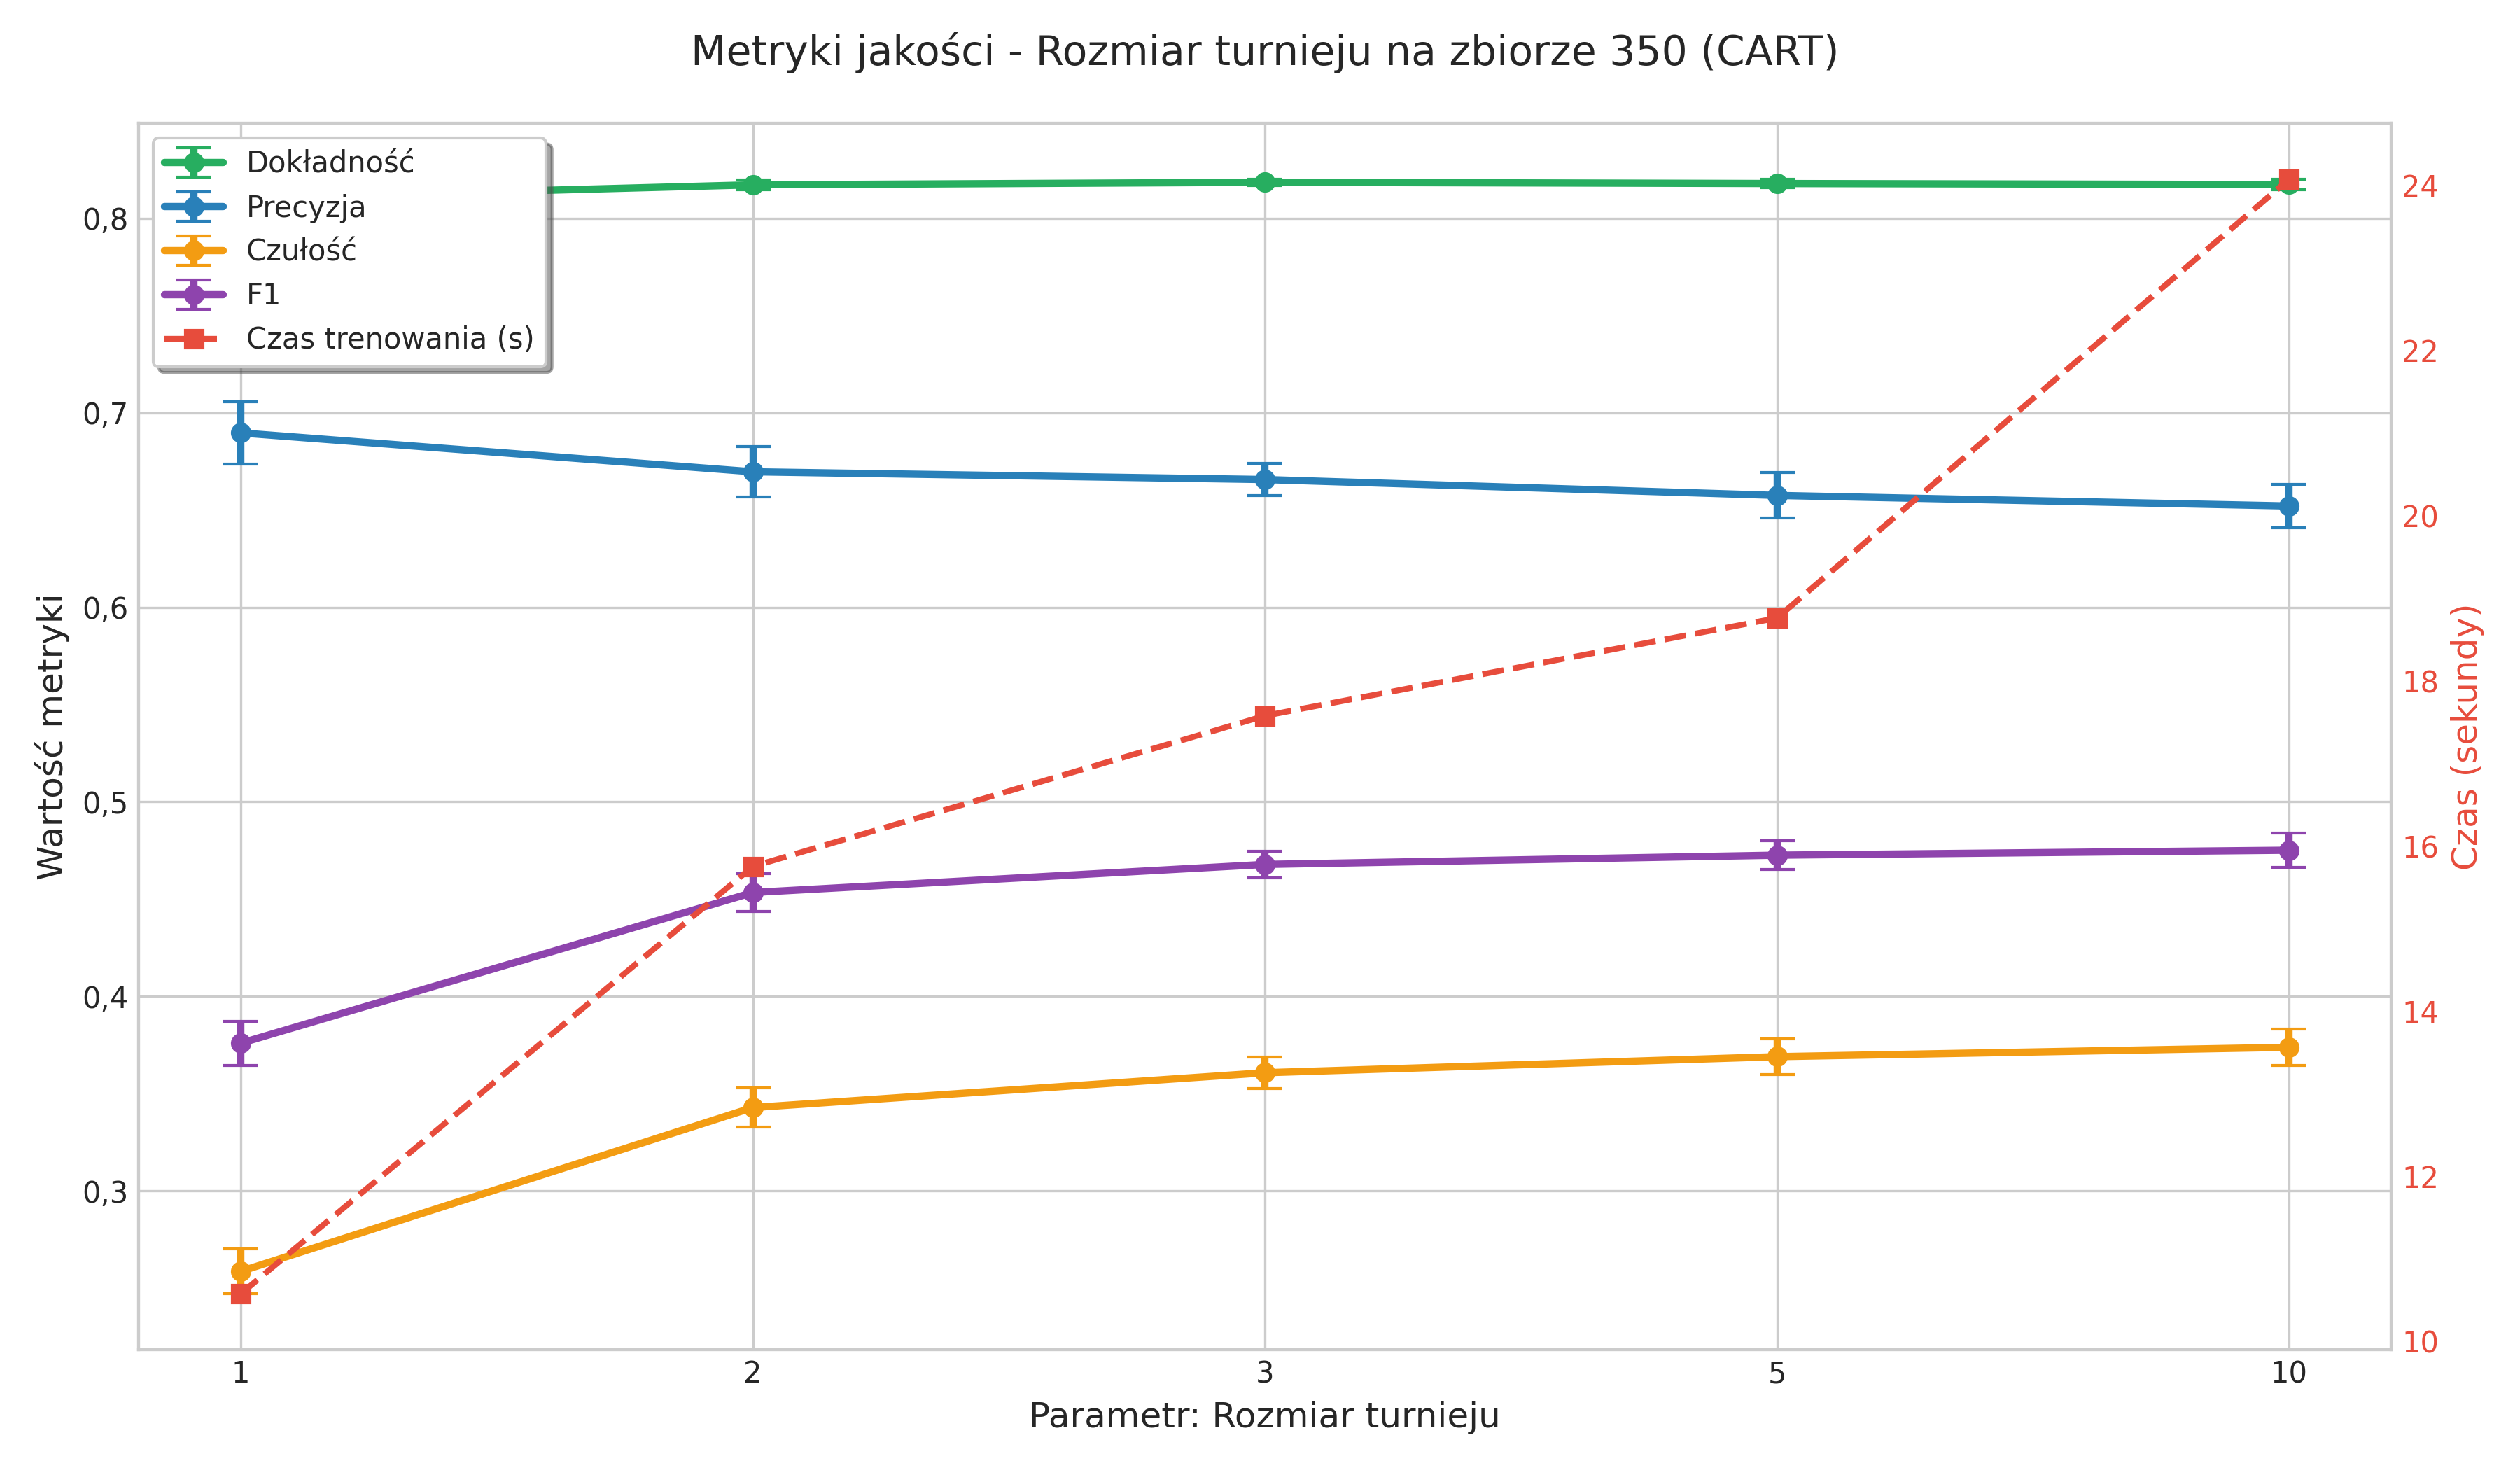
\includegraphics[width=0.9\textwidth]{plots/CART_tournament_size_350_metrics.png}
        \caption{Wpływ rozmiaru turnieju na dokładność modelu CART dla zbioru 350 - Zaległości płatnicze klientów kart kredytowych.}
        \label{fig:cart_tournament_size_350}
    \end{figure}
\end{itemize}

\subsubsection{Wnioski ogólne}
\begin{itemize}
    \item Wzrost liczebności turnieju zazwyczaj nie wpływa znacząco na dokładność modelu.
    \item Prowadzi jednak do zwiększenia zdolności wykrywania przez model klas mniejszościowych - zwiększenia czułości kosztem precyzji.
    \item Cecha ta może być użyteczna w przypadku zbiorów z niezbalansowanymi klasami w szczególności w pewnych rzeczywistych zastosowaniach,
    na przykład w medycynie, gdzie wykrycie choroby (klasa mniejszościowa) jest ważniejsze niż uniknięcie fałszywych alarmów.
    \item W porównaniu algorytmów zostanie przyjęty rozmiar turnieju równy 3 jako kompromis pomiędzy czułością a precyzją.
\end{itemize}

\subsection{Funkcja jakości  testu (tylko ID3)}

Dla drzew CART została zaimplementowana tylko jedna taka funkcja, dlatego badanie nie zostało wykonane.

\begin{itemize}
    \item Zbiór 73 - Grzyby

    Zastosowana funkcja miary jakości nie ma żadnego wpływu na wyniki modelu na tym trywialnym zbiorze danych.

    \begin{figure}[H]
        \centering
        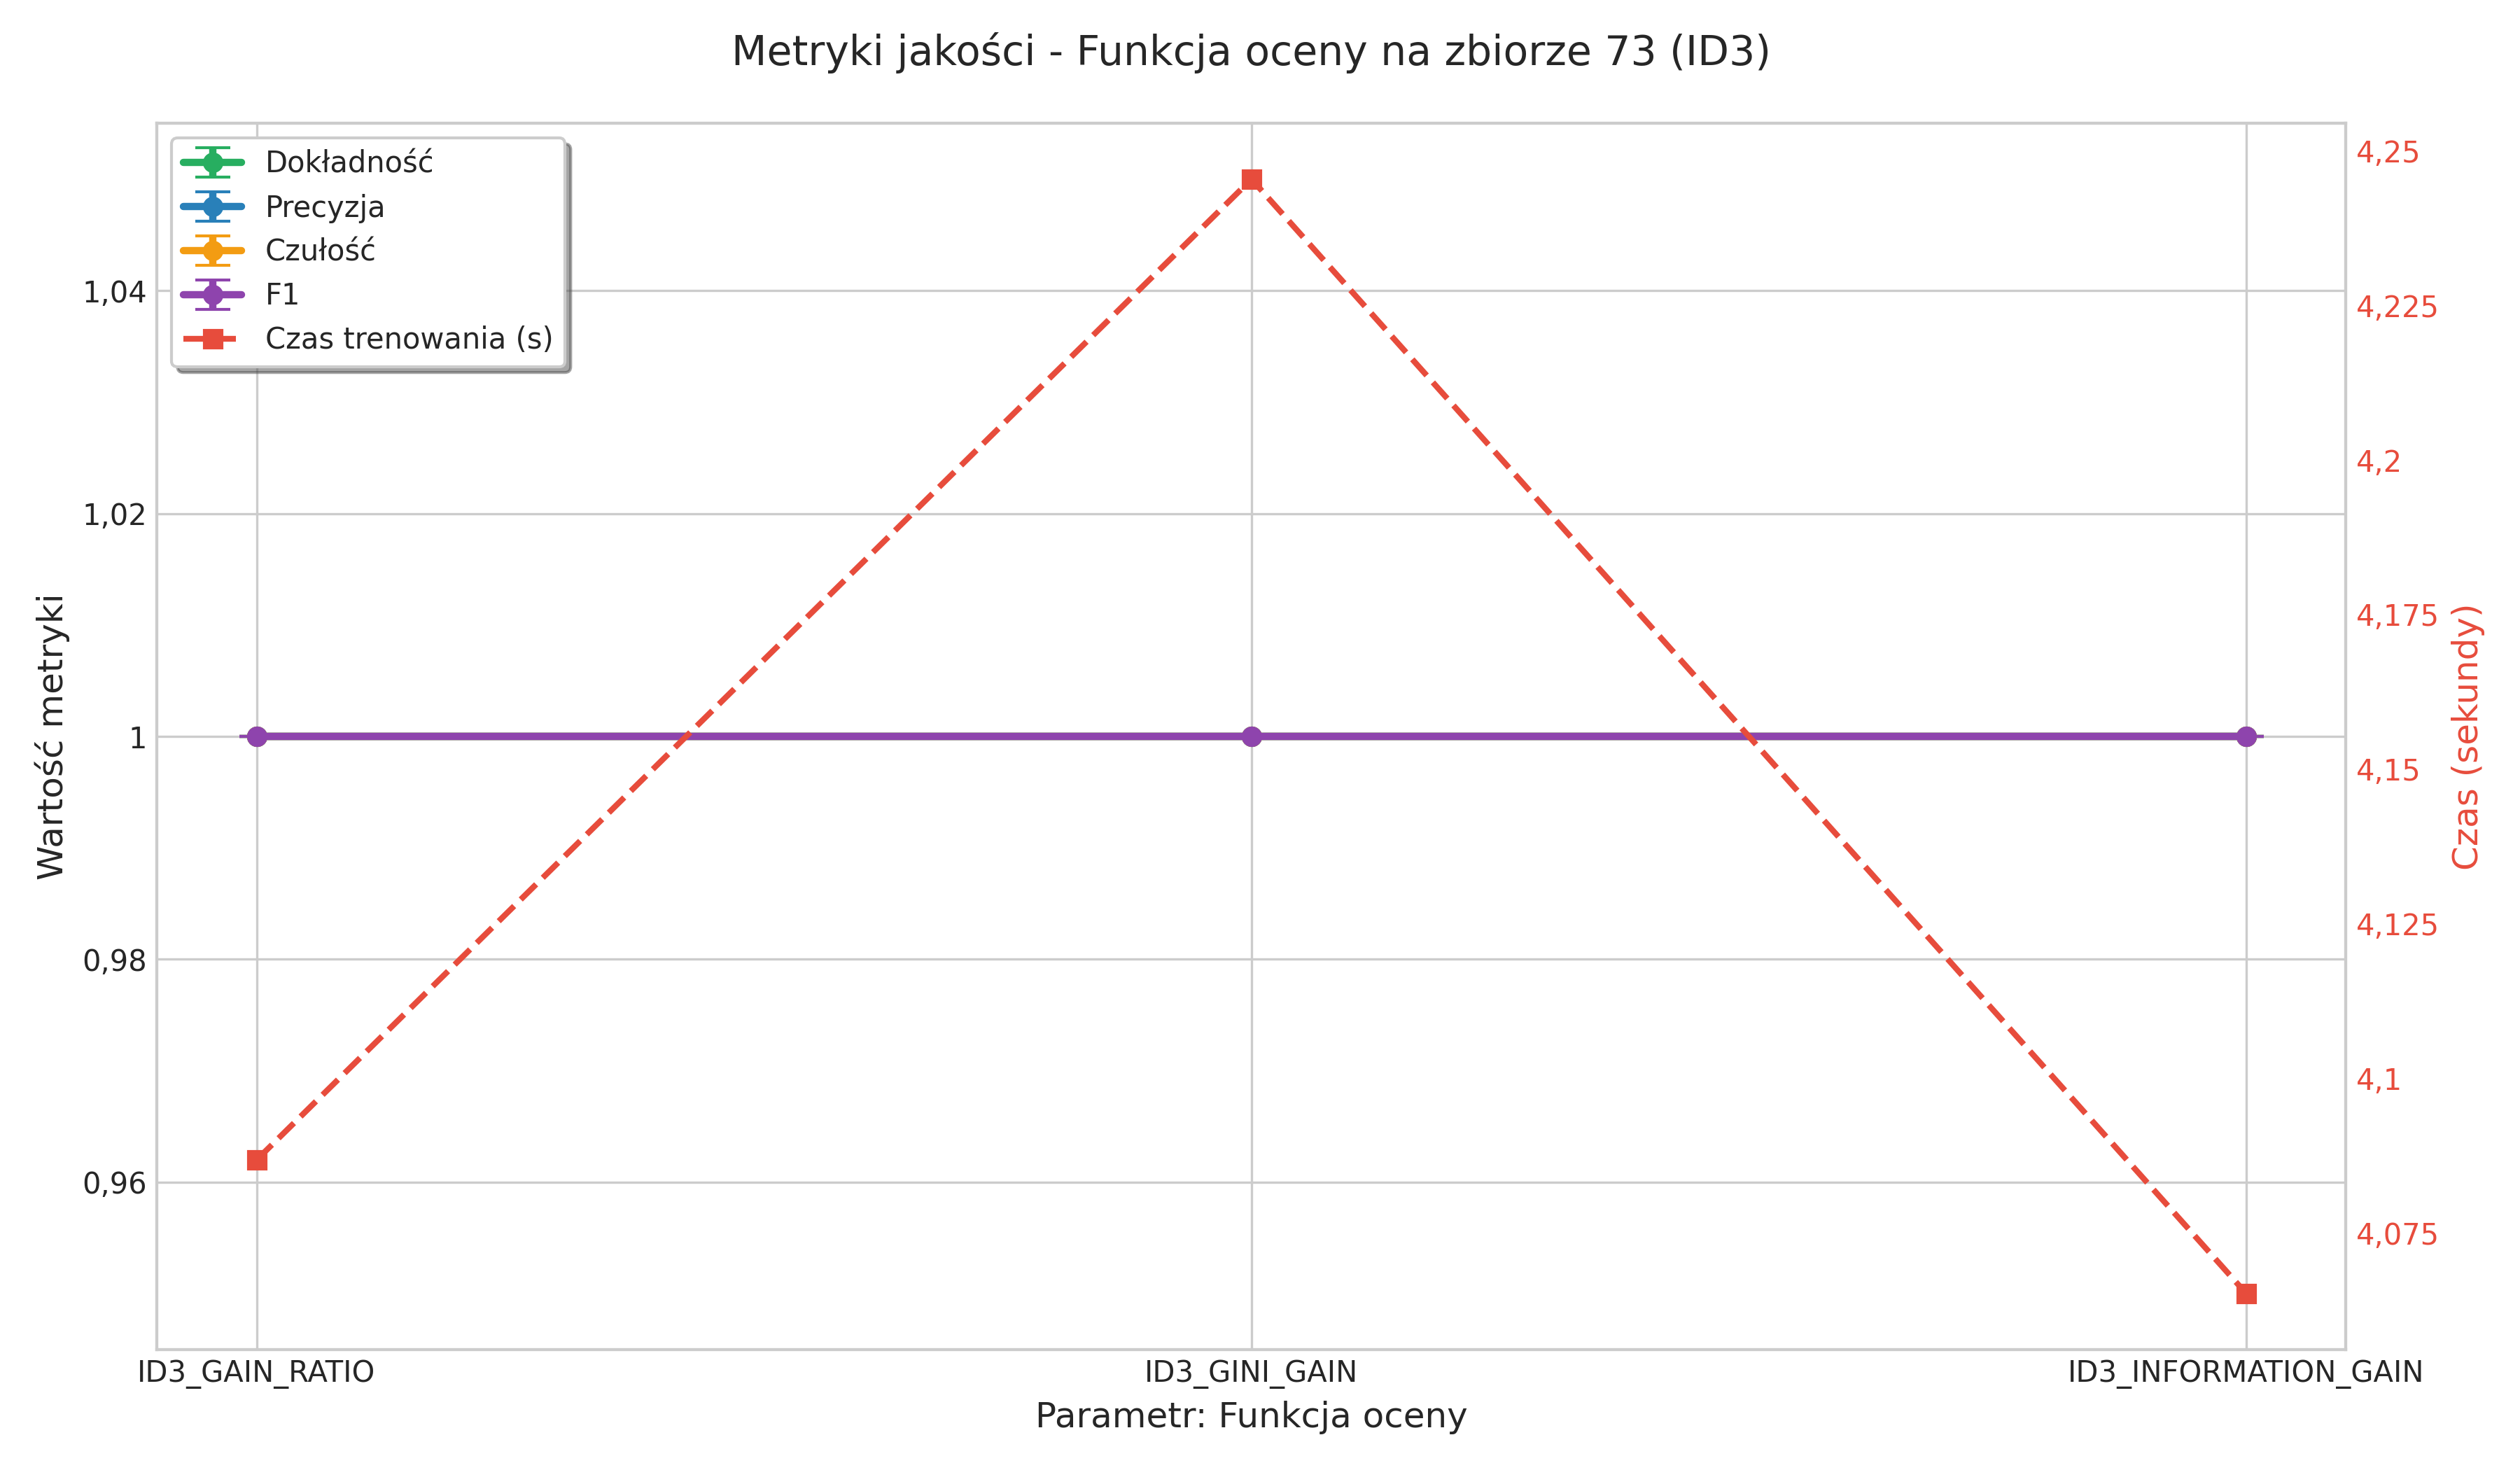
\includegraphics[width=0.9\textwidth]{plots/ID3_eval_function_73_metrics.png}
        \caption{Wpływ funkcji jakości testu na dokładność modelu ID3 dla zbioru 73 - Grzyby.}
        \label{fig:id3_eval_function_73}
    \end{figure}

    \item Zbiór 14 - Nawrót raka piersi

    Delikatnie wyróżniła się funkcja \textbf{gain ratio}, dla której wszystkie miary są minimalnie większe. Różnica jest na tyle mała, że może
    być to uznane za szum statystyczny, jednak z uwagi na brak innych przesłanek zostanie ona wybrana jako domyślna dla drzew ID3 w porównaniu modeli.

    \begin{figure}[H]
        \centering
        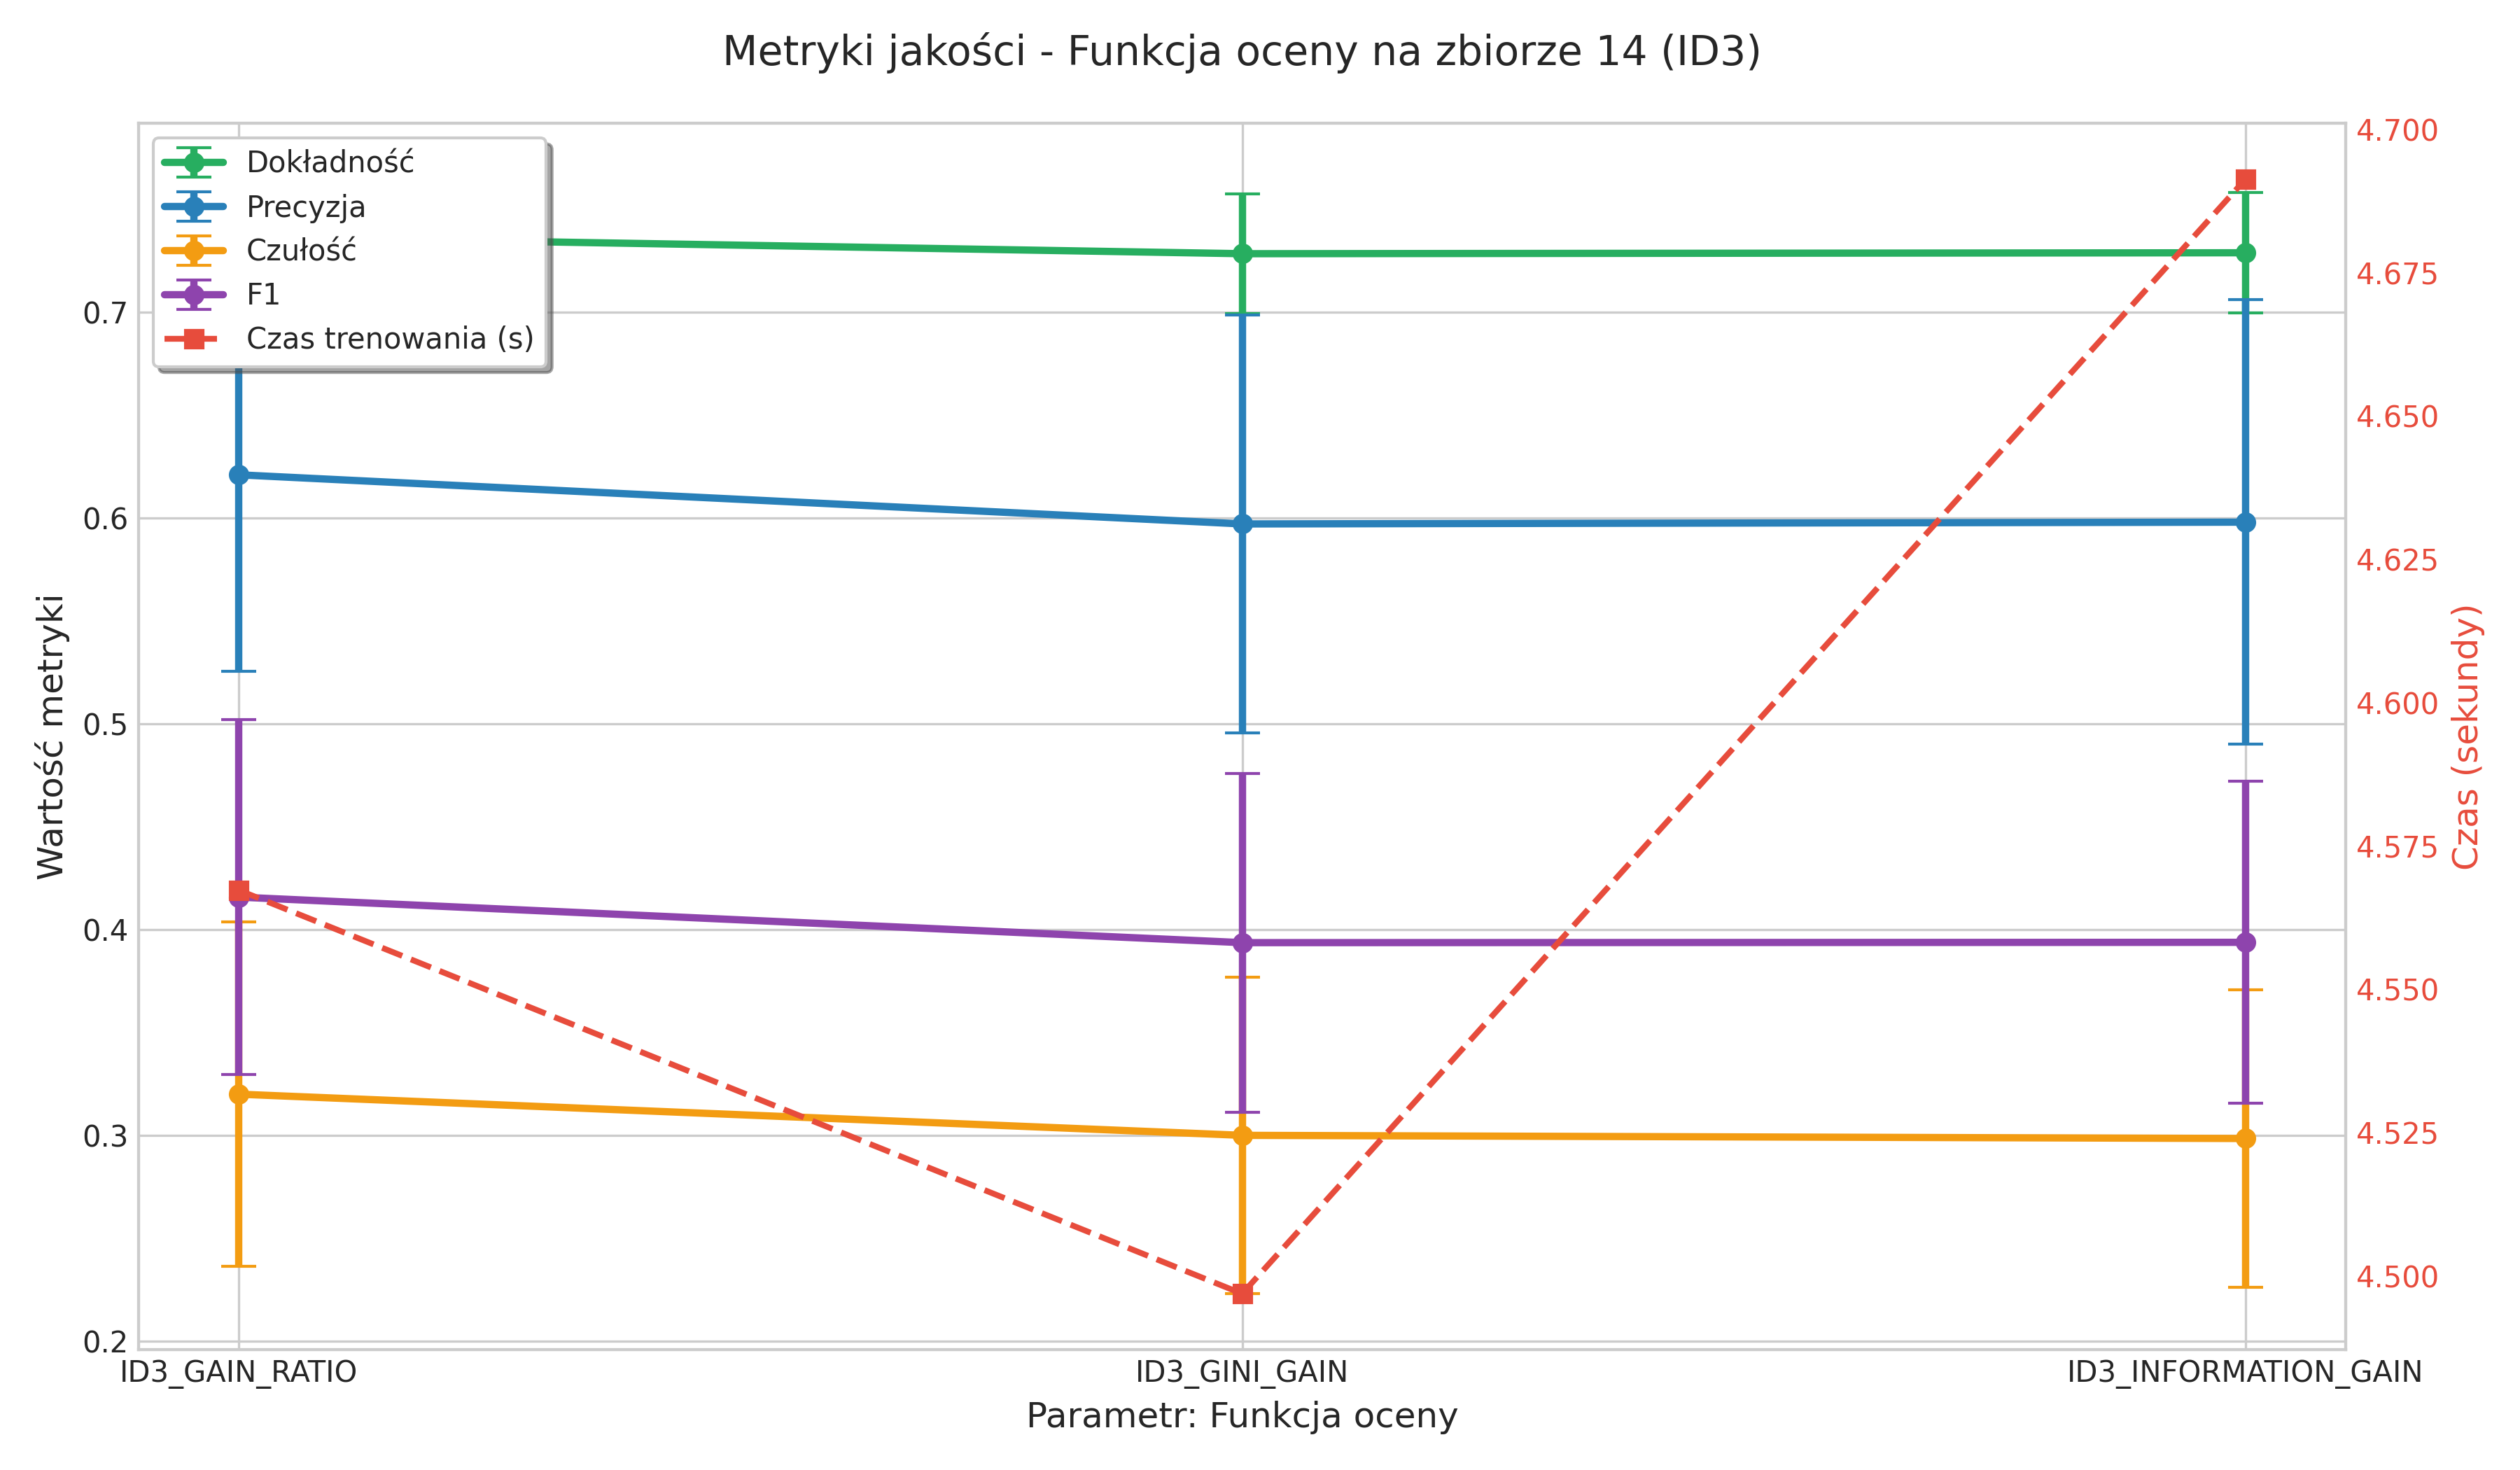
\includegraphics[width=0.9\textwidth]{plots/ID3_eval_function_14_metrics.png}
        \caption{Wpływ funkcji jakości testu na dokładność modelu ID3 dla zbioru 14 - Nawrót raka piersi.}
        \label{fig:id3_eval_function_14}
    \end{figure}

\end{itemize}

\section{Porównanie modeli}

Przyjęte hiperparametry zostały skorygowane o wyniki z poprzedniego punktu badań - zmienił się jedynie rozmiar turnieju na 3.
W porównaniu pominięty został trywialny zbiór grzybów. Drzewo ID3 było porównywane jedynie na zbiorze nawrotu raka piersi.
Lasy ID3 oraz CART stanowią naszą własną implementację z wyborem atrybutów podziału na podstawie turnieju, natomiast
las SKLEARN to standardowy, niezmodyfikowany las losowy.

\subsection{Zbiór 14 - Nawrót raka piersi}

    \begin{figure}[H]
        \centering
        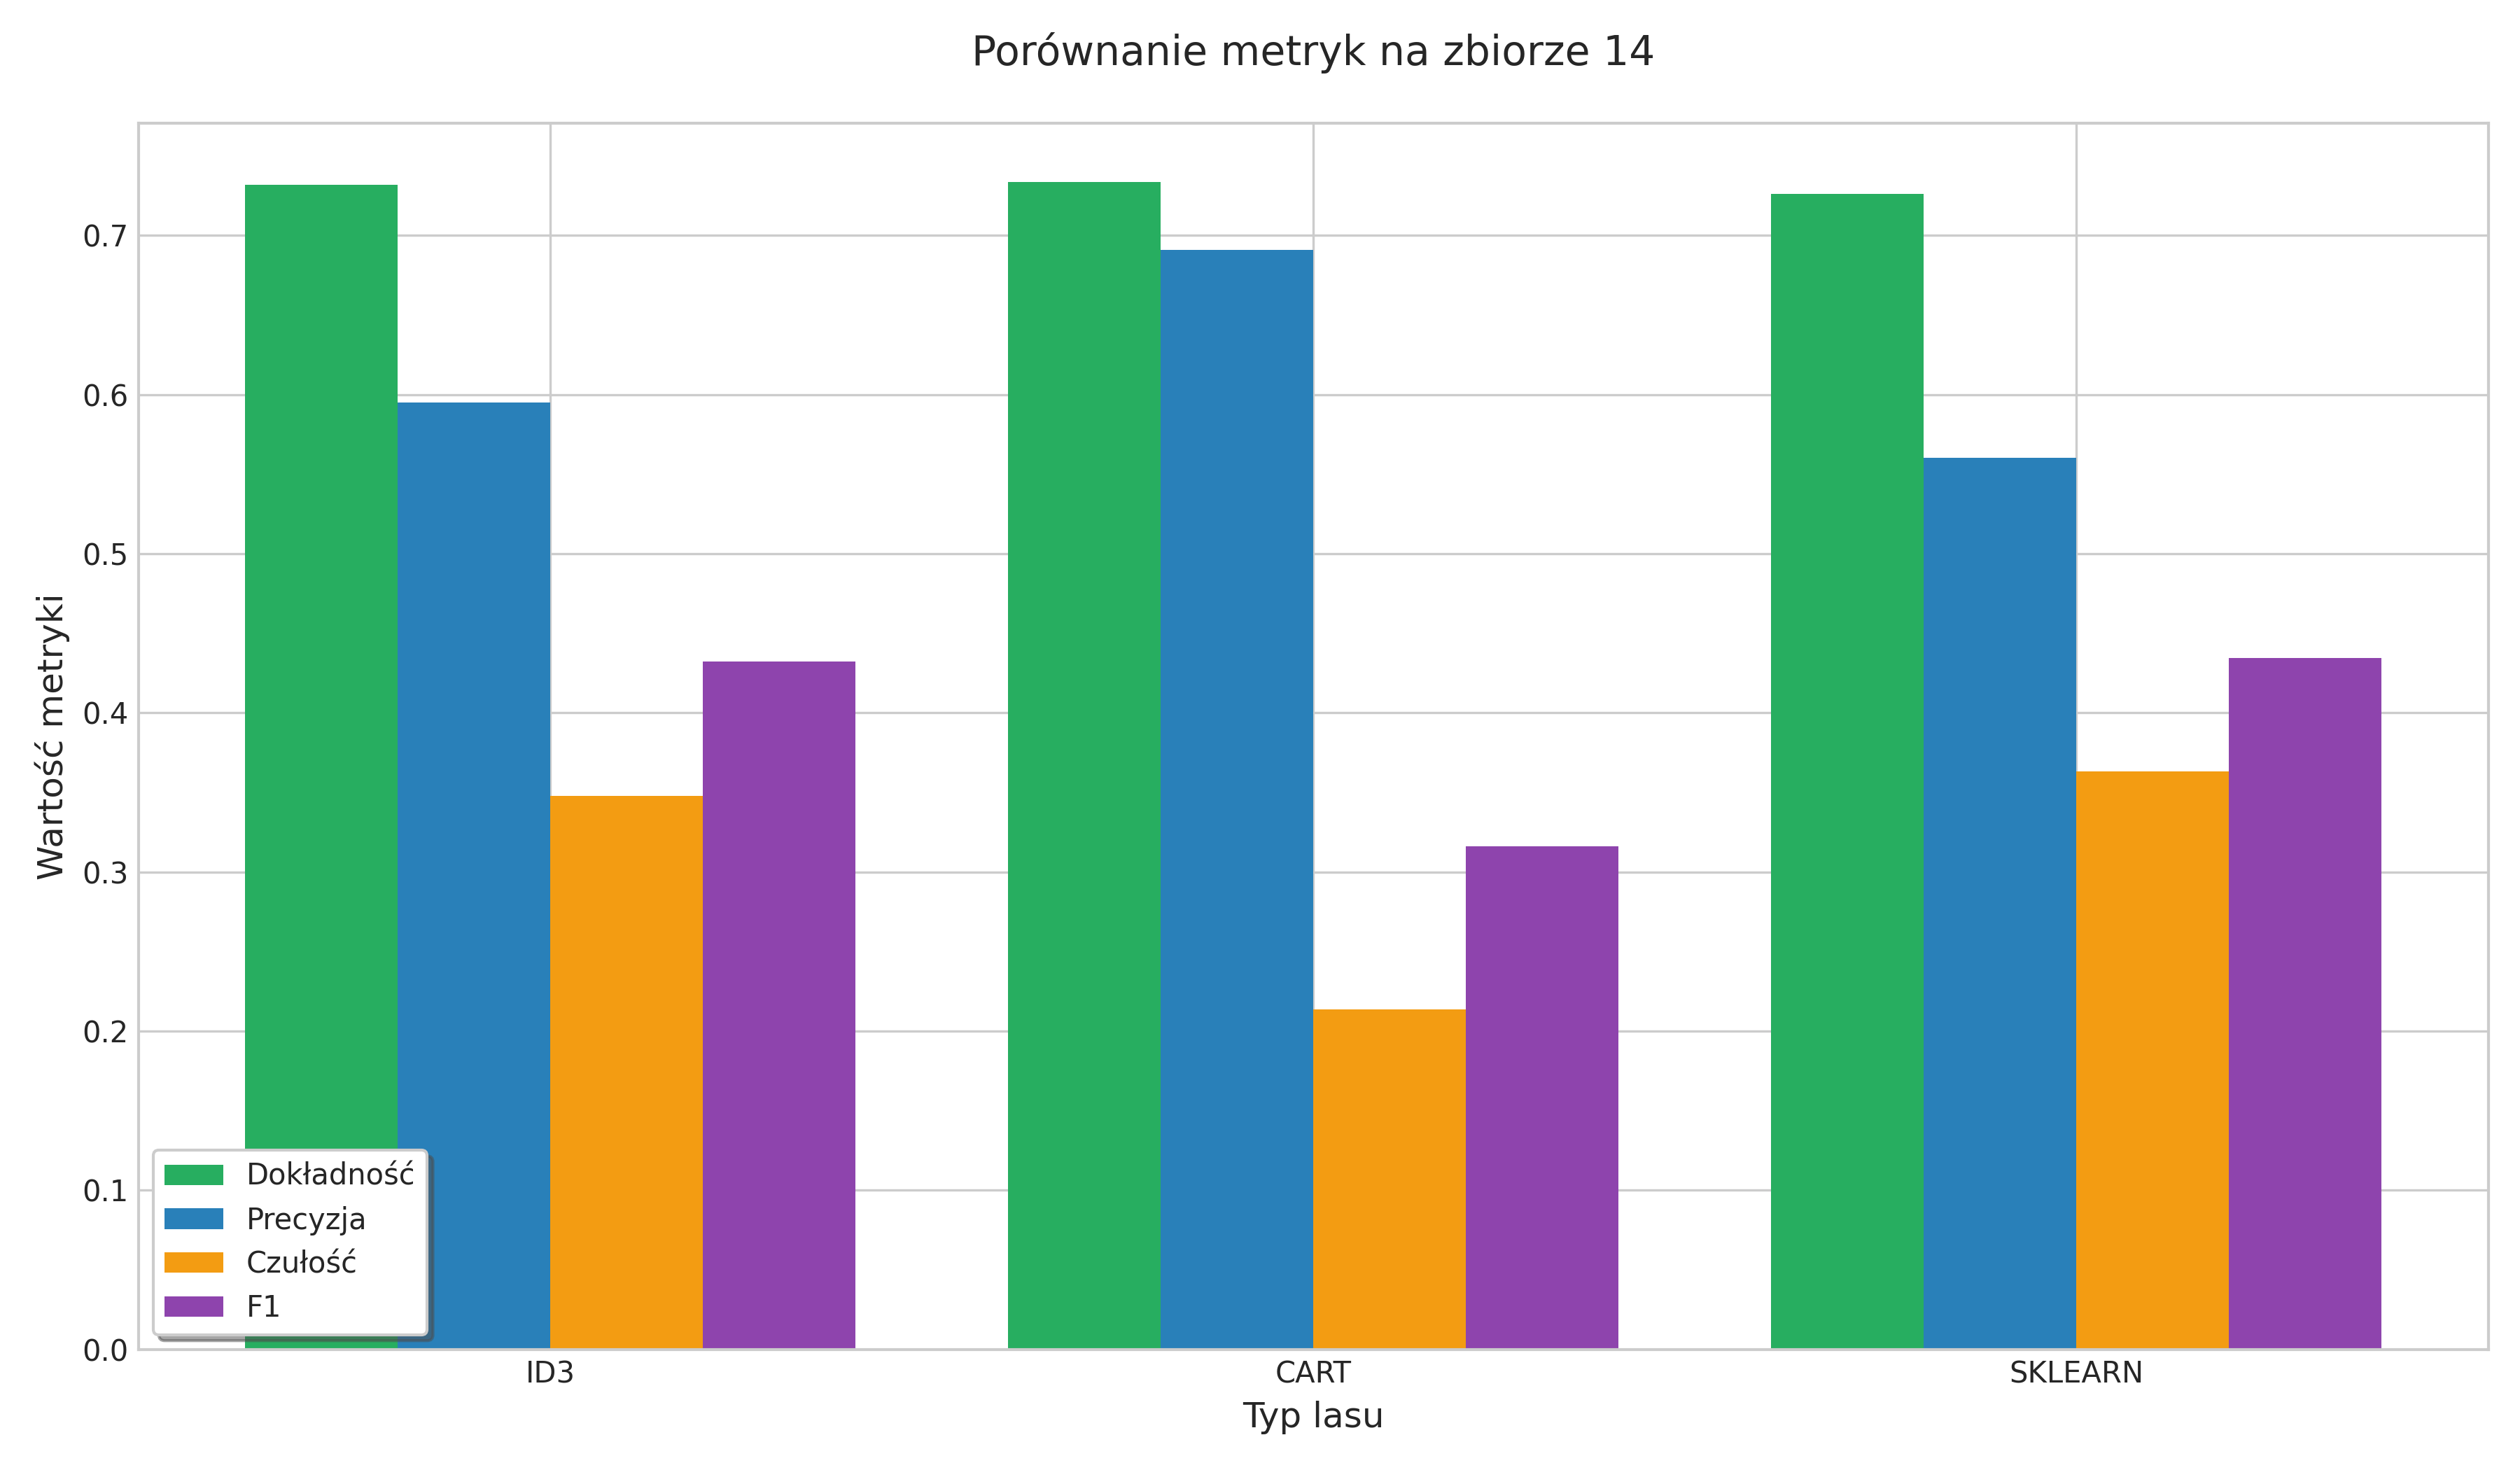
\includegraphics[width=0.9\textwidth]{plots/Compare_on_14_compare_metrics.png}
        \caption{Porównanie modeli dla zbioru 14 - Nawrót raka piersi.}
        \label{fig:compare_on_14}
    \end{figure}

    \begin{table}[htbp]
        \centering
        \small
        \setlength{\tabcolsep}{4pt}
        \renewcommand{\arraystretch}{1.2}

        \begin{minipage}[t]{0.48\textwidth}
            \centering
            \caption{\textbf{Dokładność} - Typ lasu (zbiór 14)}
            \label{tab:Compare_on_14_acc}
            \begin{tabular}{r|r|r|r|r}
                \toprule
                Typ lasu & Średnia & Std & Maks & Min \\
                \hline
                \textbf{CART} & \textbf{0,734} & \textbf{0,021} & \textbf{0,793} & \textbf{0,701} \\
                ID3 & 0,732 & 0,026 & 0,770 & 0,667 \\
                SKLEARN & 0,726 & 0,028 & 0,782 & 0,678 \\
                \bottomrule
            \end{tabular}
        \end{minipage}
        \hfill
        \begin{minipage}[t]{0.48\textwidth}
            \centering
            \caption{\textbf{Precyzja} - Typ lasu (zbiór 14)}
            \label{tab:Compare_on_14_prec}
            \begin{tabular}{r|r|r|r|r}
                \toprule
                Typ lasu & Średnia & Std & Maks & Min \\
                \hline
                \textbf{CART} & \textbf{0,691} & \textbf{0,132} & \textbf{1,000} & \textbf{0,500} \\
                ID3 & 0,595 & 0,081 & 0,727 & 0,412 \\
                SKLEARN & 0,561 & 0,070 & 0,667 & 0,429 \\
                \bottomrule
            \end{tabular}
        \end{minipage}

        \vspace{0.5cm}

        \begin{minipage}[t]{0.48\textwidth}
            \centering
            \caption{\textbf{Czułość} - Typ lasu (zbiór 14)}
            \label{tab:Compare_on_14_rec}
            \begin{tabular}{r|r|r|r|r}
                \toprule
                Typ lasu & Średnia & Std & Maks & Min \\
                \hline
                CART & 0,214 & 0,084 & 0,423 & 0,077 \\
                ID3 & 0,348 & 0,080 & 0,462 & 0,154 \\
                \textbf{SKLEARN} & \textbf{0,363} & \textbf{0,108} & \textbf{0,577} & \textbf{0,115} \\
                \bottomrule
            \end{tabular}
        \end{minipage}
        \hfill
        \begin{minipage}[t]{0.48\textwidth}
            \centering
            \caption{\textbf{F1} - Typ lasu (zbiór 14)}
            \label{tab:Compare_on_14_f1}
            \begin{tabular}{r|r|r|r|r}
                \toprule
                Typ lasu & Średnia & Std & Maks & Min \\
                \hline
                CART & 0,316 & 0,099 & 0,550 & 0,138 \\
                ID3 & 0,432 & 0,075 & 0,545 & 0,250 \\
                \textbf{SKLEARN} & \textbf{0,434} & \textbf{0,096} & \textbf{0,612} & \textbf{0,188} \\
                \bottomrule
            \end{tabular}
        \end{minipage}
    \end{table}

    CART oraz ID3 nieznacznie przewyższają implementację z biblioteki SKLEARN pod względem dokładności. Lepszymi właściwościami charakteryzuje się
    tutaj las ID3, który stanowi lepszy balans pomiędzy precyzją a czułością, co przekłada się na wyższe wartości F1-score.
    Na tym zbiorze skorzystanie z wyboru atrybutów podziału węzła na podstawie turnieju okazało się korzystne.

\subsection{Zbiór 222 - Skuteczność marketingu bankowego}

    \begin{figure}[H]
        \centering
        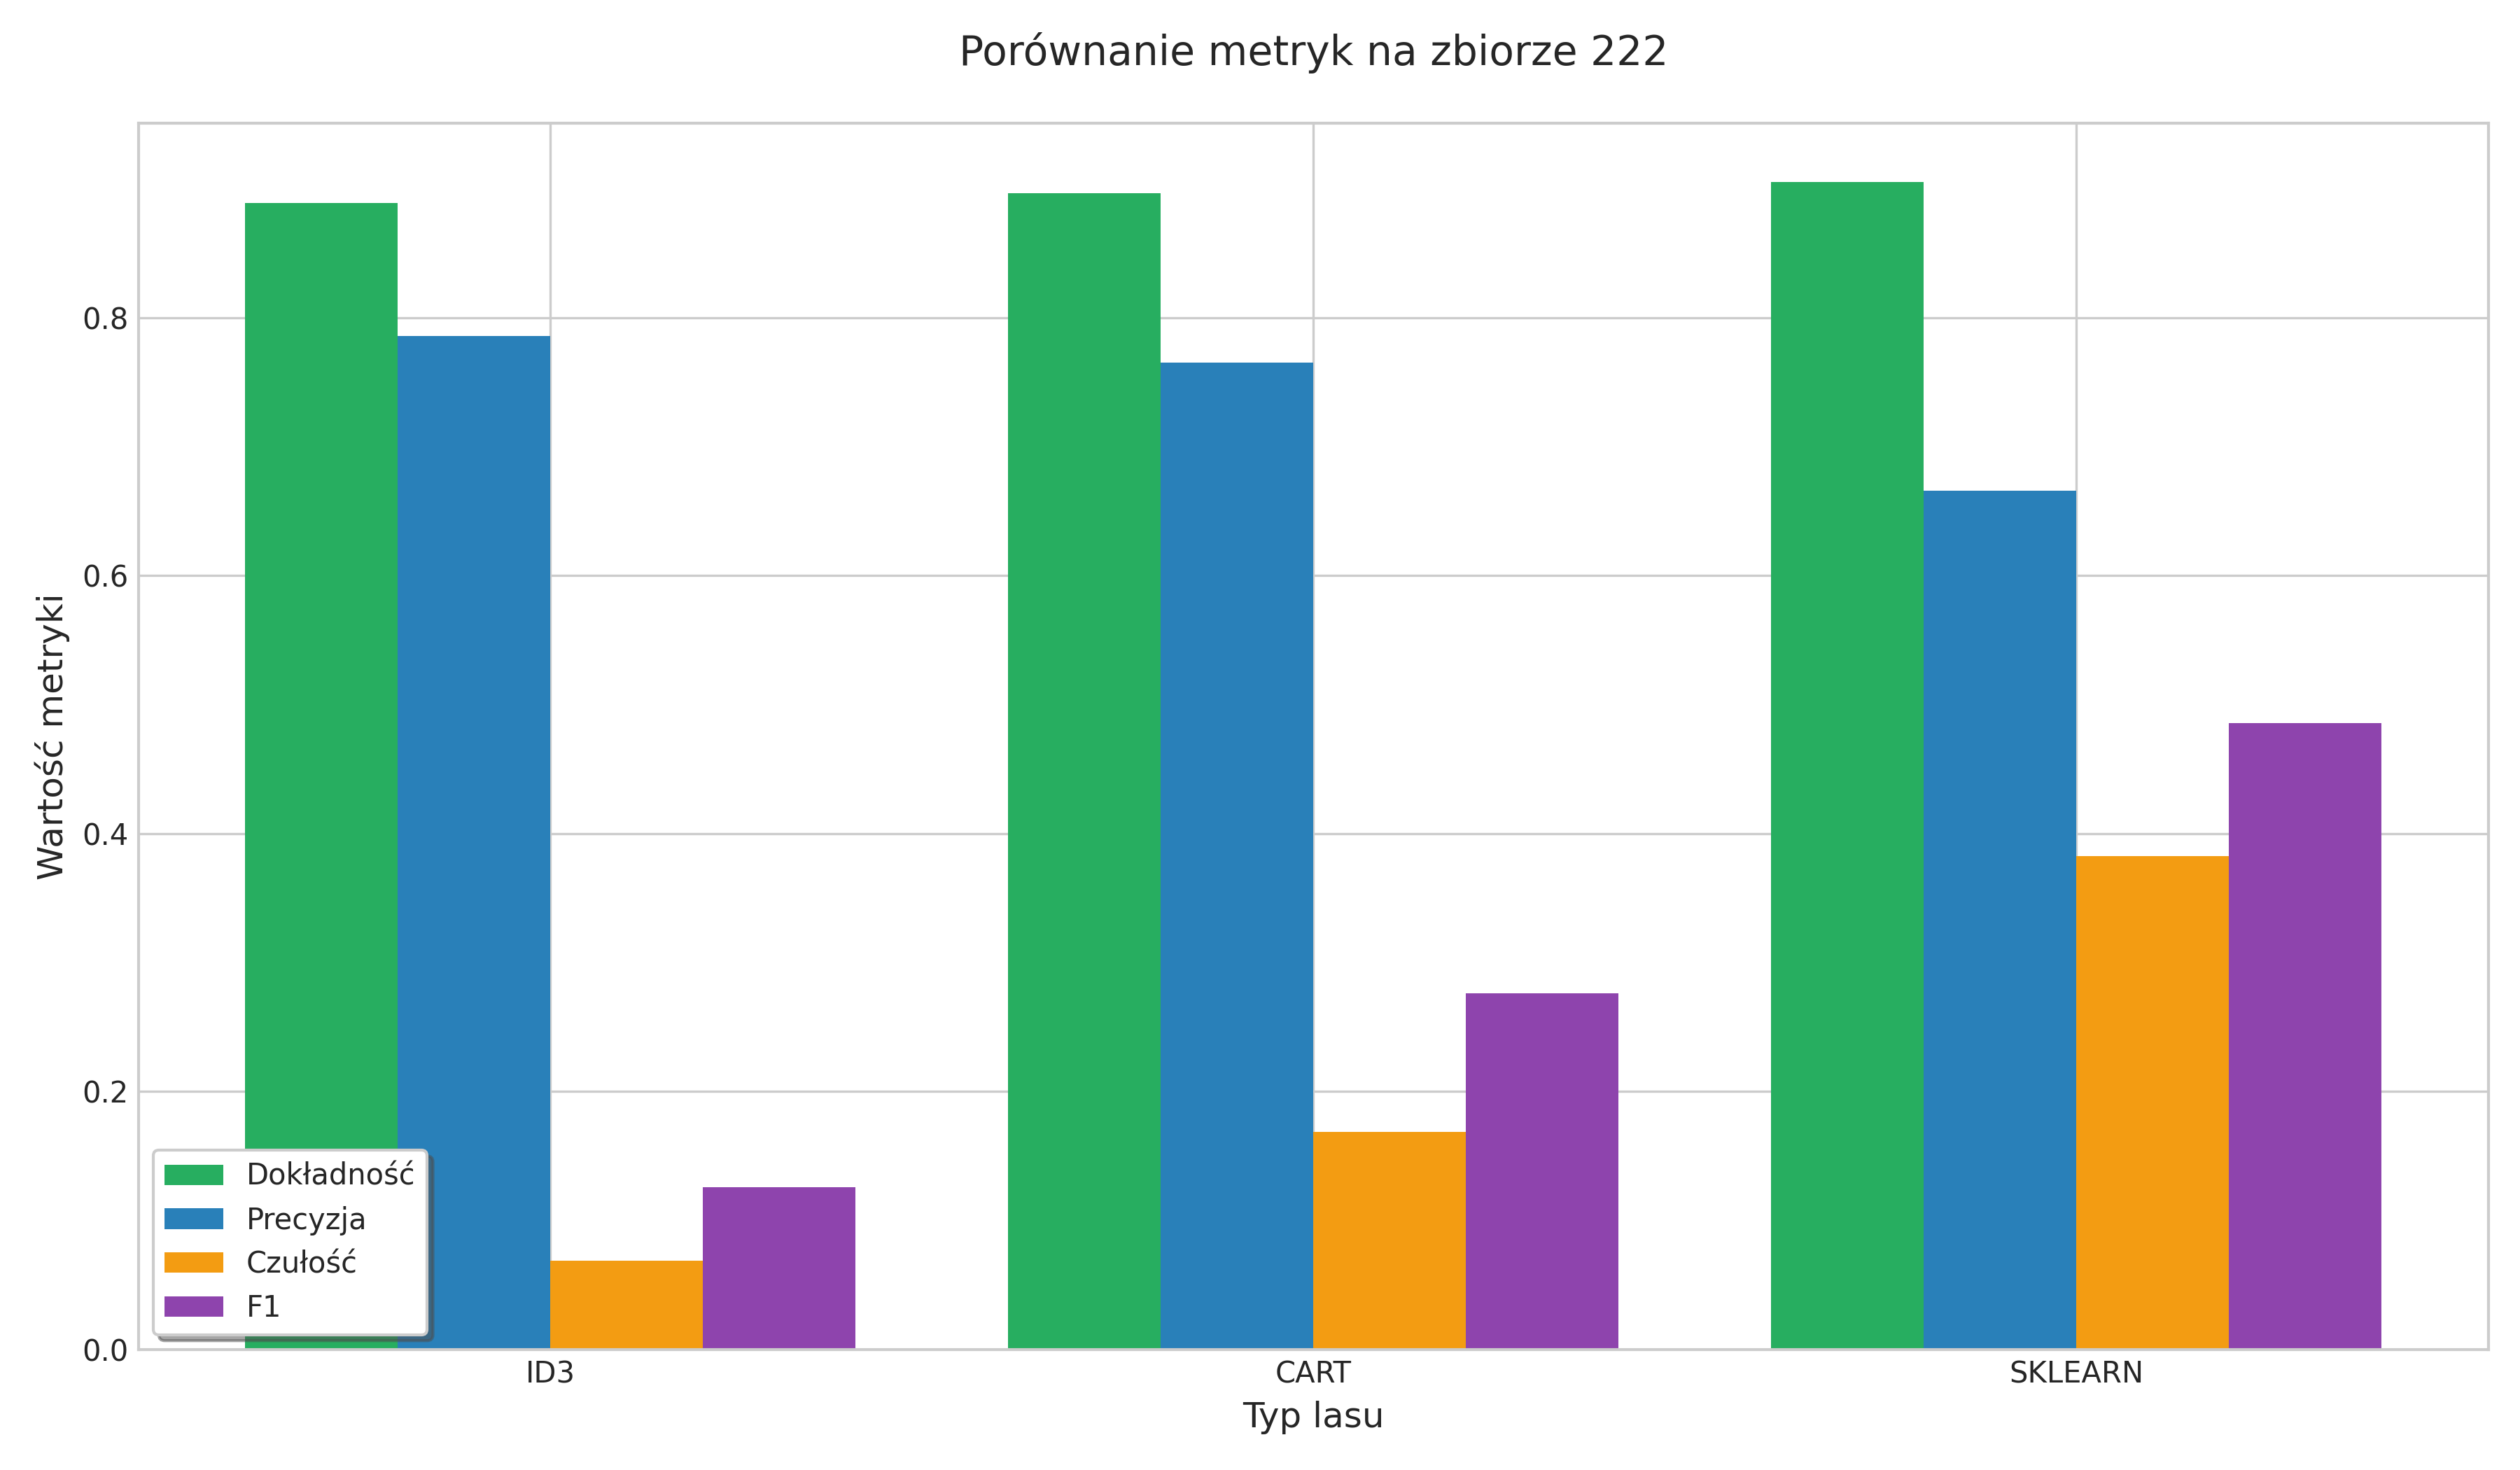
\includegraphics[width=0.9\textwidth]{plots/Compare_on_222_compare_metrics.png}
        \caption{Porównanie modeli dla zbioru 222 - Skuteczność marketingu bankowego.}
        \label{fig:compare_on_222}
    \end{figure}

    \begin{table}[htbp]
        \centering
        \small
        \setlength{\tabcolsep}{4pt}
        \renewcommand{\arraystretch}{1.2}

        \begin{minipage}[t]{0.48\textwidth}
            \centering
            \caption{\textbf{Dokładność} - Typ lasu (zbiór 222)}
            \label{tab:Compare_on_222_acc}
            \begin{tabular}{r|r|r|r|r}
                \toprule
                Typ lasu & Średnia & Std & Maks & Min \\
                \hline
                CART & 0,897 & 0,001 & 0,899 & 0,894 \\
                \textbf{SKLEARN} & \textbf{0,905} & \textbf{0,002} & \textbf{0,909} & \textbf{0,901} \\
                \bottomrule
            \end{tabular}
        \end{minipage}
        \hfill
        \begin{minipage}[t]{0.48\textwidth}
            \centering
            \caption{\textbf{Precyzja} - Typ lasu (zbiór 222)}
            \label{tab:Compare_on_222_prec}
            \begin{tabular}{r|r|r|r|r}
                \toprule
                Typ lasu & Średnia & Std & Maks & Min \\
                \hline
                \textbf{CART} & \textbf{0,765} & \textbf{0,022} & \textbf{0,805} & \textbf{0,704} \\
                SKLEARN & 0,666 & 0,013 & 0,689 & 0,634 \\
                \bottomrule
            \end{tabular}
        \end{minipage}

        \vspace{0.5cm}

        \begin{minipage}[t]{0.48\textwidth}
            \centering
            \caption{\textbf{Czułość} - Typ lasu (zbiór 222)}
            \label{tab:Compare_on_222_rec}
            \begin{tabular}{r|r|r|r|r}
                \toprule
                Typ lasu & Średnia & Std & Maks & Min \\
                \hline
                CART & 0,169 & 0,009 & 0,190 & 0,153 \\
                \textbf{SKLEARN} & \textbf{0,383} & \textbf{0,013} & \textbf{0,407} & \textbf{0,358} \\
                \bottomrule
            \end{tabular}
        \end{minipage}
        \hfill
        \begin{minipage}[t]{0.48\textwidth}
            \centering
            \caption{\textbf{F1} - Typ lasu (zbiór 222)}
            \label{tab:Compare_on_222_f1}
            \begin{tabular}{r|r|r|r|r}
                \toprule
                Typ lasu & Średnia & Std & Maks & Min \\
                \hline
                CART & 0,276 & 0,012 & 0,305 & 0,255 \\
                \textbf{SKLEARN} & \textbf{0,486} & \textbf{0,012} & \textbf{0,511} & \textbf{0,458} \\
                \bottomrule
            \end{tabular}
        \end{minipage}
    \end{table}

    Implementacja lasu CART uzyskała nieco niższą dokładność niż las z biblioteki SKLEARN oraz cechuje się gorszymi właściwościami ogólnymi.
    Zastosowanie modyfikacji lasu nie jest w tym przypadku uzasadnione.

\subsection{Zbiór 350 - Zaległości płatnicze klientów kart kredytowych}

    \begin{figure}[H]
        \centering
        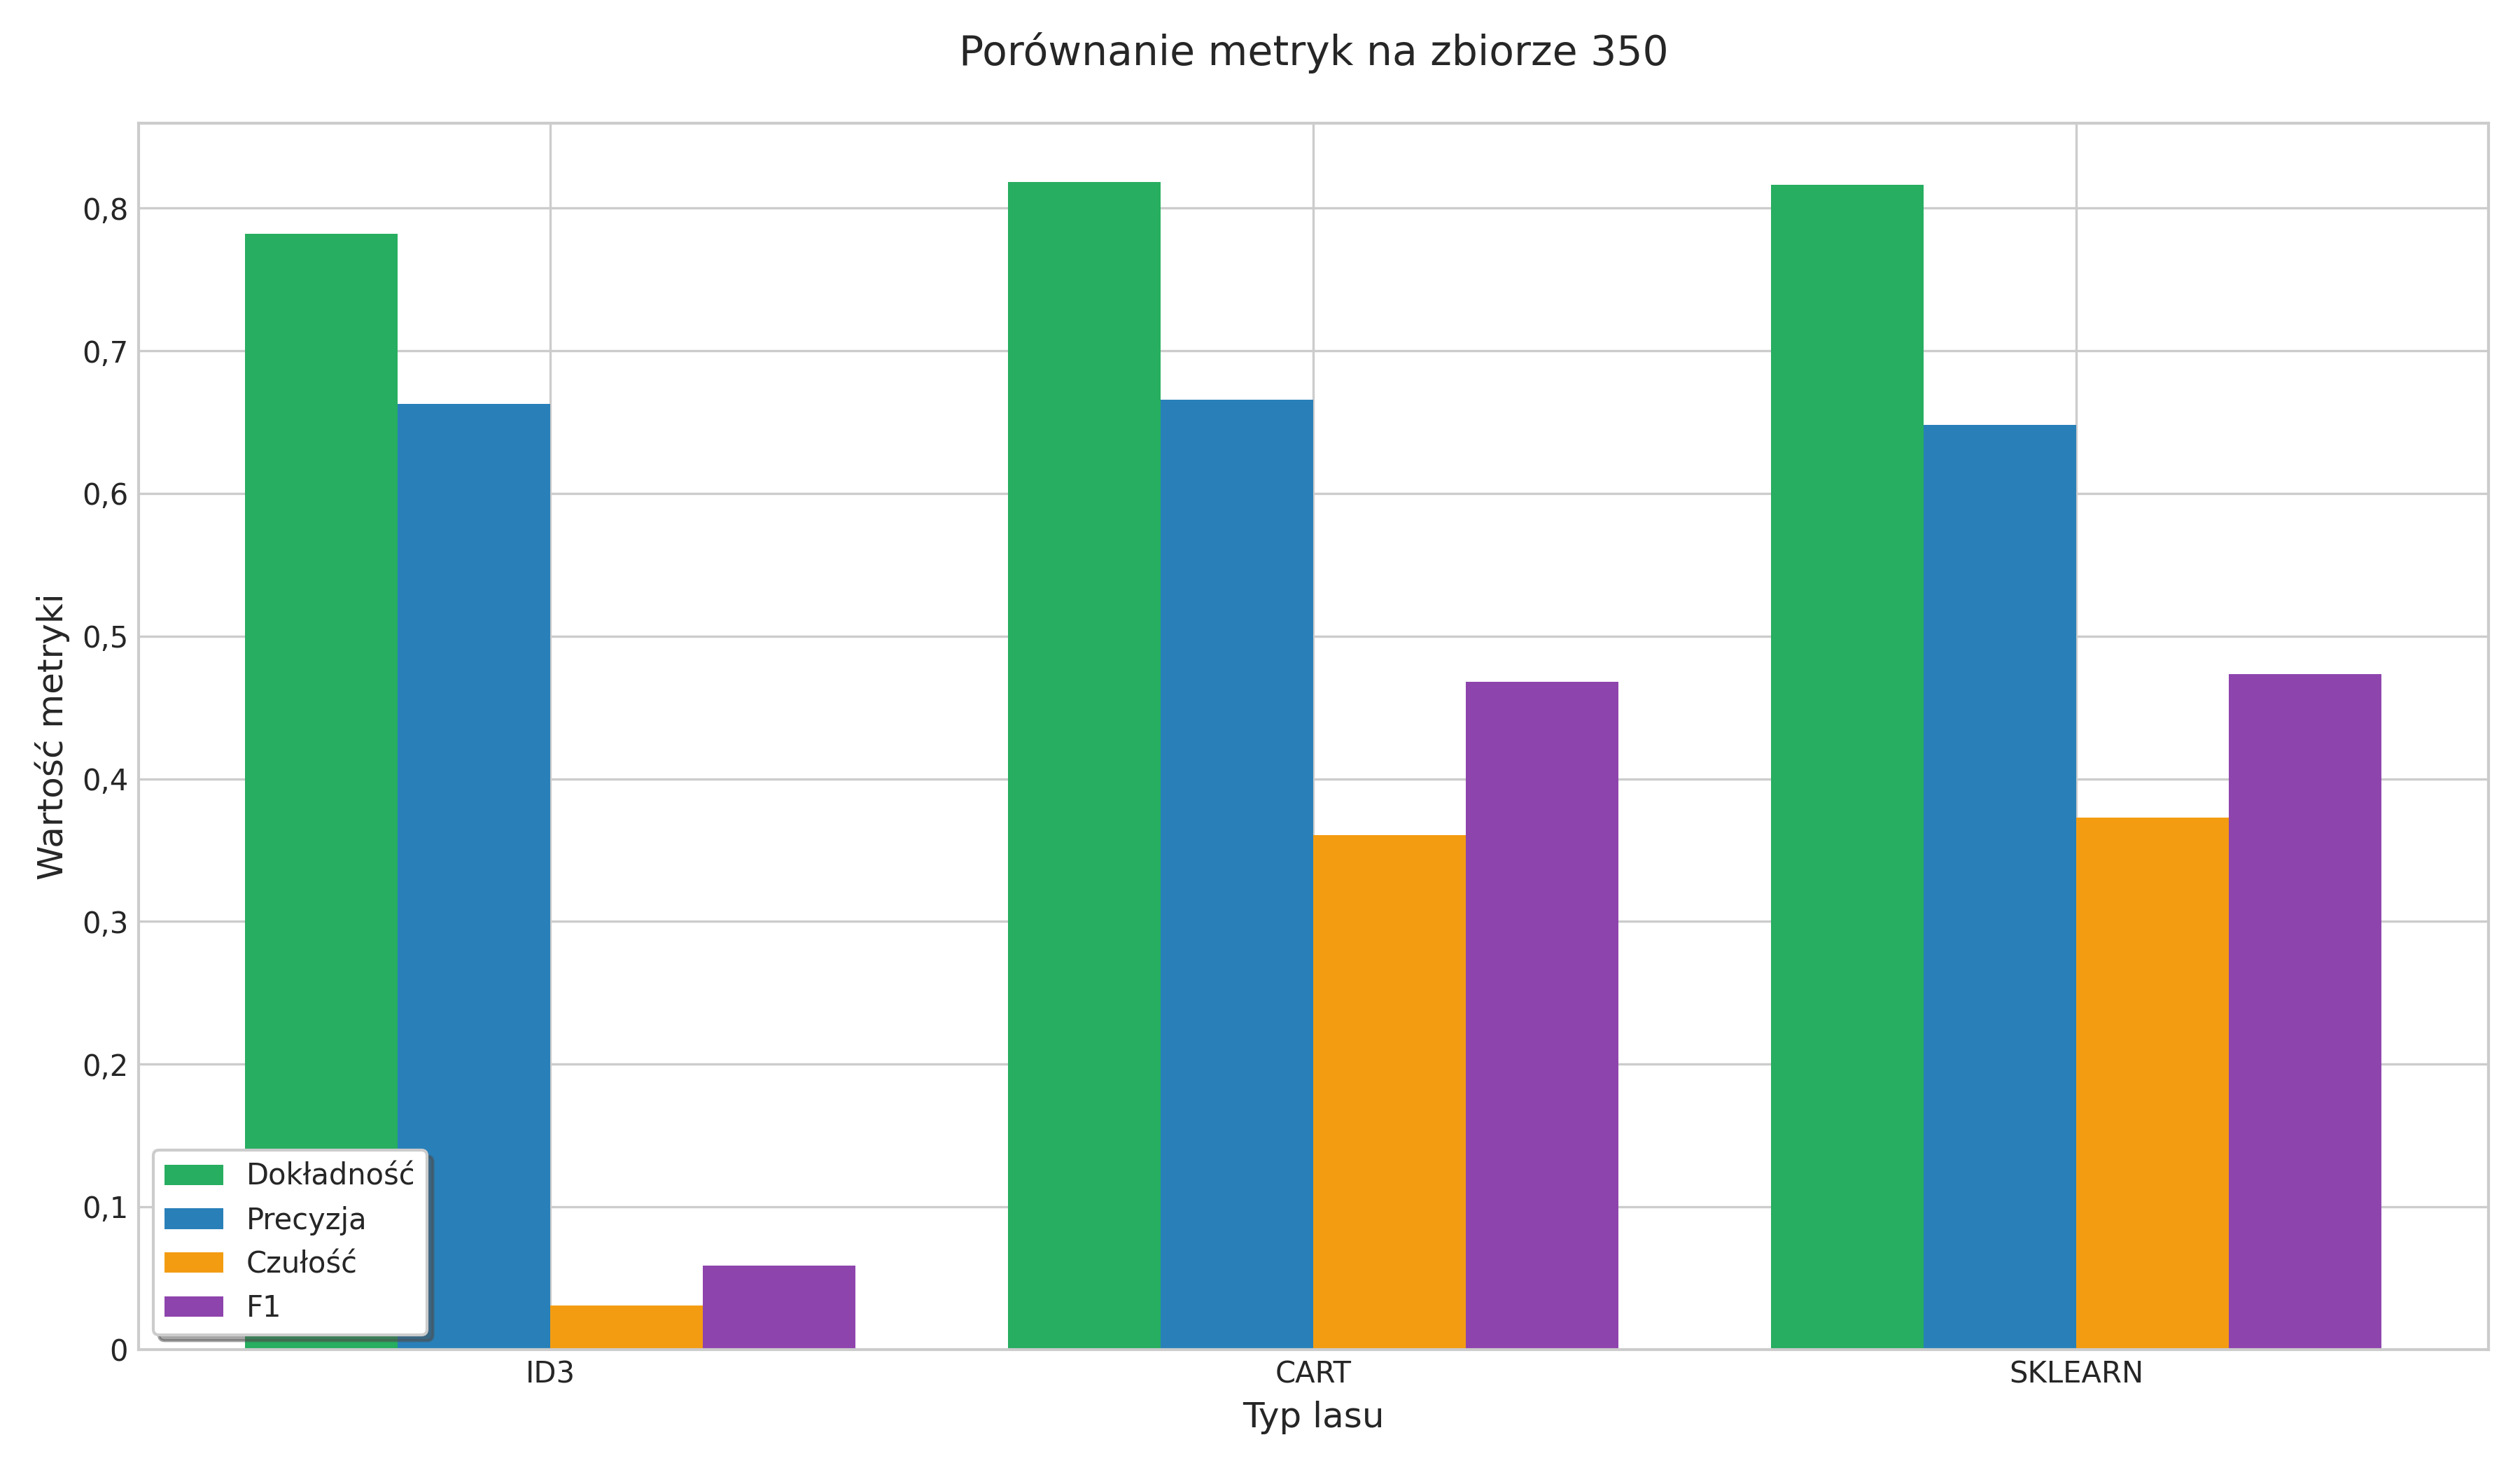
\includegraphics[width=0.9\textwidth]{plots/Compare_on_350_compare_metrics.png}
        \caption{Porównanie modeli dla zbioru 350 - Zaległości płatnicze klientów kart kredytowych.}
        \label{fig:compare_on_350}
    \end{figure}

    \begin{table}[htbp]
        \centering
        \small
        \setlength{\tabcolsep}{4pt}
        \renewcommand{\arraystretch}{1.2}

        \begin{minipage}[t]{0.48\textwidth}
            \centering
            \caption{\textbf{Dokładność} - Typ lasu (zbiór 350)}
            \label{tab:Compare_on_350_acc}
            \begin{tabular}{r|r|r|r|r}
                \toprule
                Typ lasu & Średnia & Std & Maks & Min \\
                \hline
                \textbf{CART} & \textbf{0,818} & \textbf{0,002} & \textbf{0,822} & \textbf{0,816} \\
                SKLEARN & 0,816 & 0,002 & 0,821 & 0,812 \\
                \bottomrule
            \end{tabular}
        \end{minipage}
        \hfill
        \begin{minipage}[t]{0.48\textwidth}
            \centering
            \caption{\textbf{Precyzja} - Typ lasu (zbiór 350)}
            \label{tab:Compare_on_350_prec}
            \begin{tabular}{r|r|r|r|r}
                \toprule
                Typ lasu & Średnia & Std & Maks & Min \\
                \hline
                \textbf{CART} & \textbf{0,666} & \textbf{0,008} & \textbf{0,680} & \textbf{0,650} \\
                SKLEARN & 0,648 & 0,012 & 0,671 & 0,623 \\
                \bottomrule
            \end{tabular}
        \end{minipage}

        \vspace{0.5cm}

        \begin{minipage}[t]{0.48\textwidth}
            \centering
            \caption{\textbf{Czułość} - Typ lasu (zbiór 350)}
            \label{tab:Compare_on_350_rec}
            \begin{tabular}{r|r|r|r|r}
                \toprule
                Typ lasu & Średnia & Std & Maks & Min \\
                \hline
                CART & 0,361 & 0,008 & 0,377 & 0,346 \\
                \textbf{SKLEARN} & \textbf{0,373} & \textbf{0,008} & \textbf{0,388} & \textbf{0,353} \\
                \bottomrule
            \end{tabular}
        \end{minipage}
        \hfill
        \begin{minipage}[t]{0.48\textwidth}
            \centering
            \caption{\textbf{F1} - Typ lasu (zbiór 350)}
            \label{tab:Compare_on_350_f1}
            \begin{tabular}{r|r|r|r|r}
                \toprule
                Typ lasu & Średnia & Std & Maks & Min \\
                \hline
                CART & 0,468 & 0,007 & 0,483 & 0,456 \\
                \textbf{SKLEARN} & \textbf{0,473} & \textbf{0,007} & \textbf{0,487} & \textbf{0,459} \\
                \bottomrule
            \end{tabular}
        \end{minipage}
    \end{table}

    Wariant bazowy oraz zmodyfikowany uzyskały bardzo zbliżone do siebie wyniki.
    Nie da się jednoznacznie wskazać lepszego modelu na tym zbiorze danych.

\section{Wnioski}

Przeprowadzona analiza nie wykazała jednoznacznie, czy modyfikacje lasu losowego w postaci wyboru atrybutów podziału na podstawie turnieju
przekładają się na poprawę jakości modelu. W przypadku niektórych zbiorów danych mogą one pozwalać na uzyskanie lepszych wyników przez zwiększenie
różnorodności drzew w lesie, ale również dla danych o innej charakterystyce mogą nie prowadzić do żadnej poprawy, a nawet powodować pogorszenie
zachowania modelu. Potencjalne zastosowanie tej modyfikacji w praktyce wymagałoby przeprowadzenia analizy na specyficznym zbiorze danych
przypisanym do danego problemu, aby ocenić jej skuteczność w konkretnym przypadku.
W praktyce nasza implementacja drzewa CART różni się od standardowej implementacji z biblioteki scikit-learn sposobem w jaki różnicowany jest zbiór atrybutów biorących udział w tworzeniu podziału węzła.
W naszej implementacji wybór atrybutów realizowany jest poprzez turniej (na wzór turnieju w algorytmach ewolucyjnych) - możliwe są powtórzenia atrybutów. Sprowadza się to do losowania ze zwracaniem,
podczas gdy w bibliotece scikit-learn wybór ten jest realizowany poprzez losowanie bez zwracania tylu atrybutów, ile wskazuje parametr \texttt{max\_features}.


\end{document}

